\documentclass[twoside,11pt]{article}

% Any additional packages needed should be included after jmlr2e.
% Note that jmlr2e.sty includes epsfig, amssymb, natbib and graphicx,
% and defines many common macros, such as 'proof' and 'example'.
%
% It also sets the bibliographystyle to plainnat; for more information on
% natbib citation styles, see the natbib documentation, a copy of which
% is archived at http://www.jmlr.org/format/natbib.pdf

% Use of packages.
\usepackage{jmlr2e}
\usepackage[table]{xcolor}
\usepackage{times}
\usepackage[colorinlistoftodos]{todonotes}
\usepackage{amsmath,amsfonts,amssymb}
\usepackage{pict2e}
\usepackage{graphicx}
\usepackage{subfigure}
\usepackage{bm}
\usepackage{url}
% \usepackage{amssymbmb}
\usepackage{soul,color}
\usepackage{graphicx,float,wrapfig}
\usepackage{xr}
\usepackage[english]{babel}
\usepackage{multirow}
\usepackage{slashbox}
\usepackage{tabularx}
\usepackage{placeins}


\usepackage{natbib}
\usepackage{algorithm}
\usepackage{algorithmic}
\usepackage{hyperref}
\usepackage{relsize}
\usepackage{natbib}
\usepackage{soul,color}

% Commands.
\newcommand{\dataset}{{\cal D}}
\newcommand{\fracpartial}[2]{\frac{\partial #1}{\partial  #2}}
\newcommand{\xv}{\bm{x}}
\newcommand{\Xv}{\bm{X}}

\newcommand{\yv}{\bm{y}}
\newcommand{\Yv}{\bm{Y}}
\newcommand{\yvhat}{\hat{\yv}}
\newcommand{\yhat}{\hat{y}}

\newcommand{\zv}{\bm{z}}
\newcommand{\Zv}{\bm{Z}}

\newcommand{\sv}{\bm{s}}
\newcommand{\Sv}{\bm{S}}

\newcommand{\hv}{\bm{h}}
\newcommand{\Hv}{\bm{H}}

\newcommand{\gv}{\bm{g}}
\newcommand{\Gv}{\bm{G}}

\newcommand{\av}{\bm{a}}
\newcommand{\Av}{\bm{A}}
\newcommand{\algo}{\mathcal{A}}

\newcommand{\Bv}{\bm{B}}

\newcommand{\regret}{\mathcal{R}}

\newcommand{\vv}{\bm{v}}
\newcommand{\Vv}{\bm{V}}

\newcommand{\wv}{\bm{w}}
\newcommand{\Wv}{\bm{W}}
\newcommand{\fv}{\bm{f}}
\newcommand{\ev}{\bm{e}}

\newcommand{\uv}{\bm{u}}
\newcommand{\Uv}{\bm{U}}
\newcommand{\loss}{\ell}

\newcommand{\defEq}{\equiv}
\newcommand{\eat}[1]{}

\newcommand{\ud}{\mathrm{d}}
\newcommand{\diag}{\mathrm{diag}}
\newcommand{\risk}{\mathcal{R}}
\newcommand{\prob}{\mathcal{P}}
\newcommand{\sign}{\mathrm{sign}}
\newcommand{\etav}{\bm \eta}
\newcommand{\thetav}{\bm{\theta}}
\newcommand{\Thetav}{\bm{\Theta}}
\newcommand{\phiv}{\bm{\phi}}
\newcommand{\Phiv}{\bm{\Phi}}
\newcommand{\muv}{\bm \mu}
\newcommand{\nuv}{\bm \nu}
\newcommand{\psiv}{\bm \psi}
\newcommand{\xiv}{\bm \xi}
\newcommand{\alphav}{\bm \alpha}
\newcommand{\betav}{\bm \beta}
\newcommand{\lambdav}{\bm \lambda}
\newcommand{\piv}{\bm \pi}
\newcommand{\barpiv}{\bm{\bar{\pi}}}
\newcommand{\omegav}{\bm \omega}
\newcommand{\gammav}{\bm \gamma}
\newcommand{\Sigmav}{\bm \Sigma}
\newcommand{\Mv}{\bm{\mathcal{M}}}
\newcommand{\ep}{\mathbb{E}}
\newcommand{\KL}{\textbf{KL}}
\newcommand{\B}{\mathrm{Beta}}
\newcommand{\M}{\mathrm{Mult}}
\newcommand{\Ber}{\mathrm{Bernoulli}}
\newcommand{\uniform}{\mathrm{U}}
\newcommand{\N}{\mathcal{N}}
\newcommand{\var}{\mathbb{V}}
\newcommand{\real}{\mathbb{R}}
\newcommand{\E}{\mathbb{E}}
\newcommand{\model}{\mathcal{M}}
\newcommand{\ms}{\mathbb{M}}
\newcommand{\data}{\mathcal{D}}
\newcommand{\Dir}{\text{Dir}}
\newcommand{\barzv}{\bm{\bar{z}}}
\newcommand{\subto}{\text{s.t.:}}
\newcommand{\normal}{\mathcal{N}}
\newcommand{\ind}{\mathbb{I}}
\newcommand\paMedLDAave{$\text{paMedLDA}^{\text{ave}}$~}
\newcommand\paMedLDAgibbs{$\text{paMedLDA}^{\text{gibbs}}$~}
\newcommand\paMedLDAmtave{$\text{paMedLDAmt}^{\text{ave}}$~}
\newcommand\paMedLDAmtgibbs{$\text{paMedLDAmt}^{\text{gibbs}}$~}
\newcommand\paMedHDPave{$\text{paMedHDP}^{\text{ave}}$~}
\newcommand\paMedHDPgibbs{$\text{paMedHDP}^{\text{gibbs}}$~}
\newcommand\MedHDPave{$\text{MedHDP}^{\text{ave}}$~}
\newcommand\MedHDPgibbs{$\text{MedHDP}^{\text{gibbs}}$~}
\newcommand\MedHDPmtave{$\text{MedHDPmt}^{\text{ave}}$~}
\newcommand\MedHDPmtgibbs{$\text{MedHDPmt}^{\text{gibbs}}$~}
\newcommand\MedLDAgibbs{$\text{MedLDA}^{\text{gibbs}}$~}
\def\indicator{{\mathbb I}}

\newcommand{\theHalgorithm}{\arabic{algorithm}}
\newcommand{\fix}{\marginpar{FIX}}
\newcommand{\new}{\marginpar{NEW}}
\newcommand\refeq[1]{(\ref{#1})}




\newcommand{\strin}[1]{\todo[size=\small, color=green!40]{\bf\sf  #1}}


%\newtheorem{theorem}{Theorem}[section]
%\newtheorem{lemma}[theorem]{Lemma}
%\newtheorem{observation}[theorem]{Observation}
%\newtheorem{definition}[theorem]{Definition}
%\newtheorem{proposition}[theorem]{Proposition}
%\newtheorem{corollary}[theorem]{Corollary}

\newcommand{\argmax}{arg\,max}
\newcommand{\argmin}{arg\,min}

\setlength{\marginparwidth}{1.2in}
\usepackage{color}
\newcommand{\junx}[1]{{\color{red}{\bf\sf #1}}}
\newcommand{\jun}[1]{\marginpar{\color{blue}\tiny{Jun: #1}}}

% Heading arguments are {volume}{year}{pages}{submitted}{published}{author-full-names}
\jmlrheading{1}{2014}{1-48}{4/00}{10/00}{Tianlin Shi and Jun Zhu}

% Short headings should be running head and authors last names

\ShortHeadings{Online Bayesian Passive-Aggressive Learning}{Shi and Zhu}
\firstpageno{1}

\begin{document}

\title{Online Bayesian Passive-Aggressive Learning\thanks{Correspondence should be addressed to J. Zhu.}}

\author{\name Tianlin Shi \email tianlins@cs.stanford.edu \\
       \addr Stanford Artificial Intelligence Laboratory (SAIL)\\
       Stanford University \\
       Stanford, CA. 94305.
       \AND
       \name Jun Zhu \email dcszj@mail.tsinghua.edu.cn \\
       \addr State Key Lab of Intelligent Technology and Systems \\
       \addr Tsinghua National Lab for Information Science and Technology \\
       \addr Department of Computer Science and Technology\\
       Tsinghua University \\
       Beijing, 100084 China}

\editor{}

\maketitle

\begin{abstract}%
%Online Passive-Aggressive (PA) learning is an effective framework for performing max-margin online learning. But the deterministic formulation and estimated single large-margin model could limit its capability in discovering descriptive structures underlying complex data. In contrast, regularized Bayesian inference methods with max-margin posterior regularization admit the great flexibility of revealing latent structures, but existing batch inference algorithms are not applicable to streaming data.
We present online Bayesian Passive-Aggressive (BayesPA) learning, a generic online learning framework for hierarchical Bayesian models with max-margin posterior regularization. We provide provable Bayesian regret bounds for both averaging classifiers and Gibbs classifiers. We show that BayesPA subsumes the standard online Passive-Aggressive (PA) learning and more importantly extends naturally to incorporate latent variables for both parametric and nonparametric Bayesian inference, therefore providing great flexibility for explorative analysis. As an important example, we apply BayesPA to topic modeling and derive efficient online learning algorithms for max-margin topic models. We further develop nonparametric BayesPA topic models to resolve the unknown number of topics. Experimental results on 20newsgroups and a large Wikipedia multi-label data set (with 1.1 millions of training documents and 0.9 million of unique terms in the vocabulary) show that our approaches significantly improve time efficiency while maintaining comparable results with the batch counterpart methods.

%Existing inference paradigms for max-margin Bayesian learning require multi-passes through the dataset. In this paper, we present Bayesian Passive-Aggressive (PA) learning for supervised Bayesian models in the presence of online streaming data. Conceptually, our approach generalizes the online Passive-Aggressive algorithms by \citep{shalev2003online}, with new techniques to deal with latent variables. As case studies, we apply Bayesian PA learning to two maximum entropy discriminant models. Empirical experiments on real datasets show that our approach yield results comparable to batch counterparts in one pass, and significantly outperforms other online learning algorithms.
\end{abstract}

% Manual newpage inserted to improve layout of sample file - not
% needed in general before appendices/bibliography.

\section{Introduction}

% abstract knowledge -> models with structure -> Bayesian nonparametrics -> max-margin e.g. topic model.
% online learning.
% we propose bpal. -> generalize pa ->
% bpal applied to topic modeling.

In the Big Data era, it is becoming a norm that massive data corpora need to be efficiently handled in many application areas, while standard batch learning algorithms may fail. This has lead to the fast growing interests in developing scalable online or distributed learning algorithms. This paper focuses on online learing, a process of answering a sequence of questions (e.g., which category does a document belong to?) given knowledge of the correct answers (e.g., the true category labels) to previous questions. Such a process is especially suitable for the applications with streaming data. For the applications with a fixed large-scale data set, online learning algorithms can effectively explore data redundancy relative to the model to be learned, by repeatedly subsampling the data; and they often lead to faster convergence to satisfactory results than the batch counterpart algorithms. Among the many popular algorithms, online Passive-Aggressive (PA) learning~\citep{crammer2006pa} provides a generic framework of performing online learning for large-margin methods (e.g., SVMs), with many applications in natural language processing and text mining~\citep{McDonald2005parsing, chiang2008emnlp}. Though enjoying strong discriminative ability that is preferable for predictive tasks, existing online PA methods are formulated as a point estimate problem by optimizing some deterministic objective function. This may lead to some inconvenience. For example, a single large-margin model is often less than sufficient in describing complex data, such as those with rich underlying structures. %Moreover, the non-Bayesian formulation could restrict its marriage with Bayesian statistics for developing new methods.

On the other hand, Bayesian methods enjoy the great flexibility in describing the possible underlying structures of complex data by incorporating a hierarchy of latent variables. Moreover, the recent progress on nonparametric Bayesian methods~\citep{hjort2010bayesian,teh2006hierarchical} further provides an increasingly important framework that allows the Bayesian models to have an unbounded model complexity, e.g., an infinite number of components in a mixture model~\citep{hjort2010bayesian} or an infinite number of units in a latent feature model~\citep{Griffiths:tr05}, and to adapt when the learning environment changes. In particular, adaptation to the changing environment is of great importance in online learning. For Bayesian models, one challenging problem is posterior inference, for which both variational and Monte Carlo methods can be too expensive to be applied to large-scale applications. To scale up Bayesian inference, much progress has been made on developing stochastic variational Bayes~\citep{hoffman2013stochastic,mimno2012sparse} and stochastic gradient Monte Carlo~\citep{welling2011bayesian,welling2012mc} methods, which repeatedly draw samples from a given finite data set. To deal with the potentially unbounded streaming data, streaming variational Bayes methods~\citep{broderick2013streaming} have been developed as a general framework, with an application to topic models for learning latent topic representations. However, due to the generative nature, Bayesian models are lack of the discriminative ability of large-margin methods and are usually less than sufficient in performing discriminative tasks.

Successful attempts have been made to bring large-margin learning and Bayesian methods together to solve supervised learning tasks using flexible Bayesian latent variable models. For example, maximum entropy discrimination (MED) made a significant advance in conjoining max-margin learning and Bayesian generative models, in the context of univariate prediction~\citep{jaakkola1999maximum} and structured output prediction~\citep{Zhu:jmlr09}. Recently, much attention has been devoted to generalizing MED to incorporate latent variables and perform nonparametric Bayesian inference in various contexts, including topic modeling~\citep{zhu2012medlda}, matrix factorization~\citep{xu2013fast}, and multi-task learning~\citep{jebara2011mtl,zhu2013bayesian}. Regularized Bayesian inference (RegBayes)~\citep{zhu2013bayesian} provides a unified framework for Bayesian models to perform max-margin learning, where the max-margin principle is incorporated through imposing posterior constraints to an information-theoretical optimization problem. By solving this problem involving latent variables, RegBayes can uncover structures that support the supervised learning tasks. RegBayes subsumes the standard Bayes' rule and is more flexible in incorporating domain knowledge or max-margin constraints. Though flexible in discovering latent structures and powerful in discriminative predictions, posterior inference in such models remains a challenge. By exploring data augmentation techniques, recent progress has been made to develop efficient MCMC methods~\citep{zhugibbs2013}, which can also be implemented in distributed clusters~\citep{zhu2013scalable}. However, these batch-learning methods are not applicable to streaming data, and they do not explore the statistical redundancy in large-scale corpura either. %Therefore, it is desirable to develop efficient online algorithms for these Bayesian max-margin models.

To address the above problems of both online PA on incorporating flexible latent structures and Bayesian max-margin models on scalable streaming inference, this paper presents online Bayesian Passive-Aggressive (BayesPA) learning, a general framework of performing online learning for Bayesian max-margin models. %, with the great flexibility of Bayesian methods for explorative analysis as well as the strong discriminative ability of large-margin methods for predictive tasks.
We show that online BayesPA subsumes the standard online PA when the underlying model is linear and the parameter prior is Gaussian (See Table~\ref{table:relationship} for its close relationships with streaming variational Bayes and RegBayes). We characterize the performance of BayesPA by providing regret bounds for both the case when using an averaging classifier and the case when using a Gibbs classifier. We further show that one major significance of BayesPA is its natural generalization to incorporate a hierarchy of latent variables for both parametric and nonparametric Bayesian inference, therefore allowing online BayesPA to have the great flexibility of (nonparametric) Bayesian methods for explorative analysis as well as the strong discriminative ability of large-margin learning for predictive tasks. As concrete examples, we apply the theory of online BayesPA to topic modeling and derive efficient online learning algorithms for max-margin supervised topic models~\citep{zhu2012medlda}. We further develop efficient online learning algorithms for the nonparametric max-margin topic models, an extension of the nonparametric topic models~\citep{teh2006hierarchical} for predictive tasks. Extensive empirical results on real data sets demonstrate significant improvements on time efficiency and maintenance of comparable results with the batch counterparts.

The paper is structured as follows. We discuss the related work in Section~\ref{sec:relatedwork}, and review the preliminary knowledge in Section~\ref{sec:pre}. Then, we move on to the detailed description of BayesPA in Section~\ref{sec:bpal}, and present the theoretical analysis in Section~\ref{sec:theory}. Section~\ref{sec:pamedlda} presents the concrete instantiations on topic modeling, and Section~\ref{sec:extensions} presents the extensions to nonparametric topic models and multi-task learning. Section~\ref{sec:exp} presents experimental results. Finally, Section~\ref{sec:con} concludes this paper with future directions discussed.

\section{Related Work}\label{sec:relatedwork}

As a well-established learning paradigm, online learning is of both theoretical and practical interest. The goal of online learning is to make a sequence of decisions, such as classifications and regression, and use the knowledge extracted from previous correct answers to produce decisions on incoming ones. The root of online learning could be traced back to early studies of repeated games~\citep{hannan1957approximation}, where an agent dynamically makes choices with the summary of past information. The idea became popular with the advent of Perceptron algorithms~\citep{rosenblatt1958perceptron}, which adopt an additive update rule for the classifier weights, and its multiplicative counterpart is the Winnow algorithm~\citep{littlestone1988learning}. The class of online multiplicative algorithms was further generalized by Adaboost~\citep{freund1997decision} in a decision theoretic sense and now widely applied to various fields of study~\citep{arora2012multiplicative}.

As a member of the family of weight updating methods, online Passive-Aggressive (PA) algorithms provide a generic online learning framework for max-margin models, first presented by~\citet{crammer2006pa}. In particular, they considered loss functions that enforce max-margin constraints, and showed that surprisingly simple update rules could be derived in closed forms. Motivated by online PA learning and to handle unbalanced training sets, \cite{dredze2008confidence} proposed confidence-weighted learning, which maintains a Gaussian distribution of the classifier weights at each round and replaces the max-margin constraint in PA with a probabilistic constraint enforcing confidence of classification. Within the same framework, \cite{pereira2008exact} derived a new convex form of the constraint and demonstrated performance improvements through empirical evaluations.

The theoretical analysis of online learning typically relies on the notion of \emph{regret}, which is the average loss incurred by an adaptive online learner on streaming data versus the best achievable through a single fixed model having the hindsight of all data~\citep{murphy2012machine_reget}. It can be shown that the notion of \emph{regret} is closely related to \emph{weak duality} in convex optimization, which brings online learning to the algorithmic framework of convex repeated games~\citep{shalev2006convex}.

Although the classical regime of online learning is based on decision theory, recently much attention has been paid to the theory and practice of online probabilistic inference in the context of Big Data. Rooted either in variational inference or Monte Carlo sampling methods, there are broadly two lines of work on the topic of online Bayesian inference. Stochastic variational inference (SVI)~\citep{hoffman2013stochastic} is a stochastic approximation algorithm for mean-field variational inference. By approximating the nature gradients in maximizing the evidence lower bound with stochastic gradients sampled from data points, \cite{hoffman2013stochastic} demonstrated scalable inference of topic models on large corpora. \cite{mimno2012sparse} showed the performance of SVI could be improved through structured mean-field assumptions and locally collapsed variational inference. SVI is also applicable to the stochastic inference of nonparametric Bayesian models, such as hierarchical Dirichlet process~\citep{wang2011onlinealgo, wang2012truncation}.

There is also a large body of work on extending Monte Carlo methods to the online setting. A classic approach is sequential Monte Carlo methods (SMC) or particle filters~\citep{doucet2009tutorial}, which arose from the numerical estimation of state-space models. For example,  through Rao-Blackwellized particle filters~\citep{doucet2000rao}, one could obtain online inference algorithms for latent Dirichlet allocation~\citep{canini2009online}. To tackle the sparsity issues and inadequate coverage of particles, \cite{steinhardt2014filtering} leveraged ``abstract particles'' to represent entire regions of the sample space. Recently, \cite{korattikara2014austerity} introduced an approximate Metropolis-Hasting rule based on sequential hypothesis testing that allows accepting and rejecting samples using only a fraction of the data. As an alternative,~\cite{bardenet2014towards} proposed an adaptive sampling strategy of Metropolis-Hastings from a controlled perturbation of the target distribution. With elegant use of gradient information that Metropolis-Hastings algorithms neglected, a line of work~\citep{welling2011bayesian, welling2012mc, patterson2013stochastic} also developed stochastic gradient methods based on Langevin dynamics.

While most online Bayesian inference methods have adopted a \emph{stochastic approximation} of the posterior distribution by sub-sampling a given finite data set, in many applications data arrives in stream so that the data set is changing over time and its size is unknown. To relax the previous request on knowing the data size, \cite{broderick2013streaming} made streaming updates to the estimated posterior and demonstrated the advantage of streaming variational Bayes (SVB) over stochastic variational inference. As will be discussed in this paper, BayesPA also does not impose assumptions on the size of data set and works on streaming data.

%\strin{svm is generative?}
The idea to discriminatively train univariate or structured output classifiers was popularized by the seminal work on support vector machines~\citep{Vapnik:95} and max-margin Markov networks (aka structural SVMs)~\citep{koller2003max}. In the sequel, research on developing max-margin models with latent variables has received increasing attention, because of the promise to capture underlying complex structures of the problems. A promising line of work focused on Bayesian approaches, and one representative is maximum entropy discrimination (MED)~\citep{jaakkola1999maximum,jebara2001discriminative,Zhu:jmlr09}, which learns distributions of model parameters discriminatively from labeled data. MedLDA~\citep{zhu2012medlda} extended MED to infer latent topical structure from data with large margin constraints on the target posteriors. Similarly, nonparametric Bayesian max-margin models have also been developed, such as infinite SVMs (iSVM)~\citep{zhu2011infinite} for building SVM classifiers with latent mixture structure, and infinite latent SVMs (iLSVM)~\citep{zhu2013bayesian} for automatic discovering predictive features for SVMs. Furthermore, the idea of nonparametric Bayesian learning has been widely applied to link prediction~\citep{zhu2012maxlink}, matrix factorization~\citep{xu2013fast}, etc. Regularized Bayesian inference (RegBayes)~\citep{zhu2013bayesian} provides a unified framework for performing max-margin learning of (nonparametric) Bayesian models, where the max-margin principle was incorporated through imposing posterior constraints to a variational formulation of the standard Bayes' rule.

Max-margin Bayesian learning in the batch mode has already been one of the common challenges facing this class of models. Despite its general intractability, efficient algorithms have been proposed under different settings. One way is to solve the problem via variational inference under a mean-field~\citep{zhu2012medlda} or structured mean-field~\citep{jiang2012monte} assumption. Recently, \cite{zhugibbs2013} provided a key insight in deriving efficient Monte Carlo methods without making strict assumptions. Their technique is based on a data augmentation formulation of the expected margin loss. Based on similar techniques, fast inference algorithms have also been developed for generalized relational topic models~\citep{chen2013generalized}, matrix factorization~\citep{xu2013fast}, etc. Data augmentation (DA) refers to the method of introducing augmented variables along with the observed data to make their joint distribution tractable. The technique was popularized in the statistics community by the well-known expectation-maximization algorithm (EM) ~\citep{dempster1977maximum} for maximum likelihood estimation with missing data. For posterior inference, the technique is popularized by~\cite{tanner1987calculation} in statistics and by \cite{swendsen1987nonuniversal} for the Ising and Potts models in physics. For a broader introduction to DA methods, we refer the readers to~\cite{van2001art}.

Finally, our conference version of the paper~\citep{shi2014bayespa} has introduced some preliminary work, which we largely extend.


\section{Preliminaries}\label{sec:pre}
% \junx{Online BayesPA is a streaming version of RegBayes; is a max-margin extension of streaming variational Bayes; and is a Bayesian version of online PA. Let's put the basics of the three topics here; and make the connection explicit in later sections.}

This section reviews the preliminary knowledge that is needed to develop online Bayesian Passive-Aggressive learning. The relationships with BayesPA will be summarized in Table~\ref{table:relationship} later.

\subsection{Online Passive-Aggressive Learning}\label{sec:pa}

Based on a decision-theoretic view, the goal of online supervised learning is to minimize the cumulative loss for a certain prediction task from the sequentially arriving training samples. Online Passive-Aggressive (PA) learning \citep{crammer2006pa} achieves this goal by updating some parametric model $\bm{w} \in \real^K$ (e.g., the weights of a linear SVM) in an online manner with the instantaneous losses from arriving data $\{\bm{x}_t\}_{t \geq 0}$ ($\xv_t \in \real^K$) and corresponding responses $\{y_t\}_{t \geq 0}$. The losses $\ell_\epsilon(\bm{w}; \bm{x}_t, y_t)$, as they consider, could be the hinge loss $(\epsilon-y_t \wv^\top \xv_t)_+$ for binary classification ($y_t \in \{0,1\}$) or the $\epsilon$-insensitive loss $(|y_t- \wv^\top \xv_t|-\epsilon)_+$ for regression ($y_t \in \mathbb{R}$), where $\epsilon$ is a hyper-parameter and $(x)_+ = \max(0,x)$. The online Passive-Aggressive update rule is then derived by defining the new weight $\bm{w}_{t+1}$ as the solution to the following optimization problem:
\begin{equation}\label{eq:pa}
\min_{\bm{w}}{\frac{1}{2} ||\bm{w}-\bm{w_{t}}||^2} ~~~ \text{s.t.:} ~ \ell_{\epsilon}(\bm{w}; \bm{x}_t, y_t) = 0,
\end{equation}
where $\Vert \cdot \Vert^2$ is the Euclidean 2-norm. Intuitively, if $\bm{w_t}$ suffers no loss from the new data, i.e., $\ell_{\epsilon}(\bm{w}_t; \bm{x}_t, y_t) = 0$, the algorithm \emph{passively} assigns $\bm{w}_{t+1} = \bm{w}_t$; otherwise, it aggressively projects $\bm{w_t}$ to the feasible zone of parameter vectors that attain zero loss on the new data. With provable regret bounds, \cite{crammer2006pa} showed that online PA algorithms could achieve comparable results to the optimal classifier $\bm{w}^*$, which has the hindsight of all data. In practice, in order to account for inseparable training samples, soft margin constraints are often adopted and the resulting PA learning problem is
\begin{equation}\label{eq:pa-soft}
\min_{\bm{w}}{\frac{1}{2} ||\bm{w}-\bm{w_{t}}||^2} + 2 c \cdot \ell_{\epsilon}(\bm{w}; \bm{x}_t, y_t),
\end{equation}
where $c$ is a positive regularization parameter and the constant factor $2$ is included for simplicity as will be clear soon. For problems~(\ref{eq:pa}) and (\ref{eq:pa-soft}) with samples arriving one at a time, closed-form solutions can be derived~\citep{crammer2006pa}. For example, for the binary hinge loss the update rule is $\wv_{t+1} = \wv_t + \tau_t y_t \xv_t$, where $\tau_t = \min(2c, \max(0,\epsilon-y_t \wv^\top \xv_t)/||\xv_t||^2)$; and for the $\epsilon$-insensitive loss, the update rule is $\wv_{t+1} = \wv_t+\text{sign}(y_t-\wv^\top \xv_t) \tau_t \xv_t$, where $\tau_t = \max(0,\epsilon-y_t \wv^\top \xv_t)/||\xv_t||^2$.


\subsection{Streaming Variational Bayes}

For Bayesian models, Bayes' rule naturally leads to a streaming update procedure for online learning. Specifically, suppose the data $\{\xv_t\}_{t \geq 0}$ are generated i.i.d. according to a distribution $p(\xv | \wv)$ and the prior $p(\wv)$ is given. Bayes' theorem implies that the posterior distribution of $\wv$ given the first $T$ samples ($T \geq 1$) satisfies
\begin{equation}\label{eq:stream-Bayes-update}
p(\wv | \{\xv_t\}_{t=0}^T) \propto p(\wv | \{\xv_t\}_{t=0}^{T-1}) p(\xv_T | \wv).
\end{equation}
In other words, the posterior after observing the first $T-1$ samples is treated as the prior for the incoming data point.

This natural streaming Bayes' rule, however, is often intractable to compute, especially for complex models (e.g., when latent variables are present). Streaming variational Bayes (SVB)~\citep{broderick2013streaming} suggests that a variational approximation should be adopted and it practically works well. Specifically, let $\algo$ be any algorithm that calculates an approximate posterior $q(\wv) = \algo(\Xv, q_0(\wv))$ based on data $\Xv$ and prior $q_0(\wv)$. Then, the recursive formula for approximate streaming update is:
\begin{equation*}
q(\wv | \{\xv_t\}_{t=0}^T) = \algo\left( \xv_T, q(\wv | \{\xv_t\}_{t=0}^{T-1}) \right).
\end{equation*}
The choice of $\algo$ can be problem-specific. For topic modeling, \cite{broderick2013streaming} showed that one may adopt mean-field variational Bayes~\citep{wainwright2008graphical}, expectation propagation~\citep{minka2001expectation}, and one-pass posterior approximation algorithms using stochastic variational inference~\citep{hoffman2013stochastic} or sufficient statistics update~\citep{honkela2003line, luts2013real}. By applying the streaming update in a distributed setting asynchronously, SVB could also be scaled up across multiple computer clusters~\citep{broderick2013streaming}.



\subsection{Regularized Bayesian Inference}

The decision-theoretic and Bayesian view of learning can be reciprocal. For example, it would be beneficial to combine the flexibility of Bayesian models with the discriminative power of large-margin methods. The idea of regularized Bayesian inference (RegBayes)~\citep{zhu2013bayesian} is to treat Bayesian inference as an optimization problem with an imposed loss function. Mathematically, RegBayes for supervised learning can be formulated as
\begin{equation}\label{eq:regBayes}
\min\limits_{q \in \mathcal{P}}~~ \KL\Big[q(\wv)||p_0(\wv)\Big] - \ep_{q(\wv)} \Big[ \log p(\Xv | \wv) \Big] + 2c \cdot \loss\Big(q(\wv); \Xv, \Yv \Big),
\end{equation}
where $\mathcal{P}$ is the probability simplex, $p(\Xv | \wv)$ is the likelihood function and $\KL$ is the Kullback-Leibler divergence.\footnote{We assume that the model space $\Wv$ is a complete separable metric space endowed with its Borel $\sigma$-algebra $\mathcal{B}(\Wv)$. Let $P_0$ and $Q$ be probability measures on $\Wv$. The Kullback-Leibler (KL) divergence of the probability measure $Q$ with respect to the measure $P_0$ is defined as $\KL[ Q \Vert P_0] = \int \frac{\ud Q}{\ud P_0}(\wv) \log \frac{\ud Q}{\ud P_0}(\wv) \ud P_0(\wv),$ where $\frac{\ud Q}{\ud P_0}(\wv)$ is the Radon-Nikodym derivative~\citep{durret2010}. It is required that $Q$ is absolutely continuous with respect to $P_0$ such that this derivative exists. In the sequel, we further assume that $P_0$ is absolutely continuous with respect to some background measure $\mu$. Thus, there exists a density $p_0$ that satisfies $\ud P_0 = p_0 \ud \mu$ and there also exists a density $q$ that satisfies $\ud Q = q \ud \mu$. Then, the KL-divergence can be expressed as $\KL[ q \Vert p_0 ] = \int q(\wv) \log \frac{q(\wv)}{p_0(\wv)} \ud \mu(\wv)$.}
%Specifically, let $\Wv$ denote the space of feasible models. We assume that $\Wv$ is a complete separable metric space endowed with its Borel $\sigma$-algebra $\mathcal{B}(\Wv)$. Let $P_0$ and $Q$ be probability measures on $\Wv$. The Kullback-Leibler (KL) divergence of the probability measure $Q$ with respect to the measure $P_0$ is defined as $$\KL[ Q \Vert P_0] = \int \frac{\ud Q}{\ud P_0}(\wv) \log \frac{\ud Q}{\ud P_0}(\wv) \ud P_0(\wv),$$
%where $\frac{\ud Q}{\ud P_0}(\wv)$ is the Radon-Nikodym derivative~\citep{durret2010}. It is required that $Q$ is absolutely continuous with respect to $P_0$ such that this derivative exists. In the sequel, we further assume that $P_0$ is absolutely continuous with respect to some background measure $\mu$. Thus, there exists a density $p_0$ that satisfies $\ud P_0 = p_0 \ud \mu$ and there also exists a density $q$ that satisfies $\ud Q = q \ud \mu$. Then, the KL-divergence can be expressed as
%$$\KL[ q \Vert p_0 ] = \int q(\wv) \log \frac{q(\wv)}{p_0(\wv)} \ud \mu(\wv).$$
Note that if the loss $\loss(q(\wv); \Xv, \Yv) = 0$, then the optimal solution is $q^*(\wv) \propto p_0(\wv) p(\Xv | \wv)$, which is just the Bayes' rule. However, when $\loss(q(\wv); \Xv, \Yv) \not= 0$, RegBayes biases the inferred posterior towards discriminating the supervising side-information $\Yv$, with the parameter $c$ controlling the extent of regularization. If the posterior regularization term $\ell(\cdot)$ is a convex function of $q(\wv)$ through the linear expectation operator, \cite{zhu2013bayesian} presented a general representation theorem to characterize the solution to problem~(\ref{eq:regBayes}). To distinguish from the posterior obtained via Bayes' rule, the solution to problem~(\ref{eq:regBayes}) is called {\it post-data posterior}~\citep{zhu2013bayesian}. Many instantiations have been developed following the generic framework of RegBayes to demonstrate its superior performance than standard Bayesian models in various settings, such as topic modeling~\citep{jiang2012monte,zhugibbs2013}, matrix factorization~\citep{xu2013fast}, link prediction~\citep{zhu2012maxlink}, etc.





\section{Bayesian Passive-Aggressive Learning}\label{sec:bpal}

%\junx{add a table or a graph to summarize the relationships between BayesPA and three preliminary works}

In this section, we present online Bayesian Passive-Aggressive (BayesPA) learning, a general perspective on online max-margin Bayesian inference. Without loss of generality, we consider binary classification. The techniques can be applied to other learning tasks. We provide an extension in Section~\ref{sec:mtl}.

\begin{figure}[t]
\begin{center}
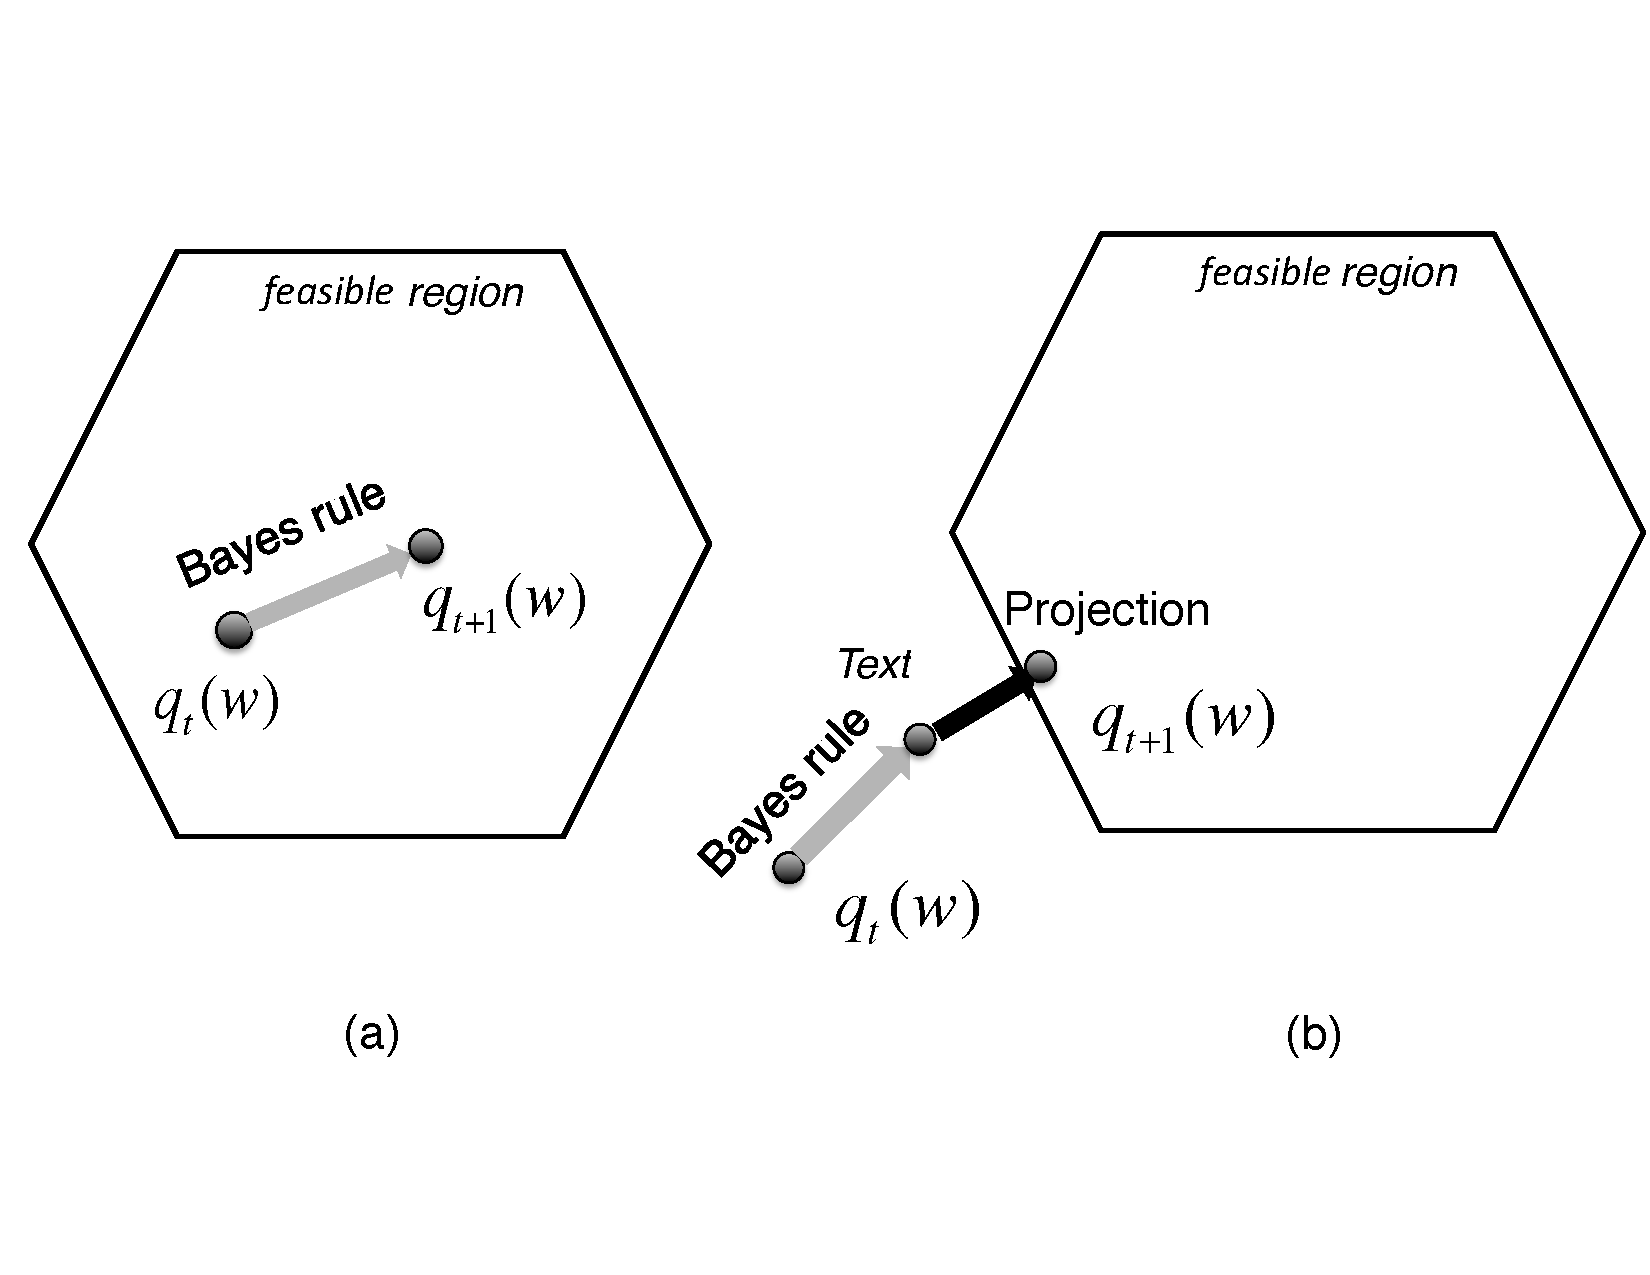
\includegraphics[width=0.7\textwidth]{pa.pdf}
\end{center}\vspace{-.3cm}
\caption{Graphical Illustration of BayesPA learning. \textbf{(a)}. Update \emph{passively} by Bayes rule, if the resulting distribution suffer zero loss. \textbf{(b)} Otherwise, \emph{aggressively} project the resulting distribution to the feasible zone of weights with zero loss. }\label{fig:bayesPA}\vspace{-.3cm}
\end{figure}

\subsection{Online BayesPA Learning}
%We generalize online PA learning to the Bayesian setting.
Instead of updating a point estimate of $\bm{w}$, online Bayesian PA (BayesPA) sequentially infers a new post-data posterior distribution $q_{t+1}(\bm{w})$, either parametric or nonparametric, on the arrival of new data $(\xv_t, y_t)$ by solving the following optimization problem:
%Classification problems are considered in this paper. Specifically, the following update rule is considered:
\setlength\arraycolsep{1pt} \begin{equation}\label{eq:onlinepa}
\begin{array}{rl}
\underset{q(\bm{w}) \in \mathcal{F}_t}{\operatorname{min}} & ~\KL\Big[q(\bm{w}) || q_{t}(\bm{w}) \Big]-\mathbb{E}_{q(\bm{w})}\Big[\log p(\bm{x}_t | \bm{w})\Big] \\
\text{s.t.:} &~~ \ell_\epsilon\Big(q(\bm{w}); \bm{x}_t, y_t\Big) = 0,
\end{array}
\end{equation}
where $\mathcal{F}_t$ can be some family of distributions or the probability simplex $\prob$. For convenience, we denote the objective as $\mathcal{L}(q(\wv))$. In words, we find a post-data posterior distribution $q_{t+1}(\bm{w})$ in the feasible zone that is not only close to $q_t(\bm{w})$ in terms of KL-divergence, but also has a high likelihood of explaining new data. %Notice that the likelihood term is peculiar to the Bayesian setting.
As a result, if Bayes' rule already gives the posterior distribution $q_{t+1}(\bm{w}) \propto q_{t}(\bm{w}) p(\bm{x}_t | \bm{w})$ that suffers no loss (i.e., $\ell_\epsilon = 0$), BayesPA \emph{passively} updates the posterior following just Bayes' rule;\footnote{Under the Bayesian setting, we regard Bayes' rule as a natural update (passive), since no aggressive projection is applied.} otherwise, BayesPA \emph{aggressively} projects the new posterior to the feasible zone of posteriors that attain zero loss. The passive and aggressive update cases are illustrated in Figure~\ref{fig:bayesPA}. We should note that when no likelihood is defined (e.g., $p(\xv_t|\wv)$ is independent of $\wv$), BayesPA will passively set $q_{t+1}(\wv) = q_t(\wv)$ if $q_t(\wv)$ suffers no loss; otherwise, it will aggressively project $q_t(\wv)$ to the feasible zone. We call it {\it non-likelihood} BayesPA.

In practical problems, the constraints in (\ref{eq:onlinepa}) could be unrealizable. To deal with such cases, we introduce the soft-margin version of BayesPA learning, which is equivalent to minimizing the objective function $\mathcal{L}(q(\bm{w}))$ in problem (\ref{eq:onlinepa}) with a regularization term \citep{cortes1995support}:
\setlength\arraycolsep{-3pt}\begin{eqnarray}\label{eq:onlinepa_reg}
&&q_{t+1}(\bm{w}) = \underset{q(\bm{w}) \in \mathcal{F}_t}{\operatorname{argmin}} ~\mathcal{L}\Big(q(\bm{w})\Big) + 2c \cdot \ell_\epsilon\Big(q(\bm{w}); \bm{x}_t, y_t\Big).
\end{eqnarray}
%
% and $c$ is a parameter controlling the extent of regularization.
For the max-margin classifiers that we consider, two types of loss functionals $\ell_\epsilon(q(\bm{w}); \bm{x}_t, y_t)$ are common:
\begin{enumerate}
\item {\bf Averaging classifier}: assume that a post-data posterior distribution $q(\wv)$ is given, then an averaging classifier makes predictions using the sign rule $\hat{y}_t = \textrm{sign} ~ \mathbb{E}_{q(\bm{w})}[\bm{w}^\top \bm{x}_t]$ when the discriminant function has the simple linear form, $f(\xv_t; \wv) = \wv^\top \xv_t$. For this classifier, its hinge loss is therefore defined as:
\setlength\arraycolsep{1pt}\begin{equation*}
%\label{eq:bayes_loss}
\ell_\epsilon^\text{ave}\Big(q(\bm{w}); \bm{x}_t, y_t\Big) = \left(\epsilon-y_t \mathbb{E}_{q(\bm{w})}\left[\bm{w}^\top \bm{x}_t\right]\right)_+ .
\end{equation*}
\item {\bf Gibbs classifier}: assume that a post-data posterior distribution $q(\wv)$ is given, then a Gibbs classifier randomly draws a weight vector $\bm{w} \sim q(\bm{w})$ to make predictions using the sign rule $\hat{y}_t = \textrm{sign}~\bm{w}^\top \bm{x}_t$, when the discrimant function has the same linear form. For each single $\wv$, we can measure its hinge loss $(\epsilon-y_t \bm{w}^\top \bm{x}_t )_+$. To account for the randomness of $\wv$, the expected hinge loss of a Gibbs classifier is therefore defined as:

\begin{equation*}
%\label{eq:gibbs_loss}
\ell_\epsilon^{\text{gibbs}}\Big(q(\bm{w}); \bm{x}_t, y_t\Big) = \mathbb{E}_{q(\bm{w})}\left[ \left( \epsilon-y_t \bm{w}^\top \bm{x}_t \right)_+\right].
\end{equation*}
\end{enumerate}
They are closely connected via the following lemma due to the convexity of the function $(x)_+$.
\begin{lemma}\label{lm:loss}
The expected hinge loss $\ell_\epsilon^{\text{gibbs}}$ is an upper bound of the hinge loss $\ell_\epsilon^{\text{ave}}$, that is, $$\ell_\epsilon^{\text{gibbs}}\Big(q(\bm{w}); \bm{x}_t, y_t\Big) \geq \ell_\epsilon^{\text{ave}}\Big(q(\bm{w}); \bm{x}_t, y_t\Big).$$
\end{lemma}

BayesPA is deeply connected to its various precursors reviewed in Section~\ref{sec:pre}, as summarized in Table~\ref{table:relationship}. First, BayesPA is a natural Bayesian extension of online PA, which is explicated via the following theorem. Note that this theorem only serves as a connection to PA, and will not be relied on by our algorithms, where we are more interested in the cases with nontrivial likelihood models to describe the underlying structures (e.g., topic structures), which are typically out-of-reach for the standard PA. Nevertheless, the idea of the proof details would later be applied to develop practical BayesPA algorithms for topic models. Therefore, we include the complete proof here.

\begin{table*}[t]
\centering
%\setlength\tabcolsep{1pt}
\begin{tabular}{
%!{\vrule width.5pt}
c|c|c|c}
%!{\vrule width.5pt}}
%\Xhline{1.2pt}
\hline\hline
 \textbf{Methods} & Max-margin learning ? & Bayesian inference ? & Streaming update ? \\
\hline
PA & yes & no  &  yes  \\
SVB & no & yes  &  yes  \\
RegBayes & yes & yes & no \\
BayesPA & yes & yes & yes \\
\hline\hline
\end{tabular}
\caption{The comparison between BayesPA and its various precursors, including online PA, streaming variational Bayes (SVB) and regularized Bayesian inference (RegBayes), in three different aspects.}\label{table:relationship}\vspace{-0.3cm}
\end{table*}

\begin{theorem} \label{tm:subsume}
If $q_0(\bm{w}) = \mathcal{N}(0, I)$, $\mathcal{F}_t=\prob$, the likelihood is constant and we use the averaging classifier $\ell_\epsilon^\text{ave}$, the non-likelihood BayesPA subsumes the online PA.
\end{theorem}


%
\begin{proof}
The soft-margin version of BayesPA learning can be reformulated using a slack variable $\xi_t$:
\setlength\arraycolsep{1pt} \begin{equation}\label{eq:onlinepa_reg_app}
\begin{array}{ccc}
& q_{t+1}(\bm{w}) = & \underset{q(\bm{w}) \in \mathcal{P}}{\operatorname{argmin}} ~\text{KL}\Big[ q(\wv) || q_t(\wv) \Big] + 2 c \cdot \xi_t \\
&& \text{s.t.}: y_t \mathbb{E}_{q(\wv)}\left[ {\wv}^\top \xv_t \right] \geq \epsilon-\xi_t, ~~ \xi_t \geq 0.
\end{array}
\end{equation}
Similar to Corollary 5 in \citep{zhu2012medlda}, the optimal solution $q^*(\wv)$ of the above problem can be derived from its functional Lagrangian  and has the following form:
\begin{equation}
\label{eq:optimal}
q^*(\wv) = \frac{1}{\Gamma(\tau_t^*, \xv_t, y_t)} q_t(\wv) \exp\Big( \tau_t^* y_t \wv^\top \xv_t \Big),
\end{equation}
where the normalization term $\Gamma(\tau_t, \xv_t, y_t) = \int_{\wv}{q_t(\wv) \exp\Big(\tau_t y_t \wv^\top \xv_t \Big)d\wv}$, and $\tau_t^*$ is the optimal solution to the dual problem
\begin{equation}
\begin{array}{rl}
\label{eq:dual}
\max\limits_{\tau_t} & {~\epsilon\tau_t-\log \Gamma(\tau_t, \xv_t, y_t)} \\
\text{s.t.: } &  0 \leq \tau_t \leq 2 c .
\end{array}
\end{equation}
Using this primal-dual interpretation, we prove that for the normal prior $p_0(\bm{w}) = \mathcal{N}(\bm{w}_0, I)$, the post-data posterior is also Gaussian: $q_t(\bm{w}) = \mathcal{N}(\muv_t, I)$ for some $\muv_t$ in each round $t = 0, 1, 2, ...$ This can be shown by induction. By our assumption, $q_0(\wv) = p_0(\wv) = \normal(\wv_0, I)$ is Gaussian. Assume for round $t \geq 0$, the distribution $q_{t}(\wv) = \mathcal{N}(\muv_{t}, I)$. Then for round $t+1$, Eq.~(\ref{eq:optimal}) suggests the distribution
\begin{equation*}
q_{t+1}(\wv) = \frac{\mathcal{C}}{\Gamma(\tau_t^*, \xv_t, y_t)} \exp\left( -\frac{1}{2} ||\wv-(\muv_t+\tau_t^* y_t \xv_t)||^2 \right),
\end{equation*}
where the constant $\mathcal{C} = \exp(y_t \tau_t^* \muv_t^\top \xv_t  + \frac{1}{2} \tau_t^{*2} \xv_t^\top \xv_t)$ . Therefore, the distribution $q_{t+1}(\wv) = \mathcal{N}(\muv_t + \tau_t^* y_t \xv_t, I)$, and the normalization term is $\Gamma(\tau_t, \xv_t, y_t) = (\sqrt{2 \pi})^K \exp(\tau_t y_t \xv_t^\top \muv_t+\frac{1}{2} \tau_t^{2} \xv_t^\top \xv_t)$ for any $\tau_t \in [0, 2c]$.

Next, we show that $\muv_{t+1} = \muv_{t}+\tau_t^* y_t \xv_t$ is the optimal solution of the online PA update rule \citep{crammer2006pa}. To see this, we replace $\Gamma(\tau_t, \xv_t, y_t)$ in problem (\ref{eq:dual}) with our derived form. Ignoring constant terms, we obtain the dual problem
\begin{equation}
\begin{array}{rl}
\label{eq:dualx}
\max\limits_{\tau_t}& {~\epsilon \tau_t-\frac{1}{2}\tau_t^2 \xv_t^\top \xv_t- y_t \tau_t \muv_t^\top \xv_t} \\
\text{s.t.: }&  0 \leq \tau_t \leq 2 c ,
\end{array}
\end{equation}
which is exactly the dual form of the online PA update equation:
\begin{equation*}
\begin{array}{rl}
\muv_{t+1}^{\text{PA}} = & \arg\min\limits_{\muv}{~ \frac{1}{2} ||\muv-\muv_{t}||^2+2 c \cdot \xi_t } \\
\text{s.t.   }  & y_t \muv^\top \xv_t \geq \epsilon-\xi_t, ~~ \xi_t \geq 0.
\end{array}
\end{equation*}
The optimal solution is $\muv_{t+1}^{\text{PA}} = \muv_{t}+\tau_t^* y_t \xv_t$. Note that $\tau_t^*$ is the optimal solution of dual problem (\ref{eq:dualx}) shared by both PA and BayesPA. Therefore, we conclude that  $\muv_{t+1} = \muv_{t+1}^{\text{PA}}$.
\end{proof}



%online BayesPA essentially defines a streaming update rule for RegBayes when the posterior constraints are derived from the max-margin principle; BayesPA is a Bayesian generalization of online PA; and BayesPA augments the streaming variational Bayes (SVB) by imposing max-margin posterior constraints, where the variational treatment of BayesPA will be clear soon later though alternative inference methods (e.g., Monte Carlo) may exist.
%

%BayesPA is deeply connected to the preliminary topics discussed in section \ref{sec:pre}.
%
Second, suppose some algorithm $\algo$ is capable of solving problem~(\ref{eq:onlinepa_reg}), then it would produce streaming updates to the posterior distribution. For averaging classifiers, it is easy to modify the proof of theorem \ref{tm:subsume} to derive the update rule of BayesPA, which is be presented in the following lemma.
%
\begin{lemma}\label{lemma:avgBayesPA-Rep}
If $\mathcal{F}_t=\prob$ and we use the averaging classifier with loss functional $\ell_\epsilon^\text{ave}$, the update rule of online BayesPA is
%
\begin{equation}\label{eq:avgBayesPA-optimal}
q_{t+1}(\wv) = \frac{1}{\Gamma(\tau_t^*, \xv_t, y_t)} q_t(\wv) p(\xv_t | \wv) \exp\Big(\tau_t^* y_t \wv^\top \xv_t \Big),
\end{equation}
where $\Gamma(\tau_t, \xv_t, y_t)$ is the normalization term
$%\begin{equation*}
\Gamma(\tau_t, \xv_t, y_t) = \int_{\wv}{q_t(\wv) p(\xv_t | \wv) \exp \Big(\tau_t y_t \wv_t^\top \xv_t \Big)d\wv},
$ %\end{equation*}
and $\tau_t^*$ is the optimal solution to the dual problem
\textnormal{\begin{equation} \nonumber
\begin{array}{rl}
\max\limits_{\tau_t} & ~~~~~~~~~ {~\epsilon\tau_t-\log \Gamma(\tau_t, \xv_t, y_t)} \\
\text{s.t. } & ~~~~~~~~~ 0 \leq \tau_t \leq 2 c .
\end{array}
\end{equation}}
\end{lemma}
For Gibbs classifiers, we have the following lemma to characterize its streaming update rule.
\begin{lemma} \label{lm:pagibbs}
If $\mathcal{F}_t=\prob$ and we use the Gibbs classifier with loss functional  $\ell_\epsilon^{\text{gibbs}}$, the update rule of online BayesPA is
%
\begin{equation}\label{eq:onlinepa_gibbs}
q_{t+1}(\wv) = \frac{q_{t}(\wv) p(\xv_t | \wv) \exp\left( - 2 c \left( \epsilon-y_t \wv^\top \xv_t \right)_+ \right) }{\Gamma(\xv_t, y_t)},
\end{equation}
%
where $\Gamma(\xv_t, y_t)$ is the normalization constant.
\end{lemma}
In both update rules (\ref{eq:avgBayesPA-optimal}) and (\ref{eq:onlinepa_gibbs}), the post-data posterior $q_t(\bm{w})$ in the previous round $t$ can be treated as a prior, while the newly observed data and the loss it incurs provide a likelihood and an un-normalized pseudo-likelihood respectively. Due to the analytical form, the BayesPA update rule~(\ref{eq:onlinepa_gibbs}) is sequential in nature, simiar as the convential Bayes rule~(\ref{eq:stream-Bayes-update}). Therefore, the sequential posterior at time $T$ is the same as the batch posterior that observes all the data instances up to $T$.
For the case with averaging classifers, Eq.~(\ref{eq:avgBayesPA-optimal}) reduces to the streaming Bayesian update problem if there is no loss functional (i.e., $\ell_\epsilon = 0$). Therefore, BayesPA is an extension to streaming variational Bayes (SVB) with imposed max-margin posterior constraints.

Finally, the update formulation~(\ref{eq:onlinepa_reg}) is essentially a RegBayes problem with a single data point $(\xv_t, y_t)$. Although RegBayes inference is normally intractable, we would show later in the paper how to use variational approximation to bypass the difficulty for specific settings. This would lead to variational approximation algorithm $\algo$ for the streaming update of post-data posterior.

Besides treating a single data point at a time, a useful technique in practice to reduce the noise in data is to use mini-batches. Suppose that we have a mini-batch of data points at time $t$ with an index set $B_t$. Let $\Xv_t = \{\xv_d\}_{d \in B_t}, \Yv_t = \{y_{d}\}_{d \in B_t}$. The online BayesPA update equation for this mini-batch can be defined in a natural way:
%
\begin{equation*} %\label{eq:bayespa_latent_batch}
\underset{q \in \mathcal{F}_t}{\operatorname{min}}{~ ~\KL\Big[q(\bm{w}) || q_{t}(\bm{w}) \Big]-\mathbb{E}_{q(\bm{w})}\Big[\log p(\Xv_t | \bm{w})\Big] + 2c \cdot \ell_\epsilon\Big(q(\wv); \Xv_t, \Yv_t\Big)},
\end{equation*}
%
where $\ell_\epsilon(q(\wv); \Xv_t, \Yv_t) = \sum_{d \in B_t}{\ell_\epsilon(q(\wv); \xv_d, y_d)}$. Like PA methods~\citep{crammer2006pa}, BayesPA on mini-batches may not have closed-form update rules, and numerical optimization methods are needed to solve this new formulation.

\subsection{BayesPA Learning with Latent Structures}\label{sec:pa_latent}

\begin{figure}
\begin{center}
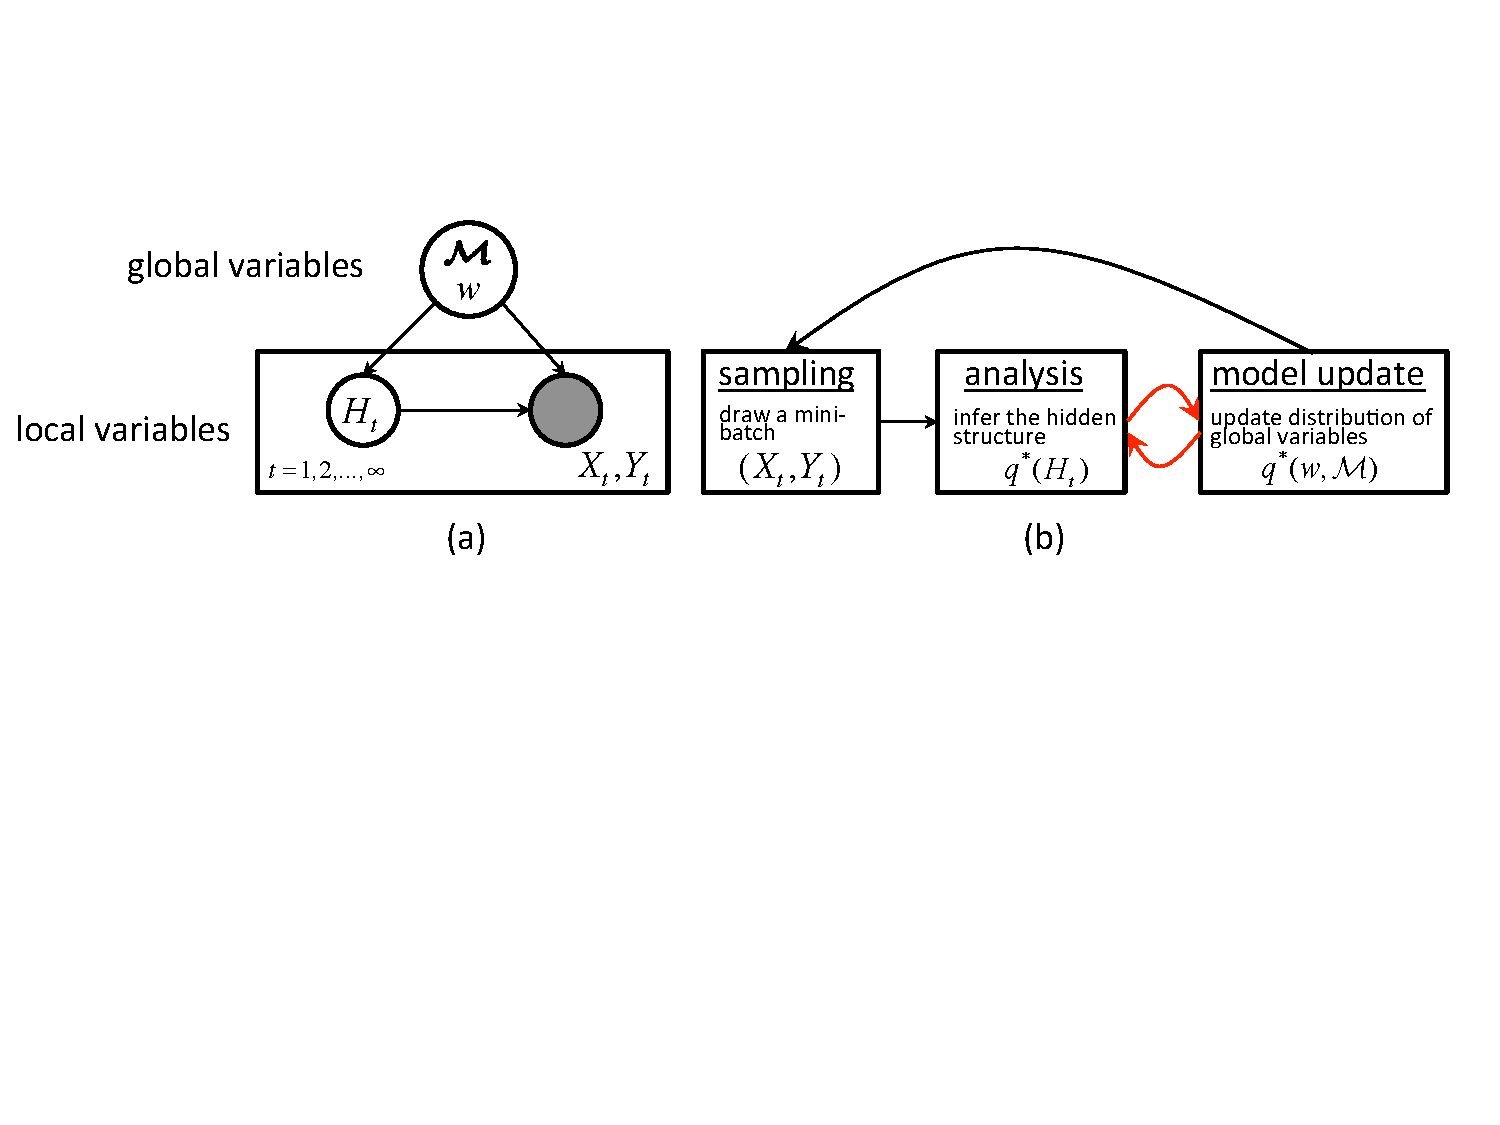
\includegraphics[width=\textwidth]{graph.pdf}
\end{center}\vspace{-.4cm}
\caption{Graphical illustrations of: (a) the abstraction of models with latent structures; and (b) the procedure of BayesPA learning with latent structures.}\label{fig:LatentBayesPA}\vspace{-.4cm}
\end{figure}

To expressively explain complex real-word data, Bayesian models with latent structures have been extensively developed. The latent structures could typically be characterized by a hierarchy of  variables, which are generally grouped into two sets---\emph{local latent variables} $\hv_d$ ($d \geq 0$) that characterize the hidden structures of each observed data $\xv_d$ and \emph{global variables} $\Mv$ that capture the common properties shared by all data.

As illustrated in Figure~\ref{fig:LatentBayesPA}, BayesPA learning with latent structures aims to update the distribution of $\Mv$ as well as the classifier weights $\wv$, based on each incoming mini-batch $(\Xv_t, \Yv_t)$ and their corresponding latent variables $\Hv_t = \{\hv_d\}_{d \in B_t}$. Because of the uncertainty in $\Hv_t$, our posterior approximation algorithm $\algo$ would first infer the joint posterior distribution $q_{t+1}(\wv, \Mv, \Hv_t)$ from
\begin{eqnarray}\label{eq:bayespa_latent}
\underset{q \in \mathcal{F}_t}{\operatorname{min}}{~\mathcal{L}\Big( q(\wv, \Mv, \Hv_t) \Big) + 2 c \cdot \ell_\epsilon\Big( q(\wv, \Mv, \Hv_t); \Xv_t, \Yv_t \Big)},
\end{eqnarray}
where $\mathcal{L}(q) =  \text{KL}[q(\wv, \Mv, \Hv_t) ||  q_t(\wv, \Mv) p_0(\Hv_t)] -\mathbb{E}_{q(\wv, \Mv, \Hv_t)}[\log p(\Xv_t | \wv,  \Mv, \Hv_t)]$ and $\ell_\epsilon(q(\wv, \Mv, \Hv_t); \Xv_t, \Yv_t)$ is some cumulative loss functional on the min-batch data incurred by some classifiers on the latent variables $\Hv_t$ and/or global variables $\Mv$. As in the case without latent variables, both averaging classifier and Gibbs classifier can be used.

%To see the connection of (\ref{eq:bayespa_latent}) to (\ref{eq:onlinepa}), let the latent variables $\Hv_t$ be fully observed, which implies the space of $\Hv_t$ is collapsed to a point. In that case, (\ref{eq:bayespa_latent}) and (\ref{eq:onlinepa}) become equivalent just by a substitution of global variables.

%  The data likelihood is
%
%\begin{equation}
%\Pr[\bm{X}_t | \bm{w}] = \int_{\bm{Z}_t}{\Pr[\bm{X}_t, \bm{Z}_t | \bm{w}] d \bm{Z}_t}
%\end{equation}¥
%
%for continuos variables $\bm{Z}_t$, and for discrete $\bm{Z}_t$ as well, if the integral is replaced by summation. On the other hand, the loss function $\ell_\epsilon(q(\bm{\mathcal{M}}, \bm{w}); \bm{Z}_t, y_t)$ is now defined with respect to latent variables.

In the sequel, algorithm $\algo$ produces the approximate posterior $q_{t+1}(\wv, \Mv)$. In general we would not obtain a closed-form posterior distribution by marginalizing out $\Hv_t$, especially in dealing with some involved models like MedLDA \citep{zhu2012medlda}. The intractability is bypassed through the mean-field assumption $q(\wv, \Mv, \Hv_t) = q(\wv) q(\Mv) q(\Hv_t)$. Specifically, algorithm $\algo$ solves problem~(\ref{eq:bayespa_latent}) using an iterative procedure and obtain the optimal distribution $q^*(\wv) q^*(\Mv) q^*(\Hv_t)$. Then it sets $q_{t+1}(\wv, \Mv) = q^*(\wv) q^*(\Mv)$ and proceeds to next round. Concrete examples of this method will be discussed in Section \ref{sec:pamedlda} and Section \ref{sec:extensions}.
%Before diving into the details, we should note that in real online setting, only global variables are maintained in the bookkeeping, while the local information in the streaming data is forgotten. However, problem~(\ref{eq:bayespa_latent}) gives us a distribution of $(\wv, \Mv)$ that is coupled with the local variables $\Hv_t$.
%Although in some cases we can marginalize out the local variables $\Hv_t$, in general we would not obtain a closed-form posterior distribution $q_{t+1}(\wv, \Mv)$ for the next optimization round, especially in dealing with some involved models like MedLDA \citep{zhu2012medlda}. Therefore, we resort to approximation methods, e.g., by posing additional assumptions about $q(\wv, \Mv, \Hv_t)$ such as the mean-field assumption, $q(\wv, \Mv, \Hv_t) = q(\wv) q(\Mv) q(\Hv_t)$. Then, we can solve the problem via an iterative procedure and use the optimal distribution $q^*(\wv) q^*(\Mv)$ as $q_{t+1}(\wv, \Mv)$. More details will be provided in next sections.

\iffalse
\begin{algorithm}[t]
\caption{\small{Variational Passive-Aggressive Inference}}\label{algo:var_pa}
\begin{algorithmic}[1]
\STATE Let $q_0(\Mv, \wv) = p_0(\Mv, \wv)$ be the prior.
\FOR{$t = 1 \to \infty$}
\STATE Let $\mathcal{F}_t = \{q ~|~ q(\Mv, \wv, \Hv_t)=q(\Mv)(\wv)(\Hv_t)\}$
\STATE Find $q^*(\Mv)q^*(\wv)q^*(\Hv_t) \in \mathcal{F}_t$ that minimizes~(\ref{eq:bayespa_latent}). %\\ \small{$\mathcal{L}(q(\bm{\mathcal{M}})q( \bm{w})q( \bm{Z}_t))+c \ell_\epsilon(q(\bm{\mathcal{M}})q( \bm{w})q( \bm{Z}_t); \bm{X}_t, \bm{Y}_t)$}.
\STATE Update $q_{t+1}(\Mv, \wv) = q^*(\Mv)q^*(\wv)$.
\ENDFOR
\end{algorithmic}
\end{algorithm}
\fi

%For topic models, it is not rare that data likelihood has a conjugate distribution family. Therefore, as we shall see in Section \ref{sec:otm} and \ref{sec:ohdp}, the mean-field assumption leads to efficient online learning algorithms for these topic models, while the accuracy tradeoff is kept minimum.

\iffalse
Besides, because of the possibly rich structure in $\Hv_t$, the loss function $\ell_\epsilon$ in (\ref{eq:bayespa_latent}) is generally amorphous, depending on how the prediction rule is defined. A specific class of prediction rules commonly used is latent linear discriminant function \citep{zhu2012medlda}:
\begin{equation} \label{eq:latent_discriminant}
f(\wv, \Hv_t) = \wv^\top f(\Hv_t)
\end{equation}
where $f(\cdot)$ is a feature function mapping from the space of latent structure to the space of real vectors. In the following section, we illustrate that efficient inference algorithms can be developed with (\ref{eq:latent_discriminant}) using the mean-field assumption. In fact, we can show that for averaging classifiers and $q_0(\bm{w}) = \mathcal{N}(0, I)$,  the mean of $q^*(\wv)$ is updated just by the online PA rule (\ref{eq:pa-soft}). However, as in online PA, it is hard to derive a close-form update rule for this approach when dealing with mini-batches. Nevertheless, we illustrate that the power of BayesPA could extend further, as we develop fast online algorithms for topic models using Gibbs classifiers.
\fi

%\eat
{

\section{Theoretical Analysis}\label{sec:theory}

In this section, we provide theoretical analysis for BayesPA learning. We consider the fully observed case where no latent structures are assumed, and leave the more complex case with hidden structures as future work. Specifically, we prove \emph{regret bounds}~\citep{murphy2012machine_reget,shalev2006convex}, which relate the cumulative loss attained by our algorithms on \emph{any} sequence of incoming samples to that by a fixed distribution of models $p(\wv)$. Such bounds guarantee that the loss $\ell_\epsilon$ of the online learning algorithms cannot be too much larger compared to the loss $\ell^*_\epsilon$ of any fixed predictor chosen with hindsight of all data.

\eat{
\begin{definition}
\textbf{(Bayesian Regret)} Let $(\xv_0, y_0)$, $...$, $(\xv_{T-1}, y_{T-1})$ be a sequence of incoming data where $\xv_t \in \mathbb{R}^K$ and $y_t \in \{-1, 1\}$. The Bayesian Regret of online Bayesian learning with both likelihood function $p(\xv | \wv)$ and loss function $\ell_\epsilon(q(\wv); \xv, y)$ is defined as
\begin{equation}
\regret_T(q(\wv)) = \sum\limits_{t=0}^{T-1}{\ell_\epsilon(q_t(\wv | \xv_t); \xv_t, y_t)}
\end{equation}
where $q_t(\wv | \xv_t) \propto q_t(\wv) p(\xv | \wv)$ is the posterior from observing $\xv_t$. We use the notation $\regret_T^\text{ave}$ for $\ell_\epsilon^\text{ave}$ and $\regret_T^\text{gibbs}$ for $\ell_\epsilon^\text{gibbs}$.
\end{definition}

In other words, the regret is incurred cumulatively round by round: At the beginning of each round, the algorithm observes $\xv_t$, updates its belief about $\wv$ via the Bayes' rule, and makes a decision; the decision then incurs loss at the end of each round via $\ell_\epsilon(q(\wv); \xv_t, y_t)$. Note that for non-likelihood BayesPA, the Bayesian regret reduces to the typical notion of regret. }

In BayesPA learning, however, not only do we desire a model $\wv$ with low cumulative loss, we also want $\wv$ to have high cumulative likelihood. To capture this fact, we generalize the notion of regret as follows.

\begin{definition}
\textbf{(Bayesian Regret)} The Bayesian Regret at observing $(\xv_t, y_t)$ with the current model $q(\wv)$ is defined as
\begin{equation}
\mathcal{R}_c(q(\wv); \xv_t, y_t) = -\ep_{q(\wv)}[\log p(\xv_t | \wv)]+2 c \cdot \ell_\epsilon(q(\wv_t); \xv_t, y_t)
\end{equation}
where $c$ is a parameter determining the trade-off between likelihood and loss, characterized by some loss function $\ell_\epsilon(q(\wv_t); \xv_t, y_t)$.
\end{definition}
We will use the notation $\regret_c^\text{ave}$ for the Bayesian regret if choosing the averaging loss $\ell_\epsilon^\text{ave}$ and use the notation $\regret_c^\text{gibbs}$ if choosing the Gibbs loss $\ell_\epsilon^\text{gibbs}$. For non-likelihood BayesPA, the regret is naturally reduced to be $\mathcal{R}_c(q(\wv); \xv_t, y_t) = \ell_\epsilon(q(\wv_t); \xv_t, y_t)$. Our below analysis considers the full BayesPA. The main results are applicable for non-likelihood BayesPA, as remarked later.

\begin{theorem}[A regret bound for BayesPA with Gibbs classifiers]\label{tm:gibbs-new}
Let the initial prior be $q_0(\wv)$. For any fixed distribution $p(\wv)$ and any $\beta \in (0,1)$, the regret of BayesPA is bounded as
\textnormal{ \setlength\arraycolsep{1pt} \begin{eqnarray} \label{eq:gibbsnlpa_bound-new}
(1-\beta) \sum\limits_{t=0}^{T-1}{\regret_c^\text{gibbs}(q_t(\wv); \xv_t, y_t)} \leq \log (\frac{1}{\beta}) \sum\limits_{t=0}^{T-1}{\regret_c^\text{gibbs}(p(\wv); \xv_t, y_t)}+\KL[p(\wv)||p_0(\wv)].  \end{eqnarray}}
\end{theorem}
\begin{proof}
According to Lemma \ref{lm:pagibbs}, the update rule for the distribution $q(\wv)$ is
\begin{equation*}
q_{t+1}(\wv) = \frac{1}{\Gamma(\xv_t, y_t)} q_t(\wv) p(\xv_t | \wv) e^{-2c \left(\epsilon-y_t \wv^\top \xv_t\right)_{+}},
\end{equation*}
where $\Gamma(\xv_t, y_t)$ is the partition function
$\Gamma(\xv_t, y_t) = \int_{\wv}{q_{t}(\wv) p(\xv_t | \wv)e^{-2 c \left(\epsilon-y_t \wv^\top \xv_t\right)_{+}} d \wv}$.
Let $\ell_\epsilon(\wv; \xv_t, y_t) = -\log p(\xv_t | \wv) + 2c \left(\epsilon-y_t \wv^\top \xv_t\right)_{+}$ be the log-loss at iteration $t$ on receiving $\xv_t$. Then, we can apply the log-loss bound~\citep[Theorem 3]{bayes-bounds} to show the results.
\end{proof}\vspace{-.5cm}
\begin{remark}
The bound (\ref{eq:gibbsnlpa_bound-new}) implies that the regret satisfies $$\frac{1}{T} \sum_{t=0}^{T-1}{\regret_c(q_t(\wv); \xv_t, y_t)} \leq  \frac{\log 1/ \beta}{T(1-\beta)}\sum_{t=0}^{T-1}{\regret_c(p(\wv); \xv_t, y_t)} + \frac{1}{T (1-\beta)} \KL[p(\wv) || q_0(\wv)].$$
With proper choice of $\beta$, for example $1-\beta = 1/\sqrt{T}$, we can have $\frac{\log(1/\beta)}{1-\beta} \rightarrow 1$ and $\frac{1}{T(1-\beta)} \rightarrow 0$. So the asymptotic average regret of BayesPA with Gibbs classifiers vanishes as $T \rightarrow \infty$
\end{remark}

Below, we analyze the regret bound for BayesPA with an averaging classifier, whose bound is unfortunately looser due to the technical difficulty that we do not have an analytical update rule at each iteration.

\iffalse
\begin{theorem}[A regret bound for BayesPA with Gibbs classifiers]\label{tm:gibbs}
Let the initial prior be $q_0(\wv)$. For all $t \in \{0,1,...,T-1\}$, define the  exponential family of tilted distributions
 \[\allowbreak q_{t, \tau}(\wv) \propto  q_{t}(\wv) \exp(\tau \mathcal{T}(\wv, \xv_t, y_t))\]
 with parameter $\tau$ and sufficient statistics
 \begin{equation*}
 \mathcal{T}(\wv, \xv_t, y_t) = -\log p(\xv_t | \wv)+\frac{1}{2c}(\epsilon-y_t \wv^\top \xv_t)_{+}.
 \end{equation*}
If the Fisher information of $\mathcal{T}(\wv, \xv_t, y_t)$ about $\tau$ satisfies
\textnormal{\begin{equation}
 J_{\mathcal{T}(\wv, \xv_t, y_t)}(\tau) = \var_{q_{t, \tau}(\wv)}\left[ \mathcal{T}(\wv, \xv_t, y_t)\right] \leq R
\end{equation}}
 for all parameters $0 < \tau < 2 c$ and some constant $R > 0$. Then for any fixed distribution $p(\wv)$, the regret of BayesPA is bounded as
\textnormal{ \setlength\arraycolsep{1pt} \begin{eqnarray} \label{eq:gibbsnlpa_bound}
\sum\limits_{t=0}^{T-1}{\regret_c^\text{gibbs}(q_t(\wv); \xv_t, y_t)} \leq \sum\limits_{t=0}^{T-1}{\regret_c^\text{gibbs}(p(\wv); \xv_t, y_t)}+\KL[p(\wv)||p_0(\wv)]+ 2 c^2 R T.  \end{eqnarray}}
\end{theorem}

\begin{proof}
According to Lemma \ref{lm:pagibbs}, the update rule for the distribution $q(\wv)$ is
\begin{equation*}
q_{t+1}(\wv) = \frac{1}{\Gamma(\xv_t, y_t)} q_t(\wv) p(\xv_t | \wv) e^{-2c \left(\epsilon-y_t \wv^\top \xv_t\right)_{+}},
\end{equation*}
where $\Gamma(\xv_t, y_t)$ is the partition function
\begin{equation*}
\Gamma(\xv_t, y_t) = \int_{\wv}{q_{t}(\wv) p(\xv_t | \wv)e^{-2 c \left(\epsilon-y_t \wv^\top \xv_t\right)_{+}} d \wv}.
\end{equation*}
The proof idea is to relate the loss $\ell^\text{gibbs}_{\epsilon}(\xv_t)$ in each round with the difference of prior $q_t(\wv)$ and posterior $q_{t+1}(\wv)$, which is
\eat{\begin{equation} \label{eq:kl_diff_gibbs}
\KL[p || q_{t}]-\KL[p || q_{t+1}]  = \ep_{p(\wv)}[\log p(\xv_t | \wv)]-2 c \cdot \ell^\text{gibbs}_\epsilon(p(\wv); \xv_t, y_t)-\log \Gamma(\xv_t, y_t).
\end{equation}}
\begin{equation} \label{eq:kl_diff_gibbs}
\KL[p(\wv) || q_{t}(\wv)]-\KL[p(\wv) || q_{t+1}(\wv)]  = -\regret_c^\text{gibbs}(p(\wv); \xv_t, y_t) - \log \Gamma(\xv_t, y_t).
\end{equation}
\junx{how about starting from here and using the equality that $KL(q_t \Vert q_{t+1}) = \log \Gamma(\xv_t, y_t) + R_c^{gibbs}(q_t; \xv_t, y_t)$? Then, we can get $\sum_t R_c(q_t) \leq \sum_t R_c(p) + KL(p \Vert p_0) + \sum_t KL(q_t \Vert q_{t+1})$. If the sequence $q_t$ converges (which is true with some proper conditions), then the last term should be sublinear to $T$, right?}
Construct a canonical exponential family $q_{t,\tau}(\wv)$ parameterized by $\tau$ through tilting the base distribution $q_t(\wv)$ as follows:
\begin{equation*}
q_{t,\tau}(\wv) = q_{t}(\wv) \exp\Big(\frac{\tau}{2c} (\log p(\xv_t | \wv)-2c (\epsilon-y_t \wv^\top \xv_t)_{+})-\log f(\tau)\Big),
\end{equation*}
where the log partition function
\begin{equation*}
\log  f(\tau) = \log\left( \int_{\wv}{q_{t}(\wv) \Big(p(\xv_t | \wv)^{\frac{1}{2c}} e^{-(\epsilon-y_t \wv^\top \xv_t)_{+} }\Big)^\tau  d \wv} \right).
\end{equation*}
According to properties of exponential family, the first-order and second-order derivatives can be related to its cumulants:
\begin{equation*}
\frac{\partial}{\partial \tau} \log  f(\tau) = \E_{q_{t, \tau}(\wv)}\left[\frac{1}{2c} \log p(\xv_t | \wv) - \left(\epsilon-y_t \wv^\top \xv_t\right)_{+}\right] = -\frac{1}{2c}\regret_c^{gibbs}(q_{t,\tau}(\wv); \xv_t, y_t),
\end{equation*}
\begin{equation*}
\frac{\partial^2}{\partial \tau^2} \log  f(\tau) = \var_{q_{t, \tau}(\wv)}\left[\frac{1}{2c} \log p(\xv_t | \wv)-\left(\epsilon-y_t \wv^\top \xv_t\right)_{+} \right] = J_{\mathcal{T}(\wv, \xv_t, y_t)}(\tau).
\end{equation*}
Using the fact that $\log  f(0) = 0$ and applying Taylor's theorem with the Lagrange's remainder \footnote{The theorem states that if a function $g: \real^k \rightarrow \real$ is $k+1$ times differentiable in a closed ball $B$, then for $\xv_0, \xv \in B$,  $\exists c \in (0,1)$ such that $f(\xv) = f(\xv_0)+\partial f(\xv_0)(\xv-\xv_0)+\frac{1}{2}(\xv-\xv_0)^\top \partial^2 f[c \xv_0+(1-c) \xv] (\xv-\xv_0)$.} at $\tau = 0$, we have a second-order expression
\begin{equation*}
\log  f(\tau) = -\frac{1}{2c}  \regret_c^\text{gibbs}(q_t(\wv); \xv_t, y_t) \tau + \frac{1}{2} J_{\mathcal{T}}(\hat{\tau}) \tau^2,
\end{equation*}
for some $0 \leq \hat{\tau} \leq \tau$. By assumption, $J_{\mathcal{T}}(\hat{\tau})  \leq R$,
\begin{equation*}
\log  f(2c) \leq  - \regret_c^\text{gibbs}(q_t(\wv); \xv_t, y_t) + 2 c^2 R ,
\end{equation*}
Since $\Gamma(\xv_t, y_t) = f(2c)$, Eq.~(\ref{eq:kl_diff_gibbs}) can be lower bounded as
\begin{eqnarray*}
\KL[p(\wv) || q_{t}(\wv)]-\KL[p(\wv) || q_{t+1}(\wv)]  \geq &~~~ -\regret_c^\text{gibbs}(p(\wv); \xv_t, y_t)+\regret_c^\text{gibbs}(q_t(\wv); \xv_t, y_t)-2 c^2 R .
\end{eqnarray*}
Summing over all $t = 0, 1, 2, ..., T-1$ and neglecting $\KL[p(\wv) || q_{T}(\wv)]$, we can obtain (\ref{eq:gibbsnlpa_bound}).
\end{proof}
\fi


%\eat{Notice that by Lemma \ref{lm:loss}, a theoretical guarantee of the BayesPA with averaging classifiers can be trivially derived from Theorem \ref{tm:gibbs}. However, in order to relate their loss directly with the batch averaging classifier, we need the following theorem.}

\begin{theorem}[A regret bound for BayesPA with averaging classifiers]\label{tm:avg}
Let the initial prior be $q_0(\wv)$. For all $t \in {0,1,...,T-1}$, define the expoential family of tilted distributions,
\begin{equation*}
q_{t,\tau, u}(\wv) \propto q_t(\wv) \exp(u \mathcal{U}(\wv, \xv_t, y_t)+\tau \mathcal{T}(\wv, \xv_t, y_t))
\end{equation*}
with two parameters $\tau, u$ and the sufficient statistics,
\begin{eqnarray}
\mathcal{U}(\wv, \xv_t, y_t) = \log p(\xv_t | \wv),~\textrm{and}~\mathcal{T}(\wv, \xv_t, y_t) = y_t \wv^\top \xv_t. \nonumber
\end{eqnarray}
If the Fisher information satisfies,
\begin{equation*}
J_{\mathcal{U}(\wv, \xv_t, y_t)} = \var_{q_{t, \tau, u}}[\mathcal{U}(\wv, \xv_t, y_t)] \leq S, ~~
%\end{equation*}
%and
%\begin{equation*}
J_{\mathcal{T}}(\wv, \xv_t, y_t) = \var_{q_{t,\tau, u}}[\mathcal{T}(\wv, \xv_t, y_t)] \leq R
\end{equation*}
for all $(\tau,u) \in (0,2c) \times (0,1)$.
Then for any fixed distribution $p(\wv)$, the regret of BayesPA satisfies,
\textnormal{ \setlength\arraycolsep{1pt} \begin{eqnarray} \label{eq:avgnlpa_bound}
\sum\limits_{t=0}^{T-1}{\regret_c^\text{ave}(q_t(\wv); \xv_t, y_t)} \leq \sum\limits_{t=0}^{T-1}{\regret_c^\text{ave}(p(\wv); \xv_t, y_t)}+\KL[p(\wv)||p_0(\wv)]+\left( \frac{S}{2}+ 2 c^2 R \right) T.  \end{eqnarray}}
\end{theorem}
\begin{proof}
See Appendix~\ref{app:regret-bound}.
\end{proof}\vspace{-.5cm}

\iffalse
\begin{proof}%\jun{can we defer this proof to appendix to make the main text clear?}
%\strin{I think the proof is important.}
%The proof is similar to that of Gibbs classifiers.
According to Lemma~\ref{lemma:avgBayesPA-Rep}, for BayesPA with averaging classifiers, we have the streaming update rule
\begin{equation*} %\label{eq:sol_bayespa}
q_{t+1}(\wv) = \frac{1}{\Gamma(\tau_t; \xv_t, y_t)} q_t(\wv) p(\xv_t | \wv)e^{\tau_t y_t \wv^\top \xv_t},
\end{equation*}
where $\Gamma(\tau_t; \xv_t, y_t)$ is the partition function and $\tau_t$ is the solution of the dual problem:
\begin{equation} \label{eq:bayespa_dual}
\max\limits_{0 \leq \tau \leq 2c}{\epsilon \tau - \log \Gamma(\tau; \xv_t, y_t)}.
\end{equation}
By definition, the partition function is
$\Gamma(\tau_t; \xv_t, y_t) = \int_{\wv}{q_t(\wv) p(\xv_t|\wv) e^{\tau_t y_t \wv_t \xv_t} d\wv}$. Construct the two parameter exponential family
\begin{equation*}
q_{t,\tau, u}(\wv) = q_t(\wv) \exp\Big(u \log p(\xv_t | \wv)+\tau y_t \wv^\top \xv_t-\log f(\tau, u)\Big),
\end{equation*}
where the log partition function $f(\tau, u)$ is
\begin{equation}
\log f(\tau, u) = \log \int_{\wv}{q_t(\wv) p(\xv_t | \wv)^u e^{\tau y_t \wv \xv_t} d\wv}. \nonumber
\end{equation}
\eat{which has the following properties
\begin{equation*}
\log f(0,0) = 0.
\end{equation*}
\begin{equation*}
\frac{\partial}{\partial u} f(\tau, u) = \ep_{q_{t,\tau, u}(\wv)}[\log p(\xv_t | \wv)].
\end{equation*}
\begin{equation*}
\frac{\partial}{\partial \tau} f(\tau, u) = \ep_{q_{t, \tau, u}(\wv)}[y_t \wv \xv_t].
\end{equation*}
\begin{equation*}
\frac{\partial^2}{\partial \tau \partial u} f(\tau, u) = \frac{\partial^2}{\partial u \partial \tau} f(\tau, u) = 0.
\end{equation*}}
Using Taylor's theorem again at the origin $(0,0)$, we have
\setlength\arraycolsep{1pt}\begin{eqnarray}
\log f(\tau, u) = && \ep_{q_t(\wv)} \left[\log p(\xv_t | \wv) \right] u +\E_{q_{t}(\wv)}\left[ y_t \wv^\top \xv_t \right] \tau  \nonumber \\
&& +\frac{1}{2} \Big(\var_{q_{\hat{\tau}, \hat{u}}}\left[y_t \wv \xv_t\right] \tau^2+\var_{q_{\hat{\tau}, \hat{u}}}\left[\log p(\xv_t | \wv)\right] u^2\Big), \nonumber
\end{eqnarray}
for some $0 < \hat{\tau} < \tau$ and $0 < \hat{u} < u$. Using our assumption on the fisher information and the fact that $\Gamma(\tau; \xv_t, y_t) = f(\tau, 1)$, we have the bound
\begin{equation} \label{eq:avg_key_bound}
\epsilon \tau - \log \Gamma(\tau; \xv_t, y_t) \geq -\ep_{q_t(\wv)} \left[\log p(\xv_t | \wv) \right]+\left( \epsilon-\E_{q_{t}(\wv)}\left[ y_t \wv^\top \xv_t \right] \right) \tau - \frac{1}{2} R \tau^2-\frac{1}{2} S.
\end{equation}
The optimal solution for the lower bound is $\tau^* = \min\{2c, (\epsilon-\E_{q_{t}(\wv)}[y_t \wv^\top \xv_t])/R\}$. Now, assume that the current round $q_t(\wv)$ suffers non-zero loss and consider the difference
\begin{equation}
\begin{array}{l}
\KL\left[p(\wv) || q_t(\wv)\right]-\KL\left[p(\wv) || q_{t+1}(\wv)\right]  \\
~~~~~~~ = \int_{\wv}{p(\wv) \tau_t\left( y_t \wv_t^\top \xv_t-\epsilon \right) d\wv}+\ep_{p(\wv)}[\log p(\xv_t | \wv)]+\Big(\epsilon \tau_t-\log \Gamma(\tau_t; \xv_t, y_t) \Big) \\
~~~~~~~ \geq -\regret_{c}^\text{ave}(p(\wv); \xv_t, y_t)+\Big(\epsilon \tau_t-\log \Gamma(\tau_t; \xv_t, y_t) \Big). \label{eq:kl_diff}
 \end{array}
\end{equation}
Notice that the second term in Eq.~(\ref{eq:kl_diff}) is exactly the optimization objective in the dual problem (\ref{eq:bayespa_dual}). Therefore, if $(\epsilon-\E_{q_{t}(\wv)}[y_t \wv^\top \xv_t]) \geq 2cR$, we have $\tau^* = 2c$ and use (\ref{eq:avg_key_bound}) to show
\begin{equation*}
\regret_c^\text{ave}(q_t(\wv); \xv_t, y_t) \leq \regret_{c}^\text{ave}(p(\wv); \xv_t, y_t)+ \KL[p || q_t]-\KL[p || q_{t+1}] +2 c^2 R + \frac{S}{2}.
\end{equation*}
If $(\epsilon-\E_{q_{t}(\wv)}[y_t \wv^\top \xv_t]) < 2cR$, we obtain

\eat{
bound on the squared loss
\begin{equation*}
\Big(\ell^\text{ave}_\epsilon(\xv_t)\Big)^2 \leq 2 \Big( \ell^*_\epsilon(\xv_t)+\frac{1}{c}(\KL[p || q_t]-\KL[p || q_{t+1}]) \Big) c R;
\end{equation*}
To unify the above two bounds, we can further simplify using the geometric inequality,
}

\begin{equation*}
\begin{array}{rl}
\ell^\text{ave}_\epsilon(q_t(\wv);\xv_t, y_t) \leq ~& 2 \sqrt{ c R \cdot \frac{1}{2c} \Big( \regret_c^\text{ave}(p(\wv); \xv_t, y_t)+\KL[p(\wv) || q_t(\wv)]-\KL[p(\wv) || q_{t+1}(\wv)]+S/2\Big)} \\\\
\leq ~&  c R +\frac{1}{2c} \Big( \regret_c^\text{ave}(p(\wv); \xv_t, y_t)+\KL[p(\wv) || q_t(\wv)]-\KL[p(\wv) || q_{t+1}(\wv)]+S/2\Big).
\end{array}
\end{equation*}
where we have used the geometric inequality. Summing over all $t = 0, 1, 2, ..., T-1$ gives (\ref{eq:avgnlpa_bound}) and further relax it by neglecting $\KL[p(\wv) || q_T(\wv)]$, we then derive Eq. (\ref{eq:avgnlpa_bound}).

\eat{
 Furthermore, by elementary calculus, one can show
\begin{equation*}
\log \cosh ( \tau \max_{\wv} |\wv^\top \xv_t| ) \leq (\tau \max_{\wv} |\wv^\top \xv_t|)^2.
\end{equation*}
We can use the above inequalities to bound (\ref{eq:bayespa_dual}), so the optimal $\tau_t$ also satisfy
\begin{equation} \label{eq:obj_bound}
\epsilon \tau_t - \log Z(\tau_t) \geq \max_{0 \leq \tau \leq c}{\tau (\epsilon-y_t \mathbb{E}_{q_{t}}[\wv^\top \xv_t])-(\tau |\max_{\wv} \wv^\top \xv_t|)^2}.
\end{equation}
where the maximization could be solved analytically leading to $\tau^* = \min(c, \frac{\epsilon-y_t \mathbb{E}_{q_{t}}[\wv^\top \xv_t]}{4 ( \max_{\wv} \wv^\top \xv_t)^2})$.
Combining (\ref{eq:obj_bound}) and (\ref{eq:kl_diff}), we can relate the losses at round $t$, denoted as $\ell_{\epsilon}(\xv_t)$ and $\ell^*_\epsilon(\xv_{t})$ as follows
\begin{equation}
\ell_{\epsilon}(\xv_t)^2 \leq 8 R^2 \Big( c \ell^*_{\epsilon}(\xv_{t})+(\KL[p || q_{t}]-\KL[p || q_{t+1}]) \Big).
\end{equation}
Summing over all $t \in [T]$, we have
\begin{equation}
\sum\limits_{t=1}^{T}{\ell_{\epsilon}(\xv_t)^2} \leq 8 R^2 \Big( c \sum\limits_{t=1}^{T}{\ell^*_{\epsilon}(\xv_{t})}+(\KL[p || q_{0}]) \Big).
\end{equation}
}
\end{proof}
\fi

\begin{remark}
The bound (\ref{eq:avgnlpa_bound}) implies that the regret satisfies $$\frac{1}{T} \sum_{t=0}^{T-1}{\regret_c(q_t(\wv); \xv_t, y_t)} \leq \frac{1}{T} \sum_{t=0}^{T-1}{\regret_c(p(\wv); \xv_t, y_t)} + \frac{1}{ T} \KL[p(\wv) || q_0(\wv)]+ \text{const}.$$
When $T \rightarrow \infty$, the asymptotic average regret of BayesPA with averaging classifiers is at most larger than that of the optimal batch learner by a constant factor. Compared to Theorem~\ref{tm:gibbs-new}, the gap is due to the technical difficulty that we do not have an analytical update rule at each iteration, thereby a relaxed bound at each step is needed. A tighter bound requires more delicate analysis, which is our future work.
\end{remark}

%\vspace{10pt}
\begin{remark}
Interestingly, $\KL[p(\wv) || q_0(\wv)] + \sum_{t=0}^{T-1} \regret_c(p(\wv); \xv_t, y_t)$ is the RegBayes objective function of the batch learner with $T$ data samples. In other words, if there exists a batch learner $p(\wv)$ who achieves a small objective, so can BayesPA learning.
\end{remark}
%\vspace{10 pt}
\begin{remark}
For non-likelihood BayesPA, the regret is $ \allowbreak \regret_c(q_t(\wv); \wv_t, y_t) = \ell_\epsilon(q_t(\wv); \wv_t, y_t)$, which recovers the notion of regret in the classical sense. As a special case, theorems \ref{tm:gibbs-new} and \ref{tm:avg} also hold true.
\end{remark}

%\vspace{10 pt}
\begin{remark}
Theorem \ref{tm:avg} assumes that the Fisher information is bounded by a constant factor. In other words, each data point does not cause abrupt change in paramter estimate. This is a practical assumption for online learning because to allow for reasonable inference, the concept space should be sufficiently restricted. Detecting abrupt change points~\citep{adams2007bayesian} in streaming data is beyond the scope of this paper.
\end{remark}
}

\section{Online Max-Margin Topic Models}\label{sec:pamedlda}

In this section, we apply the theory of online BayesPA to topic modeling. We first review the basic ideas of max-margin topic models, and develop online learning algorithms based on BayesPA with averaging and Gibbs classifiers respectively.
%Before touching the case design of Bayesian PA learning, we introduce two max-margin topic models: one with finite latent representations -- maximum entropy discrimination Latent Dirichlet Allocation (MedLDA), and the other with infinite latent structure -- maximum entropy discriminant Hierarchical Dirichlet Process (MedHDP).

\subsection{Basics of MedLDA}

A max-margin topic model consists of a latent Dirichlet allocation (LDA) model~\citep{blei2003lda}  for describing the underlying topic representations of document content and a max-margin classifier for making predictions. Specifically, LDA is a hierarchical Bayesian model that treats each document as an admixture of $K$ topics, $\Phiv = \{\phiv_k\}_{k=1}^K$, where each topic $\bm{\phi}_k$ is a multinomial distribution over a given $W$-word vocabulary.\footnote{Without causing confusion, we slightly abused the notation $K$ to denote the topic number (i.e., the latent dimension) in topic models.} The generative process of the $d$-th document ($1 \leq d \leq D$) is described as follows:
%
\begin{itemize}
\item Draw a topic mixture proportion vector $\thetav_d | \bm{\alpha} \sim \text{Dir}(\bm{\alpha})$
\item For the $i$-th word in document $d$, where $i = 1, 2, ..., n_d$,
\begin{itemize}
\item draw a latent topic assignment  $z_{di} \sim \text{Mult}(\thetav_d)$.
\item draw the word instance $x_{di} \sim \text{Mult}(\phiv_{z_{di}})$.
\end{itemize}
\end{itemize}
where \text{Dir} is the Dirichlet distribution and \text{Mult} is the multinomial distribution.
%
%\begin{itemize}
%\item draw a topic portion $\thetav_d \sim \text{Dir}(\bm{\alpha})$;
%\item for word $i$ $(0 \leq i < n_d)$ in document $d$:
%\begin{itemize}
%\item draw topic assignments $z_{di} \sim \text{Mult}(\thetav_d)$.
%\item draw observed word $x_{di} \sim \text{Mult}(\phiv_{z_{di}})$.
%\end{itemize}
%\end{itemize}
For Bayesian LDA, the topics are also drawn from a Dirichlet distribution, i.e., $\bm{\phi}_k \sim \text{Dir}(\bm{\gamma})$.

Given a document set $\Xv = \{\xv_d\}_{d=1}^D$. Let $\bm{Z} = \{\bm{z}_d\}_{d=1}^D$ and $\Thetav = \{\bm{\theta}_d\}_{d=1}^{D}$ denote all the topic assignments and topic mixing vectors. LDA infers the posterior distribution $p( \bm{\Phi}, \bm{\Theta}, \bm{Z} | \bm{X}) \propto p_0(\bm{\Phi}, \bm{\Theta}, \bm{Z}) p(\bm{X} | \bm{Z}, \bm{\Phi})$ via Bayes' rule. From a variational point of view, the Bayes' post-data posterior is identical to the solution of the optimization problem:
\begin{equation*}%\label{eq:ldazellner}
\min\limits_{q \in \mathcal{P}}~\KL\Big[ q(\Phiv, \Thetav, \Zv) || p(\Phiv, \Thetav, \Zv | \Xv) \Big]. %p_0(\bm{\Phi}, \bm{\Theta}, \bm{Z})]-\mathbb{E}_q[\log p(\bm{X}|\bm{Z}, \bm{\Phi})]}.
\end{equation*}
The advantage of the variational formulation of Bayesian inference lies in the convenience of posing restrictions on the post-data distribution with a regularization term. For supervised topic models \citep{blei2010supervised,zhu2012medlda}, such a regularization term could be a loss function of a prediction model $\bm{w}$ on the data $\Xv = \{\xv_d\}_{d=1}^D$ and response signals $\Yv = \{y_d\}_{d=1}^D$. As a regularized Bayesian (RegBayes) model \citep{jiang2012monte}, MedLDA infers a distribution of the latent variables $\Zv$ as well as classification weights $\wv$ by solving the problem:
\setlength\arraycolsep{-2pt}\begin{eqnarray*}
&& \min\limits_{q \in \mathcal{P}}  ~\mathcal{L}\Big( q(\wv, \Phiv, \Thetav, \Zv) \Big) + 2c \sum\limits_{d=1}^{D}{\ell_{\epsilon}\Big( q(\wv, \zv_d); \xv_d, y_d \Big)},
\end{eqnarray*}
where \small $\mathcal{L}( q(\wv, \Phiv, \Thetav, \Zv) ) = \KL[q(\wv, \Phiv, \Thetav, \Zv) || p(\wv, \Phiv, \Thetav, \Zv | \Xv)]$ \normalsize. To specify the loss function, a linear discriminant function needs to be defined with respect to $\bm{w}$ and $\bm{z}_d$
%
\setlength\arraycolsep{1pt}\begin{equation}\label{eq:disc-func-latent}
f(\wv, \zv_d) = \wv^\top \bar{\zv}_d,
\end{equation}
%
where $\bar{z}_{dk} = \frac{1}{n_d} \sum_i{\mathbb{I}[z_{di} = k]}$ is the average frequency of assigning the words in document $d$ to topic $k$. Based on the discriminant function, both averaging classifiers with the hinge loss
\begin{equation} \label{eq:batch_bayes_loss}
\ell^\text{ave}_{\epsilon}(q(\wv, \zv_d); \xv_d, y_d) = \left( \epsilon - y_d \mathbb{E}_{q(\wv, \zv_d)}[f(\bm{w}, \bm{z}_d)] \right)_+,
\end{equation}
and Gibbs classifiers with the expected hinge loss
\begin{equation}  \label{eq:batch_gibbs_loss}
\ell^\text{gibbs}_{\epsilon}(q(\wv, \zv_d); \xv_d, y_d) = \mathbb{E}_{q(\wv, \zv_d)}\left[ \left( \epsilon - y_d f(\bm{w}, \bm{z}_d) \right)_+ \right],
\end{equation}
have been proposed, with extensive comparisons reported in~\cite{zhugibbs2013} using batch learning algorithms. As commented in \citep{chang2010hierarchical}, defining the classifier on $\bar{z}_d$, instead of $\theta_d$, enforces words and labels to share the same topics. Besides, it retains the conjugacy structure between the Dirichlet prior of $\theta$ and the multinomial likelihood of generating $\bm{z}$; and it will allow us to integrate out $\theta$ for efficient collapsed inference.

\subsection{Online MedLDA} \label{sec:medlda}

We first apply online BayesPA to MedLDA with averaging classifiers, which will be referred to as \paMedLDAave in the sequel. During inference, we integrate out the local variables $\Thetav_t$ using the conjugacy between a Dirichlet prior and a multinomial likelihood \citep{griffiths2004finding,teh2006collapsed}, which potentially improves the inference accuracy. Then we have the global variables $\Mv = \Phiv$ and local variables $\Hv_t = \Zv_t$. The latent BayesPA rule (\ref{eq:bayespa_latent}) becomes:
\begin{eqnarray}\label{eq:medlda-avg-bayes}
 &  \underset{q, \xi_d}{\operatorname{min}}~~~ & \KL\Big[q(\wv, \Phiv, \Zv_t) || q_t(\wv, \Phiv) p_0(\Zv_t) p(\xv_t | \Phiv, \Zv_t) \Big] + 2c \sum\limits_{d \in B_t}{\xi_d}, \\
 & \subto &  y_d \ep_{q(\wv, \zv_d)}[\wv^\top \barzv_d] \geq \epsilon-\xi_d, ~~~ \xi_d \geq 0, ~~~  \forall d \in B_t,  \nonumber \\
 &            & q(\wv, \Phiv, \Zv_t) \in \mathcal{P}. \nonumber
\end{eqnarray}
%
Since directly solving the above problem is intractable, we would impose a mild mean-field assumption $q(\wv, \Phiv, \Zv_t) = q(\wv) q(\Phiv) q(\Zv_t)$. Now, problem (\ref{eq:medlda-avg-bayes}) can be solved using an iterative procedure that alternately updates each factor distribution \citep{jordan1998introduction}, as detailed below:
%
\begin{enumerate}
\item \textbf{Update global $q(\Phiv)$: }  By fixing the distributions $q(\Zv_t)$ and $q(\wv)$, we can ignore irrelevant terms and solve
\setlength\arraycolsep{0 pt}\begin{eqnarray*}
&& \underset{q(\Phiv)}{\operatorname{min}}{~~~\KL\Big[q(\Phiv) q(\Zv_t) || q_t(\Phiv) p_0(\Zv_t) p(\xv_t | \Phiv, \Zv_t) \Big]}.
\end{eqnarray*}
The optimal solution has the following closed form:
\setlength\arraycolsep{0pt} \begin{eqnarray} \label{eq:optimal_phi_ave}
&& q^*(\bm{\Phi}_k) \propto q_t(\Phiv_k) \exp\Big( \ep_{q(\Zv_t)} \Big[\log p_0(\Zv_t) p(\Xv|\Zv_t, \Phiv) \Big]  \Big), ~~  k = 1,2,...,K. %\label{eq:lda_phi} .
\end{eqnarray}
If initially the prior is $q_0(\Phiv_k) = \text{Dir}(\Delta_{k1}^{0}, ..., \Delta_{kW}^{0})$, % and $q_0(\wv) = \mathcal{N}(\wv; \muv^0, \Sigmav^0)$,
then by induction the inferred distributions in each round are also in the family of Dirichlet distributions, namely, $q_t(\Phiv_k) = \text{Dir}(\Delta_{k1}^{t}, ..., \Delta_{kW}^{t})$. % and $q_t(\wv) = \mathcal{N}(\wv; \muv^t, \Sigmav^t)$.
Using equation~\refeq{eq:optimal_phi_ave}, we can derive
\setlength\arraycolsep{1pt} \begin{equation}\label{eq:lda_phi2}
q^*(\bm{\Phi}_k) = \text{Dir}(\Delta_{k1}^*, ..., \Delta_{kW}^*),
\end{equation}
where $\Delta_{kw}^* = \Delta_{kw}^t + \sum_{d \in B_t}\sum_{i = 1}^{n_d}{ \gamma_{di}^k \cdot \mathbb{I}[x_{di} = w]}$ for all words $w$ ($1 \leq w \leq W$) in the vocuabulary and $\gamma_{di}^k = \ep_{q(\zv_d)} \mathbb{I}[z_{di} = k]$ is the probability of assigning each word $x_{di}$ to topic $k$.

\item \textbf{Update global weight $q(\wv)$:} Keeping all the other distributions fixed, $q(\wv)$ can be solved as
\setlength\arraycolsep{0 pt}\begin{eqnarray*}
& \underset{q(\wv)}{\operatorname{min}}~~~ & \KL\Big[q(\wv) || q_t(\wv)\Big] + 2c \sum\limits_{d \in B_t}{\xi_d}, \\
& \subto & y_d \ep_{q(\wv)}[\wv]^\top \widehat{\zv}_d \geq \epsilon-\xi_d, ~~~\xi_d \geq 0, ~~~ \forall d \in B_t,
\end{eqnarray*}
where $\widehat{\zv}_d = \ep_{q(\zv_d)}[\barzv_d]$ is the expectation of topic assignments under the fixed  distribution $q(\Zv)$. Similar to Proposition 2 in MedLDA~\citep{zhu2012medlda}, the optimal solution is attained by solving the Lagrangian form with respect to $q(\wv)$, which gives
\begin{equation} \label{eq:optimal_qw_ave}
q^*(\wv) = \frac{1}{Z(\tau_d^*)}q_t(\wv) \exp\left( \sum\limits_{d \in B_t}{\tau_d^* y_d \wv^\top \widehat{\zv}_d} \right) ,
\end{equation}
where the Lagrange multipliers $\tau_d^* (d \in B_t)$  are obtained by solving the dual problem
\setlength\arraycolsep{0 pt}\begin{eqnarray*}
&& \underset{0 \leq \tau_d \leq 2c}{\operatorname{max}}{~~~\epsilon \sum\limits_{d \in B_t}{\tau_d}-\log Z(\tau_d)}.
\end{eqnarray*}
For the common spherical Gaussian prior $q_0(\wv) = \normal(0, \sigma^2 I)$, by induction the distribution $q_t(\wv) = \normal(\muv_t, \sigma^2I)$ at each round.  So equation~\refeq{eq:optimal_qw_ave} gives $q^*(\wv) = \normal(\muv^*, \sigma^2 I)$, where
\begin{equation} \label{eq:pa_avgupdate_w}
\muv^* = \muv_t+\sigma^2 \sum\limits_{d \in B_t} \tau_d^* y_d \widehat{\zv}_d.
\end{equation}
Furthermore, the dual problem becomes,
\setlength\arraycolsep{0 pt}\begin{eqnarray} \label{eq:pamedlda_dual}
&& \underset{0 \leq \tau_d \leq 2c}{\operatorname{max}}{~~~\epsilon \sum\limits_{d \in B_t}{\tau_d}-\sum_{d_1, d_2 \in B_t}{\frac{1}{2} \sigma^2 \tau_{d_1} \tau_{d_2} \widehat{\zv}_{d_1}^\top \widehat{\zv}_{d_2}} - \muv_t^\top \sum_{d \in B_t}{y_d \tau_d \widehat{\zv}_d}},
\end{eqnarray}
which is identical to the Lagrangian dual of the classical PA problem with mini-batch $B_t$ (expressed in the equivalent constrained form by introducing slack variables)
\begin{equation} \label{eq:pamedlda_primal}
\min_{\mu}{\frac{||\muv-\muv_t||^2}{2 \sigma^2}+2c \sum\limits_{d \in B_t}{\left( \epsilon-y_d \muv^\top \widehat{\zv}_d \right)_{+}}}.
\end{equation}
This equivalence suggests that we could rely on contemporary PA techniques to solve for $\muv^*$. In particular, for instances coming one at a time (i.e., $B_t = \{t\}, ~~\forall t$), we have the closed-form solution $$\tau_t^* = \min\left\{2c, \frac{\left( \epsilon-y_t \mu_t^\top \widehat{\zv}_t \right)_+}{||\widehat{\zv}_t||^2}\right\},$$
whose computation requires $O(K)$ time; for mini-batches, we could adapt methods solving linear SVM to either the dual (\ref{eq:pamedlda_dual}) or primal (\ref{eq:pamedlda_primal}) problem, which by state-of-the-arts require complexity $O(\text{poly}(\epsilon^{-1}) K)$ per training instance in order to obtain $\epsilon$-accurate solutions. Here we choose a gradient-based method similar to \citet{shalev2011pegasos}. Specifically, we first set $\muv^1 = \muv_t$, and then take the gradient steps $i = 2, 3, ...$ until $\muv^i$ converges to $\muv^*$. Let $A_t^i$ be the set of instances in $B_t$ that suffer non-zero loss at step $i$, then we use the gradients to iteratively update
\begin{equation} \label{eq_bayespaave_gradient}
\muv^{i+1} \leftarrow \muv^i-\rho_i \nabla_i,
\end{equation}
where  annealing rate $\rho_i = \sigma^2  i^{-1}$ and
\begin{equation*}
\nabla_i = \frac{\muv^i-\muv_t}{\sigma^2}-2c \sum\limits_{d \in A_t^i}{y_d \widehat{\zv}_d}.
\end{equation*}
Correspondingly, we can derive the gradient-based update rule for the dual parameters. Imagine that we implicitly maintain the relationship $\muv = \muv_t+\sigma^2 \sum_{d \in B_t}{\tau_d y_d \widehat{\zv}_d}$. Then the following update rule for $\tau_d~ (d \in B_t)$ naturally implies the update rule (\ref{eq_bayespaave_gradient}) for $\muv$:
\begin{equation*}
\tau_d^i \leftarrow \left\{
\begin{array}{ll}
(1-\frac{1}{i}) \tau_d^i+ \frac{2c}{i} & ~~~ \text{for } d \in A_t^i \\
(1-\frac{1}{i})\tau_d^i & ~~~ \text{for } d \not\in A_t^i.
\end{array}
\right.
\end{equation*}
Therefore, the gradient steps adaptively adjust the contribution of each latent $\widehat{\zv}_d$ to $\mu$ based on the loss it incurs. Furthermore, the annealing makes sure that $0 \leq \tau_d^i \leq 2c$ for all $i$. Since the problem (\ref{eq:pamedlda_dual}) is concave, it can be guaranteed that $\tau_d^i$ converges to $\tau_d^*$. This correspondence would be used in updating $q(\Zv_t)$.

\item \textbf{Update local $q(\Zv_t)$:} Fixing all the other distributions, we aim to solve
\setlength\arraycolsep{0 pt}\begin{eqnarray*}
&\underset{q(\Zv_t)}{\operatorname{min}}~~~ & \KL\Big[q(\Zv_t) || p_0(\Zv_t) p(\Xv_t | \Zv_t, \Phiv)\Big] + 2c \sum\limits_{d \in B_t}{\xi_d}, \\
&\subto & y_d \muv^{*\top} \ep_{q(\zv_d)}[\barzv_d] \geq \epsilon-\xi_d, ~~~ \xi_d \geq 0, ~~~\forall d \in B_t,
\end{eqnarray*}
where $\muv^* = \ep_{q(\wv)}[\wv]$ is the expectation of $\wv$ under the fixed distribution $q(\wv)$. Unlike the weight $\wv$, the expectation over $\Zv_t$ during optimization is intractable due to combinatorial space of values. Instead, we adopt the same approximation strategy as MedLDA~\citep{zhu2012medlda}: fix $\xi, \tau_d$ at the previous global step, and use the approximate solution
\begin{equation*}
q^*(\Zv_t) = p_0(\Zv_t) p(\Xv_t | \Zv_t, \Phiv) \exp\left( \sum\limits_{d \in B_t}{\tau_d^* y_d \muv^{*\top} \barzv_d} \right).
\end{equation*}
Then the expectation of $\barzv_d$, as needed in the global updates, could be approximated by samples from the distribution $q^*(\Zv_t)$. Specifically, we use Gibbs sampling with the conditional distribution
\begin{equation}\label{eq:lda_sample_z_ave}
\begin{array}{rl}
&q(z_{di} =  k ~|~ \Zv_t^{\neg di}) \propto  \left( \alpha + C_{dk}^{\neg di} \right)
\exp\left( \Lambda_{k,x_{di}} +\sum\limits_{d \in B_t}{n_d^{-1} y_d \tau_d^* \mu^*_k} \right).
\end{array}
\end{equation}
where $\Lambda_{z_{di}, x_{di}} = \ep_{q(\Phi)}[\log(\Phi_{z_{di}, x_{di}})] = \Psi(\Delta_{z_{di}, x_{di}}^*)-\Psi(\sum_{w}{\Delta_{z_{di}, w}^*})$ (note that $\Psi(\cdot)$ is the digamma function) and $\bm{C}_d^{\neg di}$ is a vector with the $k$-th entry being the number of words in document $d$ (except the $i$-th word) that are assigned to topic $k$.


Then we draw $\mathcal{J}$ samples $\{\Zv_t^{(j)}\}_{j=1}^{\mathcal{J}}$ using Eq.~\refeq{eq:lda_sample_z_ave}, discard the first $\beta$~($0 \leq \beta < \mathcal{J}$) burn-in samples, and approximate $\widehat{z}_{dk}$ with the empirical sum  $(J-\beta)^{-1} \sum_{j = \beta+1}^{J}{\sum_{d, i} \ind[z_{di}^{(j)} = k]}$.
\end{enumerate}

\begin{algorithm}[t]
\caption{\small{Online MedLDA}}
\label{algo:pamMedLDAave}
\begin{algorithmic}[1]
\STATE Let $q_0(\wv) = \mathcal{N}(0; \sigma^2 I), q_0(\phiv_k) = \text{Dir}(\gamma), ~\forall~ k$.
\FOR{$t = 0 \to \infty$}
\STATE Set $q(\Phiv, \wv) = q_t(\Phiv) q_t(\wv)$. Initialize $\bm{Z}_t$.
\FOR{$i = 1 \to \mathcal{I}$}
\STATE Draw samples $\{\Zv_t^{(j)}\}_{j=1}^{\mathcal{J}}$ from  Eq. (\ref{eq:lda_sample_z_ave}).
\STATE Discard the first $\beta$ burn-in samples ($\beta < \mathcal{J}$).
\STATE Use the rest $\mathcal{J}-\beta$ samples to update $q(\Phiv, \wv)$ following Eq.s (\ref{eq:lda_phi2}, \ref{eq:optimal_qw_ave}).
\ENDFOR
\STATE Set $q_{t+1}(\Phiv, \wv) = q(\Phiv, \wv)$.
\ENDFOR
\end{algorithmic}
\end{algorithm}

At each round $t$ of BayesPA optimization during training, we run the global and local updates alternately until convergence, and assign $q_t(\Phiv, \wv) = q^*(\Phiv)q^*(\wv)$, as outlined in Algorithm~\ref{algo:pamMedLDAave}. To make predictions on testing data, we use the mean $\muv$ as the classification weight and apply the prediction rule. The inference of $\barzv$ for testing documents is similar to~\citet{zhugibbs2013}. First, we draw a single sample of $\Phiv$, and for each test document $d$, we infer the MAP of $\thetav_d$. In the sequel, we directly run the sampling of $\zv_d$ until the burn-in stage is completed, and use the average of several samples to compute $\widehat{\zv}_d$. Then the prediction rule is applied on $\muv$ and $\widehat{\zv}_d$.




\subsection{Online Gibbs MedLDA}\label{sec:gibbsmedlda}

In this section, we apply the theory of BayesPA to Gibbs MedLDA. As shown in~\citet{zhugibbs2013}, using Gibbs classifiers admits efficient inference algorithms by exploring \emph{data augmentation} (DA) techniques~\citep{tanner1987calculation, polson2011data}. Based on this insight, we will develop our efficient online inference algorithms for Gibbs MedLDA. We denote the model by \paMedLDAgibbs. Specifically, let $\zeta_d = \epsilon - y_d f(\wv, \zv_d)$ and $\psi(y_d | \zv_d, \wv) = e^{-2c (\zeta_d)_+}$. By Lemma \ref{lm:pagibbs}, the optimal solution to problem~(\ref{eq:bayespa_latent})  is
\begin{eqnarray*}
q_{t+1}(\wv, \Mv, \Hv_t) = \frac{ q_t(\wv, \Mv) p_0(\Hv_t)  p(\Xv_t | \Hv_t, \Mv) \psi(\Yv_t | \Hv_t, \wv) }{ \Gamma( \Xv_t, \Yv_t ) }~~,
\end{eqnarray*}
where  $\psi(\Yv_t | \Hv_t, \wv) = \prod_{d \in B_t} \psi(y_d | \hv_d, \wv)$   and  $\Gamma(\Xv_t, \Yv_t)$  is a normalization constant. The basic idea of DA is to construct conjugacy between prior and data during inference by introducing augmented variables. Specifically, we would use the following equality~\citep{zhugibbs2013}:
\begin{equation} \label{eq:scalemix}
\psi(y_d | \zv_d, \wv) = \int_{0}^{\infty}{\psi(y_d, \lambda_d | \bm{z}_d, \bm{w})d\lambda_d},
\end{equation}
where $\psi(y_d, \lambda_d | \zv_d, \wv) = (2\pi\lambda_d)^{-1/2}\exp\left( -\frac{(\lambda_d+c\zeta_d)^2}{2\lambda_d} \right)$. Equality (\ref{eq:scalemix}) essentially implies that the collapsed posterior $q_{t+1}(\wv, \Phiv, \Zv_t)$ is a marginal distribution of
\setlength\arraycolsep{-3pt}  \begin{eqnarray*}\label{eq:online-solution-augmented}
&& q_{t+1}(\wv, \Phiv, \Zv_t, \lambdav_t) = \frac{ p_0(\Zv_t) q_t(\wv, \Phiv) p(\Xv_t | \Zv_t, \Phiv) \psi(\Yv_t, \lambdav_t | \Zv_t, \wv) }{ \Gamma( \Xv_t, \Yv_t ) }~~,
\end{eqnarray*}
where \small $\psi(\Yv_t, \lambdav_t | \Zv_t, \wv) \!=\! \prod_{d \in B_t} \psi(y_d, \lambda_d | \zv_d, \wv)$ \normalsize and $\lambdav_t = \{\lambda_d\}_{d\in B_t}$ are augmented variables locally associated with individual documents. In fact, the augmented distribution $q_{t+1}(\wv, \Phiv, \Zv_t, \lambdav_t)$ is the solution to
%be attained via a Bayes rule with likelihood $\prod_{d \in B_t}p_t(\bm{x}_{d} | \bm{\mathcal{M}}, \bm{w}, \bm{z}_{d})$ and pseudo-likelihood $\prod_{d \in B_t}\psi(y_{d}, \lambda_{d} | \bm{z}_{d}, \bm{w})$, which is equivalent to solving
the problem:
\setlength\arraycolsep{1pt} \begin{eqnarray} \label{eq:onlinepa_augmented}
&& \underset{q \in \mathcal{P}}{\operatorname{min}}{~\mathcal{L}\Big( q(\wv, \Phiv, \Zv_t, \lambdav_t) \Big) - \ep_q\Big[ \log \psi(\Yv_t, \lambdav_t | \Zv_t, \wv) \Big]},
\end{eqnarray}
where $\mathcal{L}(q(\wv, \Phiv, \Zv_t, \lambdav_t)) = \KL[ q(\wv, \Phiv, \Zv_t, \lambdav_t) \Vert q_t(\wv, \Phiv)  p_0(\Zv_t)]- \ep_q[\log p(\Xv_t|\Zv_t, \Phiv) ]$. In fact, this objective is an upper bound of that in the original problem~(\ref{eq:bayespa_latent}) (See Appendix \ref{app:upperbound} for details).

Again, with the mild mean-field assumption that $q(\wv,\Phiv, \Zv_t, \lambdav_t) = q(\wv, \Phiv) q(\Zv_t, \lambdav_t)$, we can solve~problem~(\ref{eq:onlinepa_augmented}) via an iterative procedure that alternately updates each factor distribution \citep{jordan1998introduction}, as detailed below.
\begin{enumerate}
\item {\bf Global Update:} By fixing the distribution of local variables, $q(\Zv_t, \lambdav_t)$, and ignoring irrelevant terms, the optimal distribution of $\wv$ and $\Phiv$ can be shown to have the induced factorization form, $q(\wv, \Phiv) = q(\wv) q(\Phiv)$. For $q(\Phiv)$, the update rule is exactly (\ref{eq:lda_phi2}). For $q(\wv)$, we have the update rule
\setlength\arraycolsep{0pt} \begin{eqnarray}
&& q_{t+1}(\bm{w}) \propto  q_t(\wv) \exp\left(\ep_{q(\Zv_t,\lambdav_t)}\Big[\log p_0(\Zv_t) \psi( \Yv_t , \lambdav_t | \Zv_t, \wv) \Big] \right) . \label{eq:lda_weight} \nonumber
\end{eqnarray}
If the initial prior is normal $q_0(\wv) = \mathcal{N}(\wv; \muv^0, \Sigmav^0)$, by induction we can show that the inferred distribution in each round is also a normal distribution, namely, $q_t(\wv) = \mathcal{N}(\wv; \muv^t, \Sigmav^t)$. Indeed, the optimal solution of $q(\wv)$ to problem~(\ref{eq:onlinepa_augmented}) is
\setlength\arraycolsep{1pt} \begin{equation}\label{eq:lda_weight2}
q^*(\wv) = \mathcal{N}(\bm{w}; \bm{\mu}^*, \Sigmav^*),
\end{equation}
where the posterior paramters are computed as
\begin{eqnarray*}
\Sigmav^*  &=& \left( (\Sigmav^t)^{-1} + c^2 \sum_{d \in B_t}\ep_{q(\zv_d,\lambda_d)}\left[ \lambda_d^{-1} \bar{\zv}_d \bar{\zv}_d^\top \right] \right)^{-1}, \\
\muv^* &=& \Sigmav^* \left( (\Sigmav^t)^{-1} \muv^t + c\sum_{d \in B_t}\ep_{q(\zv_d, \lambda_d)}\left[ y_d \left( 1 + c\epsilon \lambda_d^{-1} \right) \bar{\zv}_d \right] \right).
\end{eqnarray*}
For the sequential update rule, we simply set $\muv^{t+1} = \muv^*$ and $\Sigmav^{t+1} = \Sigmav^*$.

\item {\bf Local Update:} Given the distribution of global variables, $q(\Phiv,\wv)$, the mean-field update equation for $(\Zv_t, \lambdav_t)$ is
\begin{equation}\label{eq:pamedlda_zlambda}
 q(\Zv_t, \lambdav_t) \propto p_0(\Zv_t) \prod\limits_{d \in B_t} \frac{1}{\sqrt{2 \pi \lambda_d}}\exp\left( \nonumber \sum\limits_{i \in [n_d]} \Lambda_{z_{di},x_{di}}- \ep_{q(\Phiv,\wv)}\left[ \frac{(\lambda_d+c\zeta_d)^2}{2\lambda_d} \right] \right), \nonumber
\end{equation}
where $\Lambda$ admits the same definition as in (\ref{eq:lda_sample_z_ave}). But it is impossible to evaluate the expectation in the global update using $q(\Zv_t, \lambdav_t)$ because of the huge number of configurations for $(\bm{Z}_t, \bm{\lambda}_t)$. As a result, we turn to Gibbs sampling and estimate the required expectations using multiple empirical samples. This hybrid strategy has shown promising performance for LDA~\citep{mimno2012sparse}. Specifically, the conditional distributions used in the Gibbs sampling are as follows:

\begin{itemize}
\item \textbf{For $\Zv_t$:} By canceling out common factors, the conditional distribution of one variable $z_{di}$ given $\bm{Z}_{t}^{\neg di}$ and $\lambdav_t$ is
\setlength\arraycolsep{0pt}
\begin{equation}\label{eq:lda_sample_z}
\begin{array}{rl}
&\!q(z_{di} \!=\!  k| \Zv_t^{\neg di}, \lambdav_t) \!\propto\!  (\alpha \!+\! C_{dk}^{\neg di})  \! %\\ %(\Psi(\Delta_{k x_{di}}^*)-\Psi(\sum_w \Delta_{k w}^*))  \\
\exp\!\Big(\frac{c y_d(c\epsilon + \lambda_d) \mu_k^*}{n_d \lambda_d} \\
&~~~~~~~~~~~~~~~~~~~~~~~~~ + \Lambda_{k,x_{di}} - \frac{c^2 (\mu_{k}^{*2}+\Sigma_{kk}^* + 2 (\mu_k^* \muv^* + \Sigmav_{\cdot, k}^* )^\top \bm{C}_{d}^{\neg di} ) }{2 n_d^2 \lambda_d}\Big),
\end{array}
\end{equation}
where $\Sigmav_{\cdot, k}^*$ is the $k$-th column of $\Sigmav^*$.

\item \textbf{For $\lambdav_t$:} Let $\bar{\zeta}_d = \epsilon-y_d \bar{\bm{z}}_d^\top \bm{\mu}^*$. The conditional distribution of each variable $\lambda_d$ given $\Zv_t$ is
%
\begin{eqnarray}\label{eq:lda_sample_lambda}
q(\lambda_d | \Zv_t) &\propto& \frac{1}{\sqrt{2 \pi \lambda_d}} \exp\left( - \frac{c^2 \bar{\bm{z}}_d^\top \Sigmav^* \bar{\bm{z}}_d + (\lambda_d+c \bar{\zeta}_d )^2}{2\lambda_d} \right) \nonumber \\
&=& \mathcal{GIG}\left( \lambda_d; \frac{1}{2}, 1, c^2 \left( \bar{\zeta}_d^2+\bar{\bm{z}}_d^\top\Sigmav^*\bar{\bm{z}}_d \right) \right),
\end{eqnarray}
%
a generalized inverse gaussian distribution \citep{devroye1986sample}. Therefore, $\lambda_d^{-1}$ follows an inverse gaussian distribution, that is, $$q(\lambda_d^{-1} | \bm{Z}_t) = \mathcal{IG}\left( \lambda_d^{-1}; \frac{1}{c\sqrt{\bar{\zeta}_d^2+\bar{\bm{z}}_d^\top\Sigmav^* \bar{\bm{z}}_d}}, 1\right),$$
from which we can draw a sample in constant time~\citep{Michael:IG76}.
\end{itemize}
\end{enumerate}

For training, we run the global and local updates alternately until convergence at each round of PA optimization, as outlined in Alg.~\ref{algo:pamedlda}. To make predictions on testing data, we then draw one sample of $\hat{\bm{w}}$ as the classification weight and apply the prediction rule. The inference of $\barzv$ for testing documents is the same as online MedLDA.


\begin{algorithm}[t]
\caption{\small{Online Gibbs MedLDA}}
\label{algo:pamedlda}
\begin{algorithmic}[1]
\STATE Let $q_0(\wv) = \mathcal{N}(0; \sigma^2 I), q_0(\phiv_k) = \text{Dir}(\gamma), ~\forall~ k$.
\FOR{$t = 0 \to \infty$}
\STATE Set $q(\Phiv, \wv) = q_t(\Phiv) q_t(\wv)$. Initialize $\bm{Z}_t$.
\FOR{$i = 1 \to \mathcal{I}$}
\STATE Draw samples $\{\Zv_t^{(j)}, \lambdav_t^{(j)}\}_{j=1}^{\mathcal{J}}$ from  Eq.s (\ref{eq:lda_sample_z}, \ref{eq:lda_sample_lambda}).
\STATE Discard the first $\beta$ burn-in samples ($\beta < \mathcal{J}$).
\STATE Use the rest $\mathcal{J}-\beta$ samples to update $q(\Phiv, \wv)$ following Eq.s (\ref{eq:lda_phi2}, \ref{eq:lda_weight2}).
\ENDFOR
\STATE Set $q_{t+1}(\Phiv, \wv) = q(\Phiv, \wv)$.
\ENDFOR
\end{algorithmic}
\end{algorithm}


\section{Extensions}\label{sec:extensions}
In the above topic models, we assume that the number of topics (i.e., $K$) is pre-specified. We now present extensions of online MedLDA to automatically determine the unknown $K$ values. We also present an extension of these models for multi-task learning.

\subsection{Online Nonparametric MedLDA}\label{sec:ohdp}

We first present online nonparametric MedLDA for resolving the unknown number of topics, based on the theory of hierarchical Dirichlet process (HDP) \citep{teh2006hierarchical}.

\subsubsection{Batch MedHDP} \label{sec:medhdp}

A two-level HDP provides an extension to LDA that allows for a nonparametric inference of the unknown topic numbers. The generative process of HDP can be summarized using a stick-breaking construction~\citep{wang2012truncation}, where the stick lengths $\bm{\pi} = \{\pi_k\}_{k = 1}^{\infty}$ are generated as:
%
\begin{equation*}
\begin{array}{l}
\pi_k = \bar{\pi}_k \prod\limits_{i < k}(1-\bar{\pi}_{i}), ~ \bar{\pi}_k \sim \text{Beta}(1,\eta),~ \textrm{for}~k=1, ..., \infty,
\end{array}
\end{equation*}
%
and the topic mixing proportions are generated as $\thetav_d \sim \text{Dir}(\alpha \piv),~\textrm{for}~d = 1,...,D$. Each topic $\bm{\phi}_k$ is a sample from a Dirichlet base distribution, i.e., $\bm{\phi}_k \sim \text{Dir}(\bm{\gamma})$. After we get the topic mixing proportions $\thetav_d$, the generation of words is the same as in the standard LDA.

%The goal of HDP is to infer the posterior distribution   $p(\Phiv, \Thetav, \barpiv, \Zv | \Xv)$ from data $\bm{X}$, which is the solution to the following optimization problem:
%\begin{equation}\label{eq:hdpzellner}
%\min\limits_{q \in \mathcal{P}} ~\KL[q(\Phiv, \Thetav, \barpiv, \Zv) || p(\Phiv, \Thetav, \barpiv, \Zv | \Xv)]. %-\mathbb{E}_q[\log p(\bm{X}|\bm{Z}, \bm{\Phi})]}.
%\end{equation}
To extend the HDP topic model for predictive tasks, we introduce a classifier $\wv$ that is drawn from a Gaussian process, $\mathcal{GP}(0, \Sigmav)$, where the covariance function is $\Sigma(\wv, \wv') = \sigma^2 \ind[\wv = \wv']$. We still define the linear discriminant function in the same form as~Eq.~(\ref{eq:disc-func-latent}). Since the number of words in a document is finite, the average topic assignment vector $\bar{\zv}_{d}$ has only a finite number of non-zero elements, and the dot product in Eq.~(\ref{eq:disc-func-latent}) is in fact finite. Therefore, given the latent topic assignments, the conditoinal posterior of $\wv$ is in fact a multivariate Gaussian distribution.
%\jun{The last sentence is a bit out of space. What do you mean?}\strin{I mean "conditional on z"}
%\begin{equation}\label{eq:discri_infinite}
%f(\wv, \zv_d) = \wv^\top \bar{\zv}_d,   %\sum\limits_{k=1}^{\infty}{w_k  \bar{z}_k}.
%\end{equation}

Let $\bm{\bar{\pi}} = \{\bar{\pi}_k\}_{k=1}^{\infty}$. We define maximum entropy discrimination HDP (MedHDP) topic model as solving the following RegBayes problem to infer the joint post-data posterior $q(\wv, \barpiv, \Phiv, \Thetav,  \Zv)$:\footnote{Given $\barpiv$, $\piv$ can be computed via the stick breaking process.}
%
\setlength\arraycolsep{-2pt} \begin{eqnarray} \label{eq:medhdp}
&& \min\limits_{q \in \mathcal{P}}  {\mathcal{L}\Big( q(\wv, \barpiv, \Phiv, \Thetav, \Zv) \Big)}+ 2 c \sum\limits_{d=1}^{D}{\ell_{\epsilon}\Big( q(\wv, \zv_d); \xv_d, \yv_d \Big)},
\end{eqnarray}
%
where $\mathcal{L}( q(\wv, \barpiv, \Phiv, \Thetav, \Zv) ) = \KL[q(\wv, \barpiv, \Phiv, \Thetav, \Zv) || p(\wv, \barpiv, \Phiv, \Thetav,  \Zv | \Xv)]$ is the objective corresponding to the standard Bayesian inference under the variational formulation of Bayes' rule. The loss function could be either (\ref{eq:batch_bayes_loss}) or (\ref{eq:batch_gibbs_loss}). We call the resulting model with averaging classifier \MedHDPave and that with Gibbs classifier \MedHDPgibbs.

Since MedHDP is a new model, we would briefly discuss the corresponding inference problem. For the inference of \MedLDAgibbs, we can use Gibbs sampling based on Chinese Restaurant Franchise~\citep{teh2006hierarchical, wang2012split} with  modifications similar to the techniques introduced in \cite{zhugibbs2013}. For \MedHDPave, the current state-of-the-art for inferring max-margin Bayesian models with averaging loss resorts to mean-field assumptions and variational inference. Notice that classical mean-field derivation would fail due to the potentially unbounded space of variables. However, it is possible to incorporate Gibbs sampling into mean-field update equations to explore the unbounded space~\citep{welling2008hybrid, wang2012truncation} and therefore bypass the difficulty. In this paper, we would not focus on developing inference algorithms for MedHDP, but instead attain batch MedHDP algorithms from the BayesPA counterparts.


\subsubsection{Online MedHDP}

To apply the ideas of BayesPA to develop online MedHDP algorithms, we have the global variables $\Mv = (\barpiv, \Phiv)$, and the local variables $\Hv_t = (\Thetav_t, \Zv_t)$. As in online MedLDA, we marginalize out $\Thetav_t$ by conjugacy. Furthermore, to simplify the sampling scheme, we introduce another set of auxiliary latent variables $\Sv_t = \{\sv_d\}_{d \in B_t}$, where $\sv_d = \{s_{dk} \}_{k=1}^\infty$ and each element $s_{dk}$ represents the number of occupied tables serving dish $k$ in a Chinese restaurant process (CRP)~\citep{teh2006hierarchical, wang2012truncation}. By definition, we have $p(\Zv_t, \Sv_t | \barpiv) =  \prod_{d \in B_t} p(\sv_d, \zv_d | \barpiv)$  and
%
\begin{equation} \label{eq:joint_zs}
p(\sv_d, \zv_d | \barpiv) \propto  \prod_{k = 1}^{\infty}{S( n_d \bar{z}_{dk}, s_{dk}) (\alpha \pi_k)^{s_{dk}}},
\end{equation}
%
where  $S(a,b)$ are unsigned Stirling numbers of the first kind \citep{antoniak1974mixtures}. It is not hard to verify that $p(\zv_d | \barpiv) = \sum_{\sv_d}{p(\sv_d, \zv_d | \barpiv}$). After this ``collapse-and-augment" procedure, we now have the local variables $\Hv_t = (\Zv_t, \Sv_t)$. The global variables remain intact. The new BayesPA problem is now:
\begin{eqnarray} \label{eq:onlinemedhdp_augmented}
&& \underset{q \in \mathcal{F}_t}{\operatorname{min}}{~\mathcal{L}\Big( q(\wv, \barpiv, \Phiv, \Hv_t) \Big) + 2c \sum\limits_{d \in B_t}\ell_\epsilon \Big(\wv; \xv_t, y_t \Big)},
\end{eqnarray}
\eat{\setlength\arraycolsep{-4pt}  \begin{eqnarray} \label{eq:onlinemedhdp_augmented}
&& \underset{q \in \mathcal{F}_t}{\operatorname{min}}{~\mathcal{L}(q(\wv, \barpiv, \Phiv, \Hv_t)\!)
\!-\!\ep_q[\log \psi(\Yv_t, \lambdav_t | \Zv_t, \wv)]},
\end{eqnarray}}
%
%\setlength\arraycolsep{-5pt}  \begin{eqnarray}\label{eq:post_medhdp}
%&& \frac{ p(\Zv_t, \Sv_t | \barpiv) q_t(\Phiv, \barpiv, \wv) p(\Xv_t | \Zv_t, \Phiv) \psi(\Yv_t, \lambdav_t | \Zv_t, \wv) }{ \Gamma( \Xv_t, \Yv_t ) },
%\end{eqnarray}
%
where $\mathcal{L}(q(\wv, \barpiv, \Phiv, \Hv_t)) = \KL[q(\wv, \barpiv, \Phiv, \Hv_t) || q_t(\wv, \barpiv, \Phiv) p(\Zv_t, \Sv_t | \barpiv) p(\Xv_t | \Zv_t, \Phiv)]$ . As in online MedLDA, we adopt the mild mean field assumption $q(\wv, \barpiv, \Phiv, \Hv_t) = q(\wv) q(\barpiv) q(\Phiv) q(\Hv_t)$ and solve problem~(\ref{eq:onlinemedhdp_augmented}) via an iterative procedure detailed below.

\begin{enumerate}
\item \textbf{Global Update: }  By fixing the distribution of local variables, $q(\Hv_t)$, and ignoring the irrelevant terms, we have same mean-field update equations (\ref{eq:lda_phi2}) for $\Phiv$ and (\ref{eq:pa_avgupdate_w}) for $\wv$ with the averaging loss. For global variable $\bar{\piv}$, we have
\begin{equation} \label{eq:hdp_beta}
q^*(\bar{\pi}_k) \propto q_t(\bar{\pi}_k) \prod_{d \in B_t} \exp\left( \ep_{q(\hv_d)} \Big[ \log p(\sv_d, \zv_d | \barpiv) \Big] \right).
%bm{X}_t, \bm{Y}_t , \bm{\Phi}, \bm{\bar{\pi}}, \bm{w}, \bm{Z}_t, \bm{S}_t, \bm{\lambda}_t)]  ) \\
%= & \text{Beta}(u_{k}, v_{k})
\end{equation}
By induction, we can show that $q_t(\bar{\pi}_k) = \text{Beta}(u_k^t, v_k^t)$ is a Beta distribution at each step, and the update equation is
\begin{equation}
q^*(\bar{\pi}_k) = \text{Beta}(u_k^*, v_k^*),
\end{equation}
where $u_k^* = u_k^t + \sum_{d\in B_t} \ep_{q(\sv_d)}{[s_{dk}]}$ and $v_k^* = v_k^t + \sum_{d \in B_t} \ep_{q(\sv_d)}{[\sum_{j > k}{s_{dj}}]}$ for $k = \{1,2,...\}$ and $u_k^0 = 1, v_k^0 = \eta$.

Since $\bm{Z}_t$ contains only a finite number of discrete variables, we only need to maintain and update the above global distributions for a finite number of topics.

\item \textbf{Local Update:} Fixing the global distribution $q(\bm{w}, \barpiv, \Phiv)$, we get the mean-field update equation for $(\Zv_t, \Sv_t)$: %\jun{why $\barpiv$ appears in both global update and local update? The same question for the online Gibbs MedHDP.} \strin{explanation added.}
\begin{equation} \label{eq:pamedhdp_zlambdas}
q^*(\bm{Z}_t, \bm{S}_t)  \propto \tilde{q}(\bm{Z}_t, \bm{S}_t) \hat{q}(\bm{Z}_t)
\end{equation}
where
\setlength\arraycolsep{1pt} \begin{eqnarray}
\tilde{q}(\bm{Z}_t, \bm{S}_t) &=& \exp\left( \mathbb{E}_{q^*(\bm{\Phi)} q^*(\bm{\bar{\pi}})}[\log p( \bm{X} | \bm{\Phi},  \bm{Z}_t)+\log p(\bm{Z}_t, \bm{S}_t | \bm{\bar{\pi}})] \right), \nonumber \\
\hat{q}(\bm{Z}_t) &=& \exp\left( \sum\limits_{d \in B_t}{\tau_d y_d \ep[\wv]^\top \barzv_d} \right), \nonumber
\end{eqnarray}
and $\tau_d (d \in B_t)$ are the dual variables computed in the global update. The most cumbersome point to tackle is the potentially unbounded sample space of $\Zv_t$ and $\Sv_t$. We take the ideas from~\citep{wang2012truncation} and adopt an approximation for $\tilde{q}(\Zv_t, \Sv_t)$:
\begin{equation} \label{eq:hdp_approx}
\tilde{q}(\bm{Z}_t, \bm{S}_t) \approx \mathbb{E}_{q^*(\bm{\Phi)} q^*(\bm{\bar{\pi}})}\left[ p(\bm{X} | \bm{\Phi}, \bm{Z}_t) p(\bm{Z}_t, \bm{S}_t | \bm{\bar{\pi}}) \right].
\end{equation}
Computing the expectation regarding $\barpiv$ in (\ref{eq:hdp_approx}) turns out to be difficult. However, imagine that the expectation operator is essentially collapsing $\barpiv$ out from the joint distribution
\begin{equation} \label{eq:hdp_approx_augmented}
\tilde{q}(\barpiv, \bm{Z}_t, \bm{S}_t) \approx \mathbb{E}_{q^*(\bm{\Phi)})}\left[ q^*(\barpiv) p(\bm{X} | \bm{\Phi}, \bm{Z}_t) p(\bm{Z}_t, \bm{S}_t | \bm{\bar{\pi}}) \right].
\end{equation}
%
Now we propose to uncollapse $\barpiv$ and sample the local variables from
\begin{equation}
q^*(\barpiv, \Zv_t, \Sv_t) \propto \tilde{q}(\barpiv, \bm{Z}_t, \bm{S}_t) \hat{q}(\bm{Z}_t).
\end{equation}
Notice in the local updates, $\barpiv$ is only an auxilary variable. Putting all the pieces together, we have the following sampling scheme.
%
\begin{itemize}
\item \textbf{For $\bm{Z}_t$: } Let $K$ be the current inferred number of topics. The conditional distribution of one variable $z_{di}$ given all other local variables can be derived from (\ref{eq:pamedhdp_zlambdas}) with $\sv_d$ marginalized out for convenience.
\setlength\arraycolsep{-3pt} \begin{eqnarray}\label{eq:hdp_sample_z_ave}
&&q(z_{di} =  k| \bm{Z}_{t}^{\neg di}, \barpiv)  \propto  \frac{(\alpha \pi_k+C_{dk}^{\neg di}) (C_{kx_{di}}^{\neg di}+\Delta_{kx_{di}}^t) }{\sum_{w}{(C_{kw}^{\neg di}+\Delta_{kw}^t)}} \exp\left( \sum\limits_{d \in B_t}{n_d^{-1} y_d \tau_d \mu^*_k}\right).
\end{eqnarray}
%
Besides, for $k > K$ and symmetric Dirichlet prior $\gammav$,  (\ref{eq:hdp_sample_z_ave}) converge to a single rule $q(z_{di} =  k| \bm{Z}_{t}^{\neg di}, \barpiv) \propto \alpha \pi_k / W$, and therefore the total probability of assigning a new topic is
\setlength\arraycolsep{1pt} \begin{equation*}\label{eq:hdp_sample_z2}
q(z_{di} > K | \Zv_{t}^{\neg di}, \barpiv) \propto \alpha \left( 1-\sum\limits_{k = 1}^{K}{\pi_k}\right)/W.
\end{equation*}


\item  \textbf{For $\bm{S}_t$: } The conditional distribution of $s_{dk}$ given $(\Zv_t, \barpiv, \lambdav_t)$ can be derived from the joint distribution (\ref{eq:joint_zs}):
\begin{equation}
\label{eq:hdp_sample_s}
q(s_{dk} | \Zv_{t}, \barpiv) \propto {S(n_d \bar{z}_{dk}, s_{dk}) (\alpha \pi_k)^{s_{dk}}}.
\end{equation}
\item  \textbf{For $\bm{\bar{\pi}}$:} It can be derived from (\ref{eq:pamedhdp_zlambdas}) that given $(\Zv_t, \Sv_t)$, each $\bar{\pi}_k$ follows the beta distribution, \begin{equation} \label{eq:hdp_sample_pi}
\bar{\pi}_k \sim \B(a_k, b_k),
\end{equation} where $a_k = u_k^* + \sum_{d \in B_t} s_{dk}$ and $b_k = v_k^* + \sum_{d \in B_t} \sum_{j > k} s_{dj}$.


\end{itemize}
\end{enumerate}
Similar to online MedLDA, we iterate the above steps till convergence for training. For testing, the learned model is essentially a finite MedLDA, and we use the same scheme as that of online MedLDA.

Notice that if we run online MedHDP for only one round ($T = 1$) and use the entire data set as mini-batch ($|B| = D$), iterating the above steps till converge in fact solves the batch MedHDP problem Eq. (\ref{eq:medhdp}). We call this batch version \MedHDPave, and will use it as a baseline algorithm.

%The overall paradigm is outlined in Algorithm \ref{algo:pamedhdp}.

\subsubsection{Online Gibbs MedHDP}

For Gibbs MedHDP, the only difference is the loss functional $\ell_\epsilon$, which is reflected in the sampling of local variables. As in online Gibbs MedLDA, we can facilitate more efficient inference by adopting the same data augmentation technique with the augmented variables $\lambdav_t$. Then the local variables are $(\Zv_t, \Sv_t, \lambdav_t)$ and the global variables are unchanged. We then use the mean field assumption $q(\wv, \barpiv, \Phiv, \Hv_t) = q(\wv) q(\barpiv) q(\Phiv) q(\Hv_t)$ and compute the iterative steps as follows.
\begin{enumerate}
\item \textbf{Global Update: } The same as online MedHDP, except that the update rule for $\wv$ is now (\ref{eq:lda_weight2}) for the Gibbs classifier.
\item \textbf{Local Update: } This step involves drawing samples of the local variables. We develop a Gibbs sampler, which iteratively draws $\Sv_t$ from the local conditional in (\ref{eq:hdp_sample_s}), draws $\barpiv$ from the conditional in (\ref{eq:hdp_sample_pi}), and draws the augmented variables $\lambdav_t$ from the conditional in (\ref{eq:lda_sample_lambda}). For $\Zv_t$, we explain the sampling procedure in detail. Specifically,
%\begin{itemize}
%\item \textbf{For $\Zv_t$: }
we infer $\Zv_t$ through
\begin{equation} \label{eq:pamedhdp_zlambdas2}
q^*(\bm{Z}_t, \bm{S}_t, \lambdav_t, \barpiv)  \propto \tilde{q}(\barpiv, \bm{Z}_t, \bm{S}_t) \hat{q}(\bm{Z}_t, \lambdav_t),
\end{equation}
where
\begin{equation} \nonumber
\hat{q}(\bm{Z}_t, \lambdav_t) = \prod\limits_{d \in B_t} \frac{1}{\sqrt{2 \pi \lambda_d}}\exp\left( \sum\limits_{i \in [n_d]} \Lambda_{z_{di},x_{di}}- \ep_{q(\Phiv,\wv)}\left[ \frac{(\lambda_d+c\zeta_d)^2}{2\lambda_d} \right] \right),
\end{equation}
%
The Gibbs sampling for each variable $z_{di}$ is
\setlength\arraycolsep{-3pt} \begin{eqnarray}\label{eq:hdp_sample_z_gibbs}
&&q(z_{di} =  k| \bm{Z}_{t}^{\neg di}, \bm{\lambda_t}, \barpiv)   \propto  \frac{(\alpha \pi_k+C_{dk}^{\neg di}) (C_{kx_{di}}^{\neg di}+\Delta_{kx_{di}}^t) }{\sum_{w}{(C_{kw}^{\neg di}+\Delta_{kw}^t)}} \nonumber \\
&& ~~~~~~~~~~~~~~~~~~~~~~ \exp\left( \frac{c y_d(c\epsilon + \lambda_d) \mu_k^*}{n_d \lambda_d}\!-\!\frac{c^2 (\mu_{k}^{*2}+\Sigma_{kk}^* + 2 (\mu_k^* \muv^* + \Sigmav_{\cdot, k}^* )^\top \bm{C}_{d}^{\neg di} ) }{2 n_d^2 \lambda_d} \right),
\end{eqnarray}
while the probability of sampling a new topic is
\setlength\arraycolsep{1pt} \begin{equation*}\label{eq:hdp_sample_z2}
q(z_{di} > K | \Zv_{t}^{\neg di}, \barpiv) \propto \alpha \left( 1-\sum\limits_{k = 1}^{K}{\pi_k}\right)/W.
\end{equation*}

%\item \textbf{For $\Sv_t$: } Eq. \ref{eq:hdp_sample_s}.

%\item \textbf{For $\barpiv$: } Eq. \ref{eq:hdp_sample_pi}.

%\item \textbf{For $\lambdav_t$: } Eq. \ref{eq:lda_sample_lambda}.
%\end{itemize}
\end{enumerate}

Again, we iterate the above steps till convergence for training and the testing is the same as online MedHDP. A batch version algorithm can be attained by setting $T = 1$ and $|B| = D$, which we denote as \MedHDPgibbs.

%\junx{The above inference procedures are not very readable. They are hard to follow. I suggest you write down all the details of the MedHDP models, treating them as completely new. Don't pre-assume the existence of MedLDA. Don't worry about the space, we can put it in appendix or a separate document.}

\subsection{Multi-task Learning}\label{sec:mtl}

The above models have been presented for classification. The basic ideas can be applied to solve other learning tasks, such as regression and multi-task learning (MTL). We use multi-task learning an one example. The primary assumption of multi-task learning is that by sharing statistical strength in a joint learning procedure, multiple related tasks can be mutually enhanced or some main tasks can be improved. MTL has many applications. We consider one scenario for multi-label classification. In this task, a set of binary classifiers are trained, each of which identifies whether a document $\bm{x}_d$ belongs to a specific category $y_d^{q} \in \{+1, -1\}$. These binary classifiers are allowed to share common latent representations and therefore could be attained via a modified BayesPA update equation:
\begin{equation*}
\label{eq:onlinepa_latent_mt}
\underset{q \in \mathcal{F}_t}{\operatorname{min}}{~\mathcal{L}\Big(q(\bm{w}, \bm{\mathcal{M}}, \Hv_t)\Big)+ 2 c \sum\limits_{q = 1}^{Q} \ell_\epsilon\Big(q(\bm{w}, \bm{\mathcal{M}}, \Hv_t); \bm{X}_t, \bm{Y}_t^\tau\Big)},
\end{equation*}
where $Q$ is the total number of tasks. We can then derive the multi-task version of Passive-Aggressive topic models, denoted by \paMedLDAmtave and \paMedLDAmtgibbs, in a way similar as in Section \ref{sec:pamedlda}. We can further develop the nonparametric multi-task MedLDA topic models in a way similar as in Section~\ref{sec:ohdp} and the online PA learning algorithms. We denote the nonparametric online models by \paMedHDPave and \paMedHDPgibbs, according to whether the task-specific classifier is averaging or Gibbs.


\section{Experiments}\label{sec:exp}

We demonstrate the efficiency and prediction accuracy of online MedLDA, online Gibbs MedLDA and their extensions on the 20Newsgroup (20NG) and a large Wikipedia data set. A sensitivity analysis of the key parameters is also provided. Following the same setting in \cite{zhu2012medlda}, we remove a standard list of stop words. All of the experiments are done on a normal computer with single-core clock rate up to 2.4 GHz.


\subsection{Classification on 20Newsgroup}
\label{sec:mc}

We perform multi-class classification on the entire 20NG data set with all the 20 categories. The training set contains 11,269 documents, with the smallest category having 376 documents and the biggest category having 599 documents. The testing set contains 7,505 documents, with the smallest and biggest categories having 259 and 399 documents respectively. We adopt the ``one-vs-all" strategy \citep{rifkin2004defense} to combine binary classifiers for multi-class prediction tasks.

\begin{figure}[t]
\begin{center}
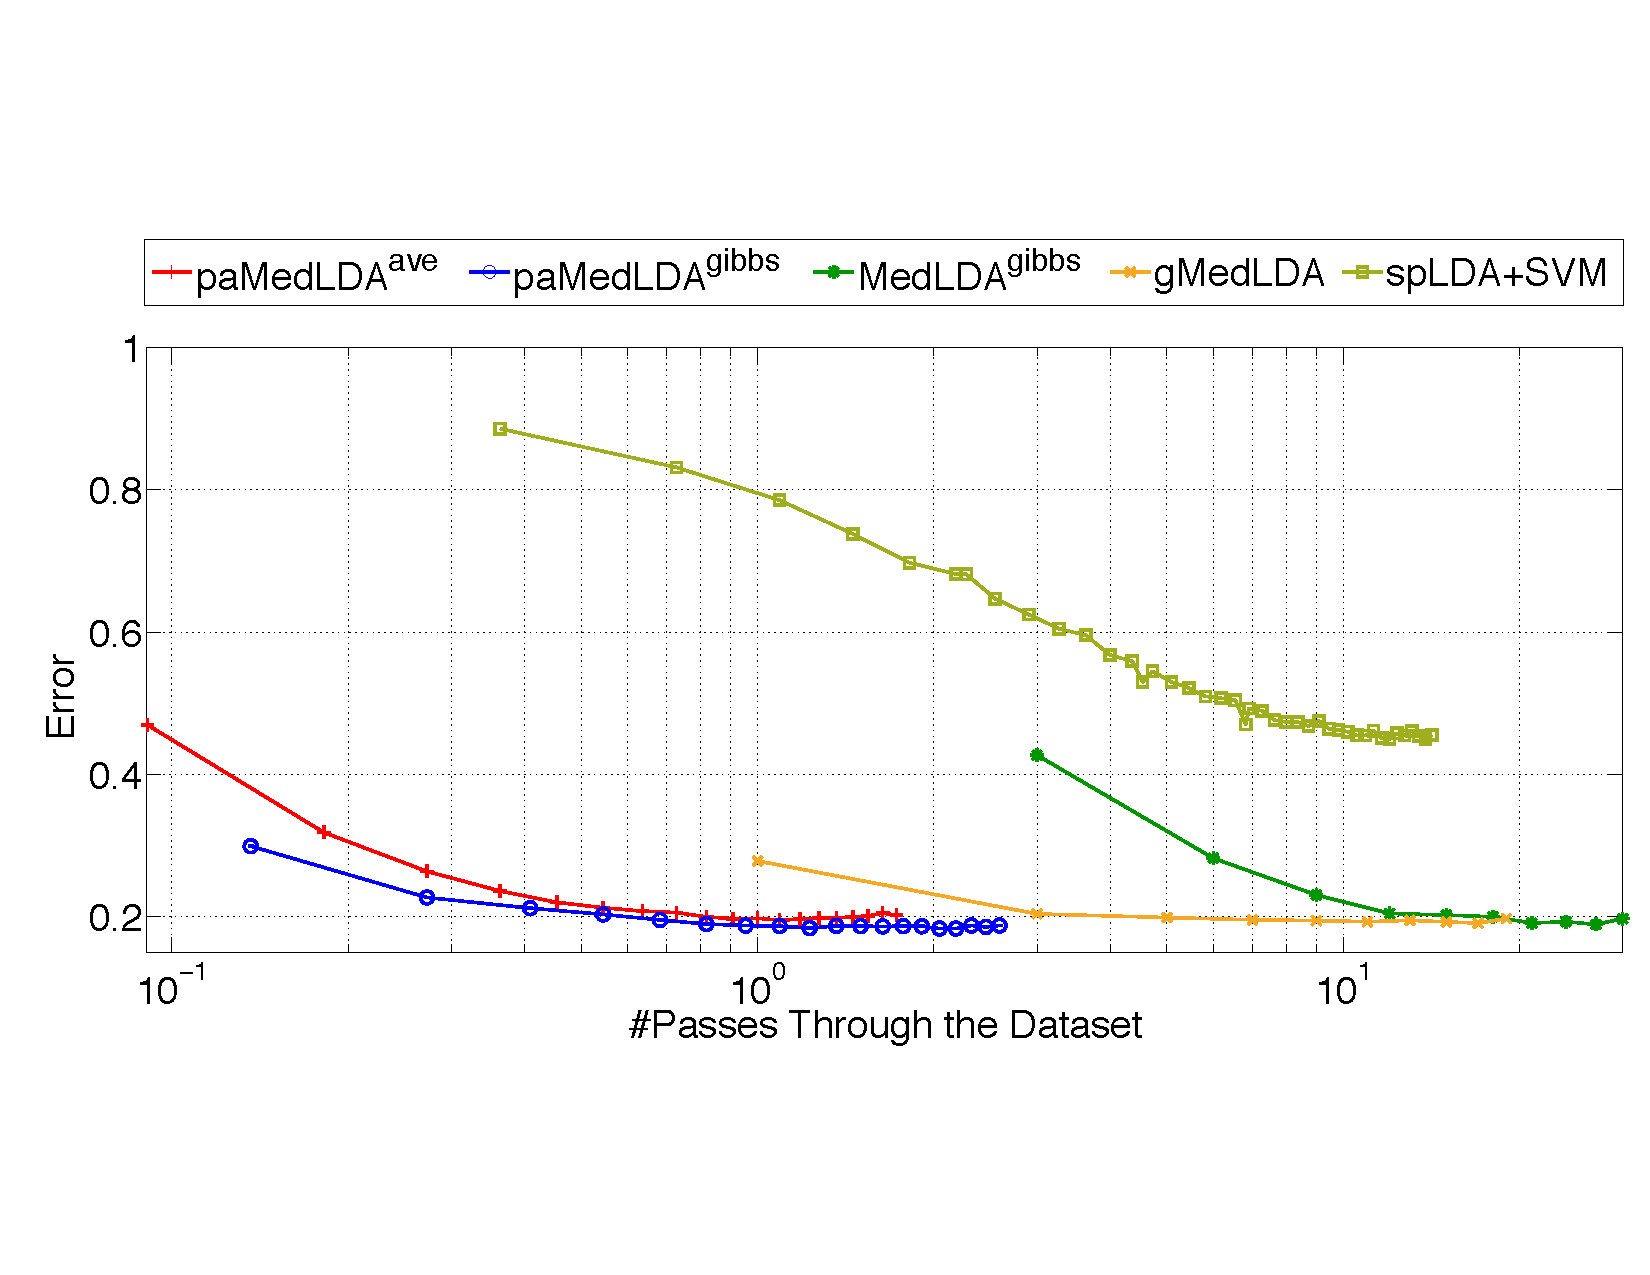
\includegraphics[width = .9\textwidth]{plot_multic_commit_lda_jmlr.pdf}
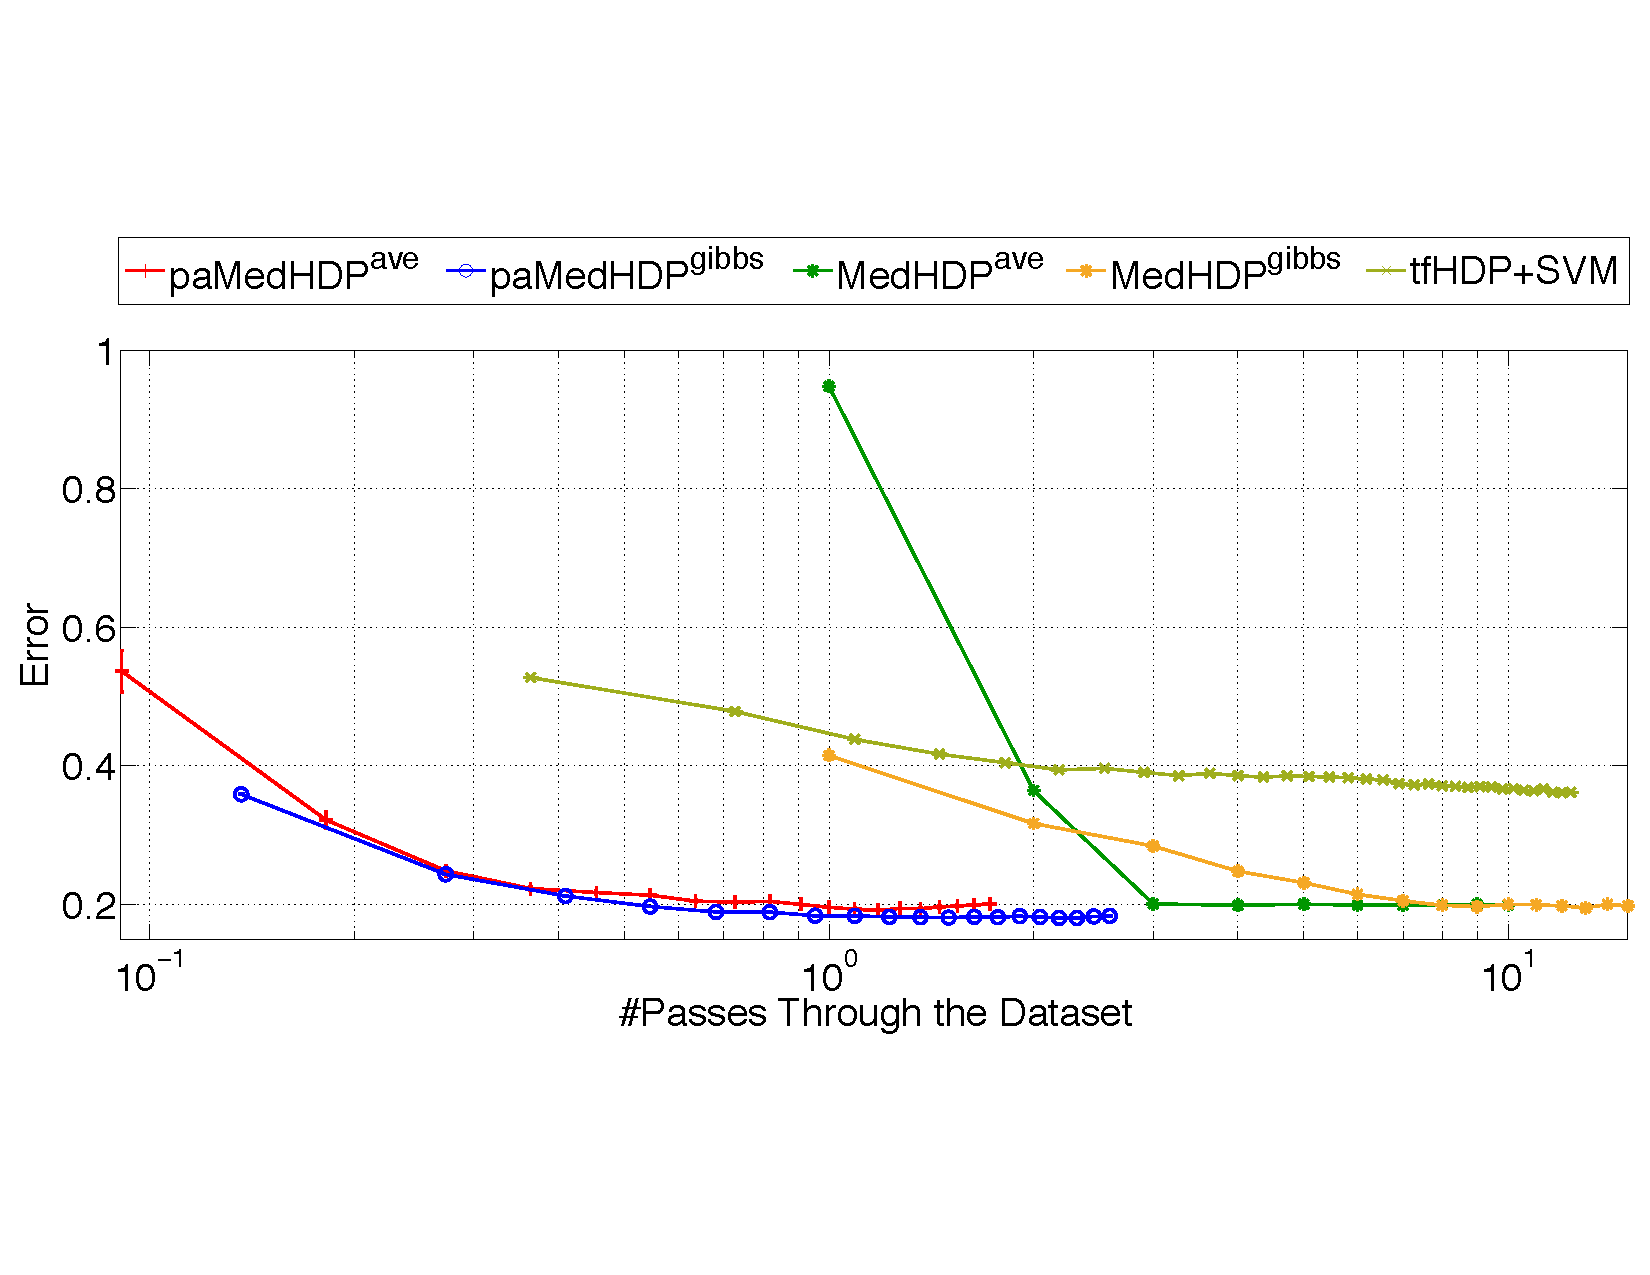
\includegraphics[width = 0.89\textwidth]{plot_multic_commit_hdp_jmlr.pdf}
\end{center}\vspace*{-0.2cm}
\caption{Test errors of different models with respect to the number of passes through the 20NG training data set. }
\vspace*{-0.2cm}
\label{fg:multic_commit}
\end{figure}





We use shorthand notations \paMedLDAave and \paMedLDAgibbs for online MedLDA and online Gibbs MedLDA respectively. The batch counterparts are MedLDA~\citep{zhu2012medlda} and Gibbs MedLDA (\MedLDAgibbs)~\citep{zhugibbs2013}, which is a MedLDA model with Gibbs classifiers. We use collapsed Gibbs sampling to solve MedLDA, which is exactly the gMedLDA model proposed by~\cite{jiang2012monte}. We also choose a state-of-the-art online unsupervised topic model as the baseline, the sparse inference for LDA (spLDA) \citep{mimno2012sparse}, which has been demonstrated to be superior than the stochastic variational LDA \citep{hoffman2013stochastic} in prediction performance. To perform the supervised tasks, we learn a linear SVM with the topic representations using LIBSVM \citep{chang2011libsvm}. We refer the readers to~\citep{zhu2012medlda} for the performances of other batch-learning-based supervised topic models, such as sLDA \citep{blei2010supervised} and DiscLDA \citep{lacoste2008disclda}, as well as SVM classifiers on the raw inputs, which are generally either inferior in accuracy or slower in efficiency than MedLDA. For all the LDA-based topic models, we use symmetric Dirichlet priors $\bm{\alpha} = 1/K \cdot \bm{1}$ and $\bm{\gamma} = 0.45 \cdot \bm{1}$. For BayesPA with Gibbs classifiers, the parameters were set at $\epsilon = 164$, $c = 1$, and $\sigma^2 = 1$. The models' performance is not sensitive to the choice of these parameters in wide ranges as shown in \cite{zhugibbs2013}. For BayesPA with averaging classifiers, the parameters determined by cross validation are $\epsilon = 16$, $c = 500$, and $\sigma^2 = 10^{-3}$. For reasons explained in section \ref{sec:sensitivity}, we set the mini-batch size $|B| = 1$ for the averaging classifier and $|B| = 512$ for the Gibbs classifier.

We first analyze how many processed documents are sufficient for each model to converge. Figure \ref{fg:multic_commit} shows the test errors with respect to the number of passes through the 20NG training set, where the number of topics is set at $K = 80$ and the other parameters of BayesPA are set at $(\mathcal{I}, \mathcal{J}, \beta) = (1, 2, 0)$. As we can observe, by solving a series of latent BayesPA problems, both \paMedLDAave and \paMedLDAgibbs fully explore the redundancy of documents and converge in  less than one pass, while their batch counterparts (i.e., MedLDA and \MedLDAgibbs) need many passes as burn-in steps. Besides, compared with the online learning algorithms for unsupervised topic models (i.e., spLDA+SVM), BayesPA topic models use supervising side information from each mini-batch, and therefore exhibit a faster convergence rate in discrimination ability. The convergence performance of BayesPA models is significantly better than that of the unsupervised spLDA.
% By solving a series of latent Passive-Aggressive learning problems with hybrid variational inference and data augmentation trick, paMedLDA converges to its batch alternatives in a single pass.
%Besides, among the batch algorithms, bMedLDA  requires fewer passes than gMedLDA, probably because it uses multiple local samples for each global update, thus being more stable.


Next, we study each model's best performance possible and the corresponding training time.
%For test time, paMedLDA adopts the same testing approach as Gibbs MedLDA,  \citep{zhugibbs2013} provides a detailed comparison of test time.
To allow for a fair comparison, we train each model until the relative change of  its objective is less than $10^{-4}$.
%$\mathcal{M} = 8$ for bMedLDA, $\mathcal{M} = 30$ for gMedLDA, and number of passes $\mathcal{E} = 3$ for oLDA, $\mathcal{E} = 10$ for tfHDP.
%In particular, we use a single pass for paMedLDA.
 Figure \ref{fg:multic_topic_lda} shows the prediction accuracy and training time of LDA-based models on the whole data set with varying numbers of topics. We can see that BayesPA topic models are more than an order of magnitude faster than their batch counterparts in training time due to the power of online learning. \paMedLDAave is faster than \paMedLDAgibbs, because it does not need to update the covariance matrix of classifier weights $\wv$. But the tradeoff is that for averaging models, they are more sensitive to the initial choice of $\sigma^2$, and therefore we need to use cross-validation to determine the best choice of variance beforehand.
 % however, paMedLDAave is more sensitive to the choice of initial weight variance.
Furthermore, thanks to the merits of structured mean-field inference, which does not impose strict assumptions on the independence of latent variables, BayesPA topic models parallel their batch alternatives in accuracy. Moreover, all the supervised models are significantly better than the unsupervised spLDA in classification, reaching the state-of-the-art performance on the tested datasets.
\begin{figure}[t]
\centering
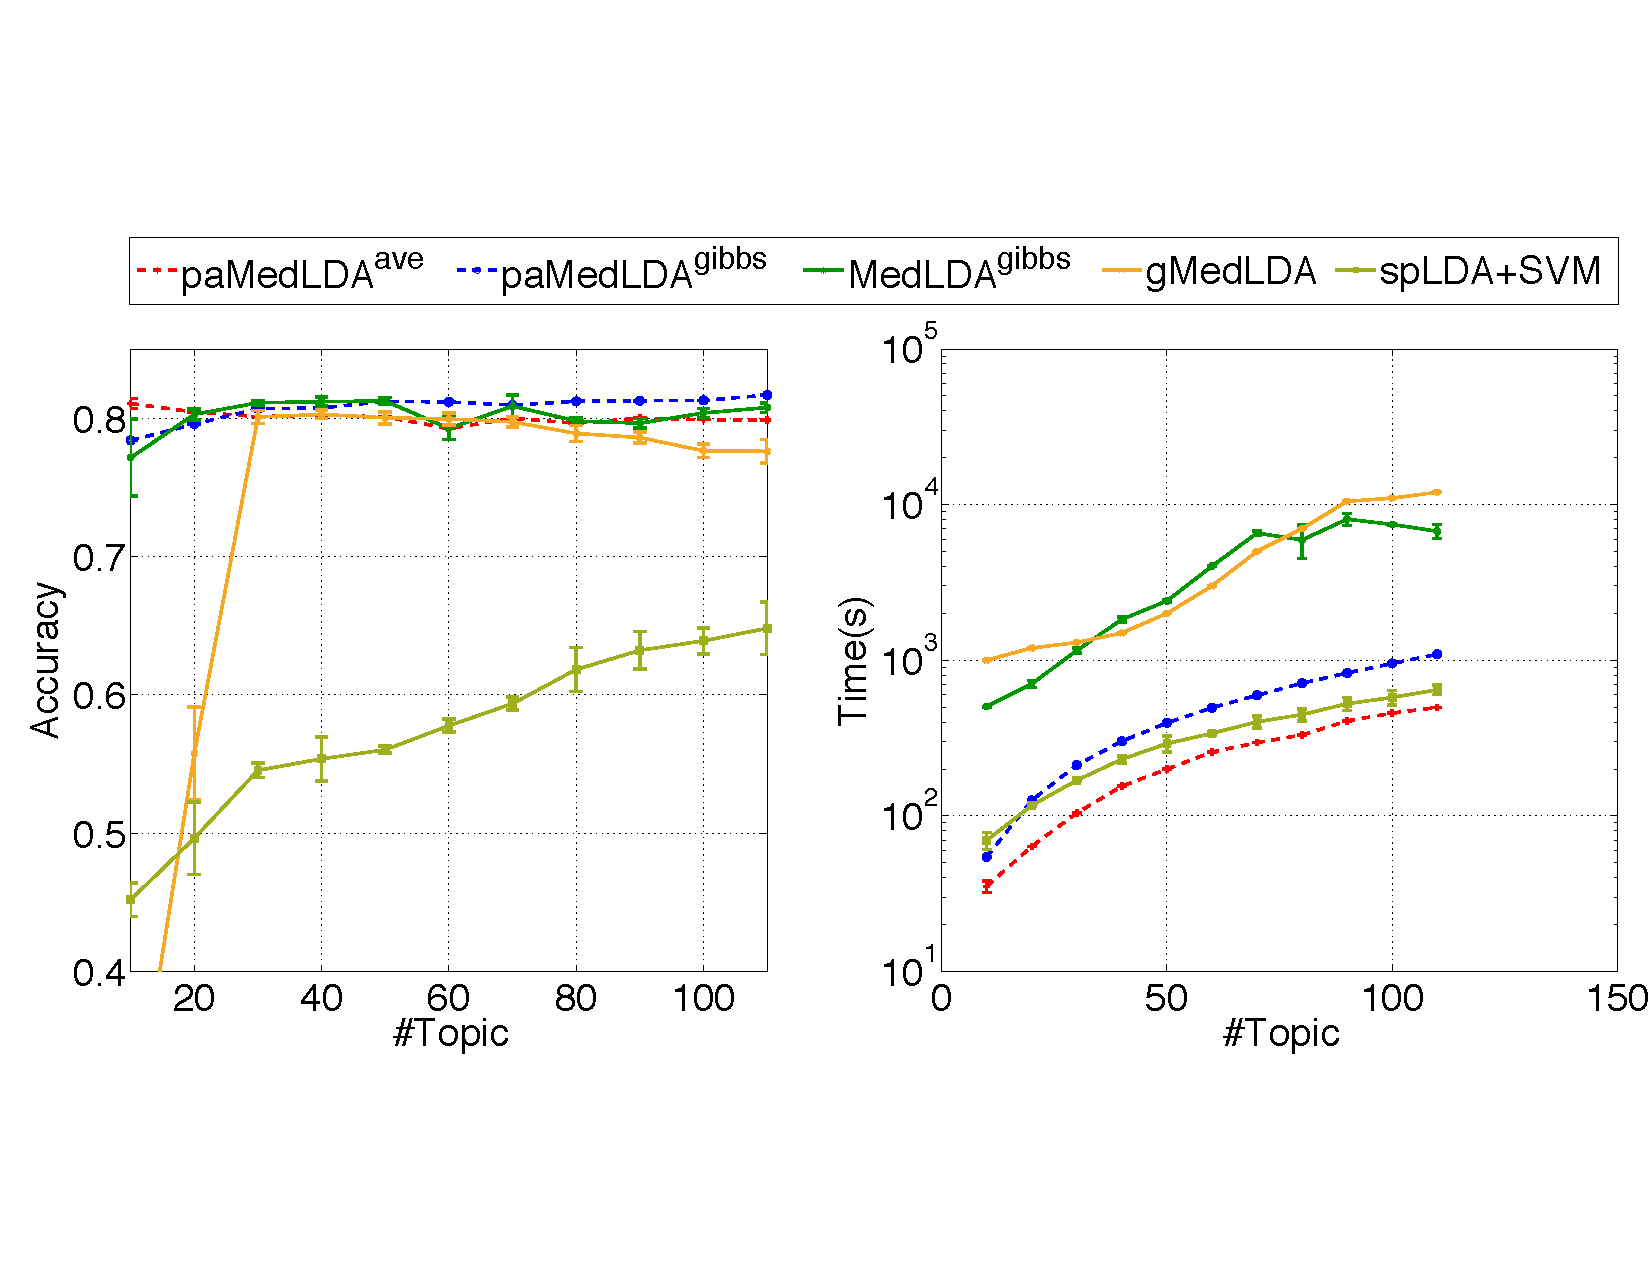
\includegraphics[width = .95\textwidth]{plot_acc_topic_multic_lda.pdf}
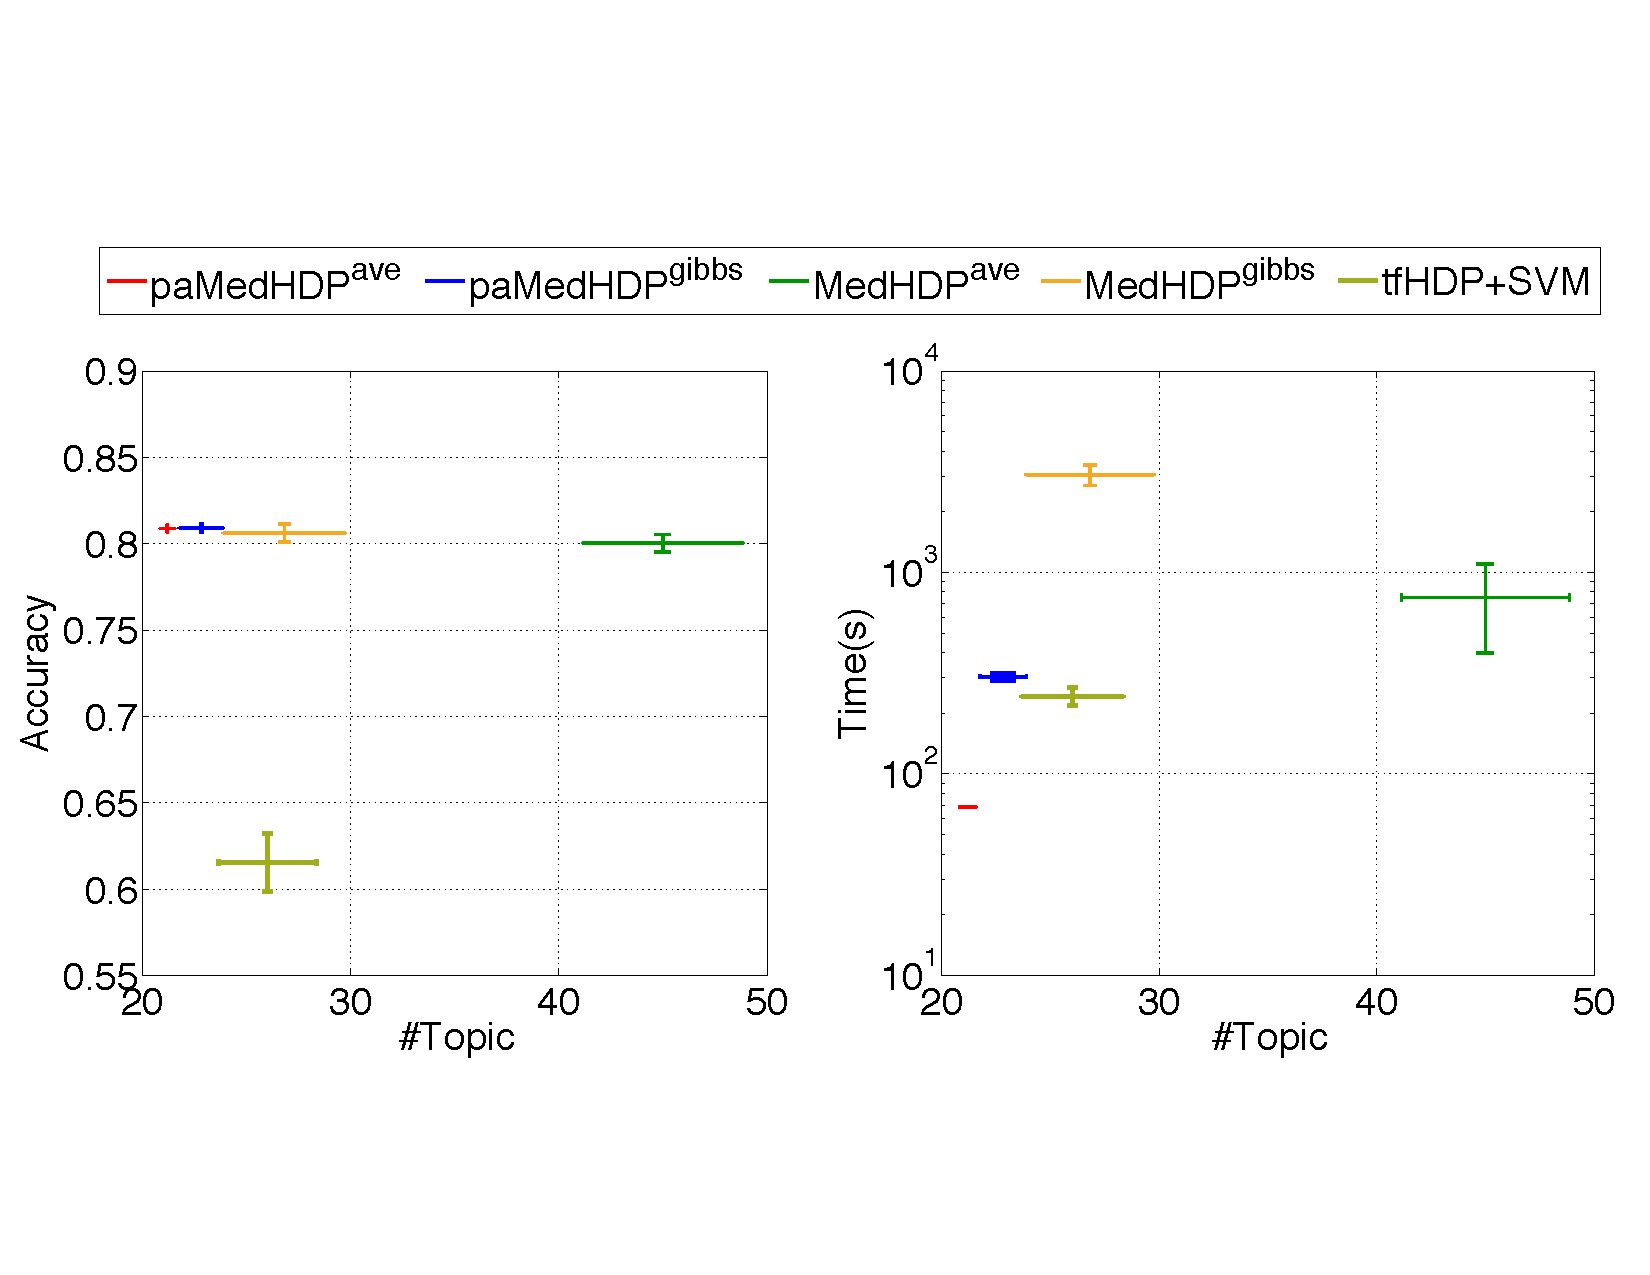
\includegraphics[width = .95\textwidth]{plot_acc_topic_multic_hdp.pdf}\vspace*{-.2cm}
\caption{Classification accuracy and running time of various models with respect to the number of topics on the 20NG data set.}\vspace*{-0.3cm}
\label{fg:multic_topic_lda}
\end{figure}
%\begin{figure}[t]
%\caption{Classification accuracy and running time of the nonparametric paMedHDP and its batch counterpart models on the 20NG data set.
%\strin{Batch MedHDP is obtained by setting $|B| = D$ in online BayesPA. Is this a *fair* batch counterpart? This method uses Chong Wang's truncation-free method for nonparametric inference, which is kind of awkward. Should we compare with MedHDP implemented otherwise, say split and merge?}
%}
%\label{fg:multic_topic_hdp}
%\end{figure}





%\newpage
\begin{table}[t]
\newcommand\barw{0.1}
\begin{center}
\scalebox{0.95}
{ \begin{tabular}{|c|r|c|}
\hline\hline
\multicolumn{3}{|c|}{{\bf Results by \paMedLDAave}}  \\
\hline
Category & \multicolumn{2}{|c|}{Visualization}  \\
\hline

\multirow{6}{*}{alt.altheism} &
\#Observation &
\begin{tabularx}{0.6\textwidth}{XXXXX}
 1 & 64 & 512 & 4096 & 11269 \\
\end{tabularx} \\

& Topic distribution &
\begin{tabular}{ccccc}
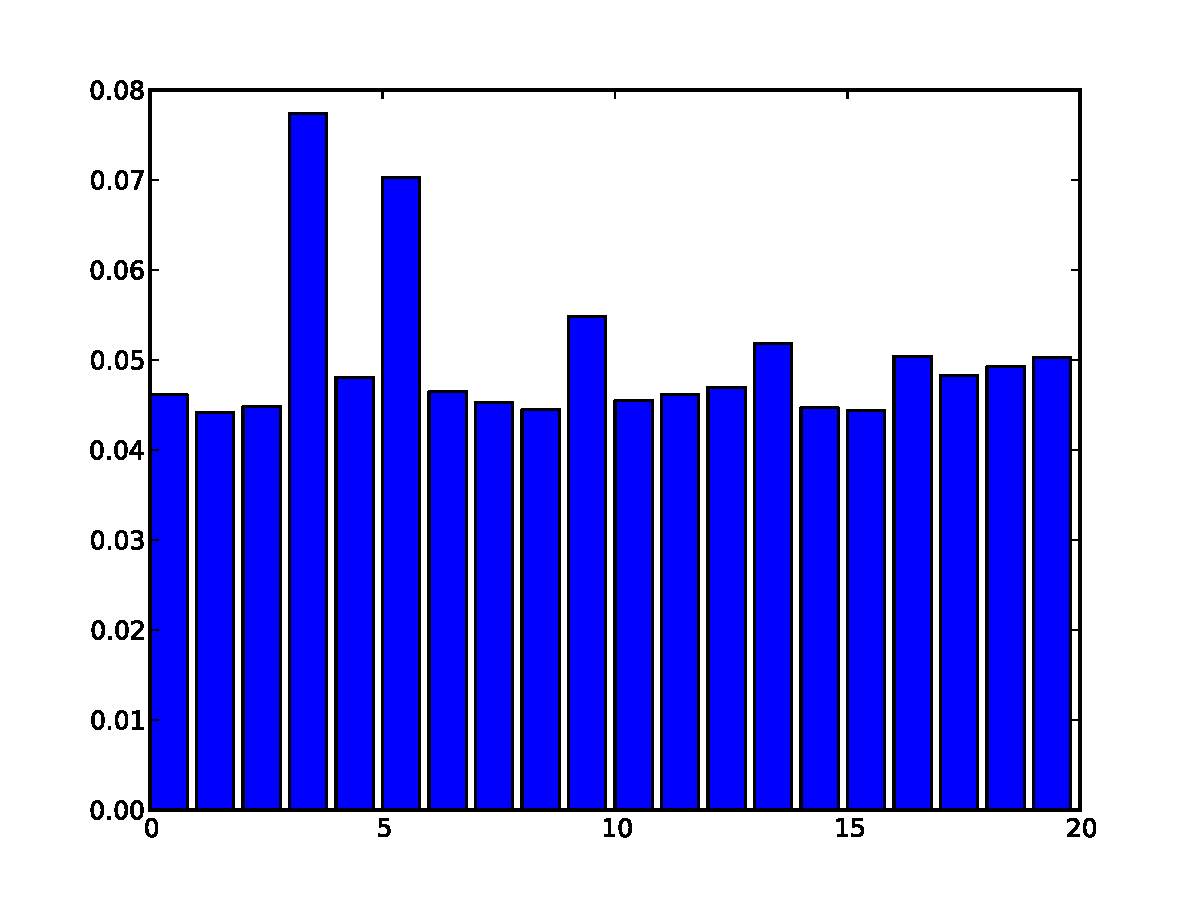
\includegraphics[width=\barw\textwidth]{visualize_dist_paMedLDAave_0/0_1} &
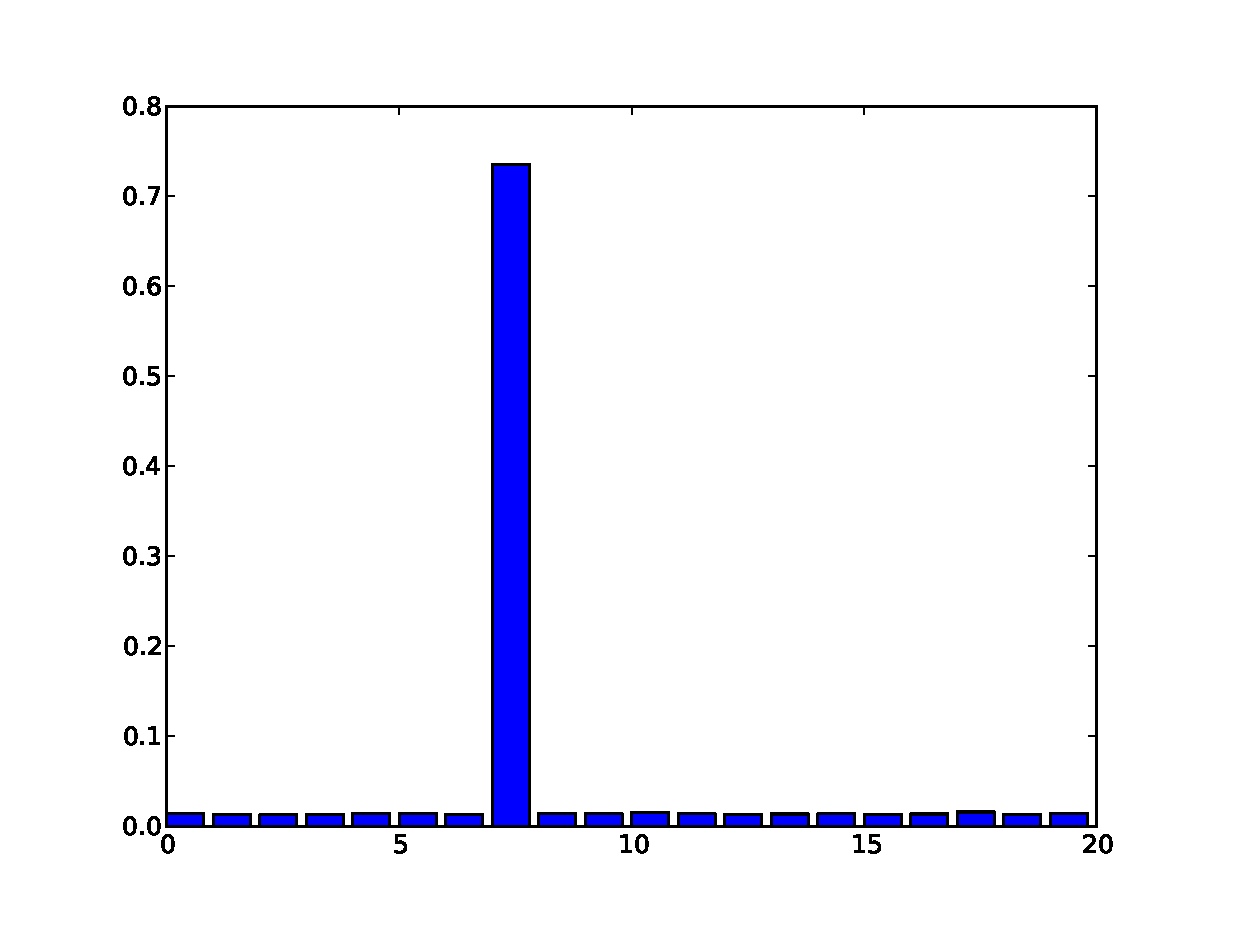
\includegraphics[width=\barw\textwidth]{visualize_dist_paMedLDAave_0/0_64}
&
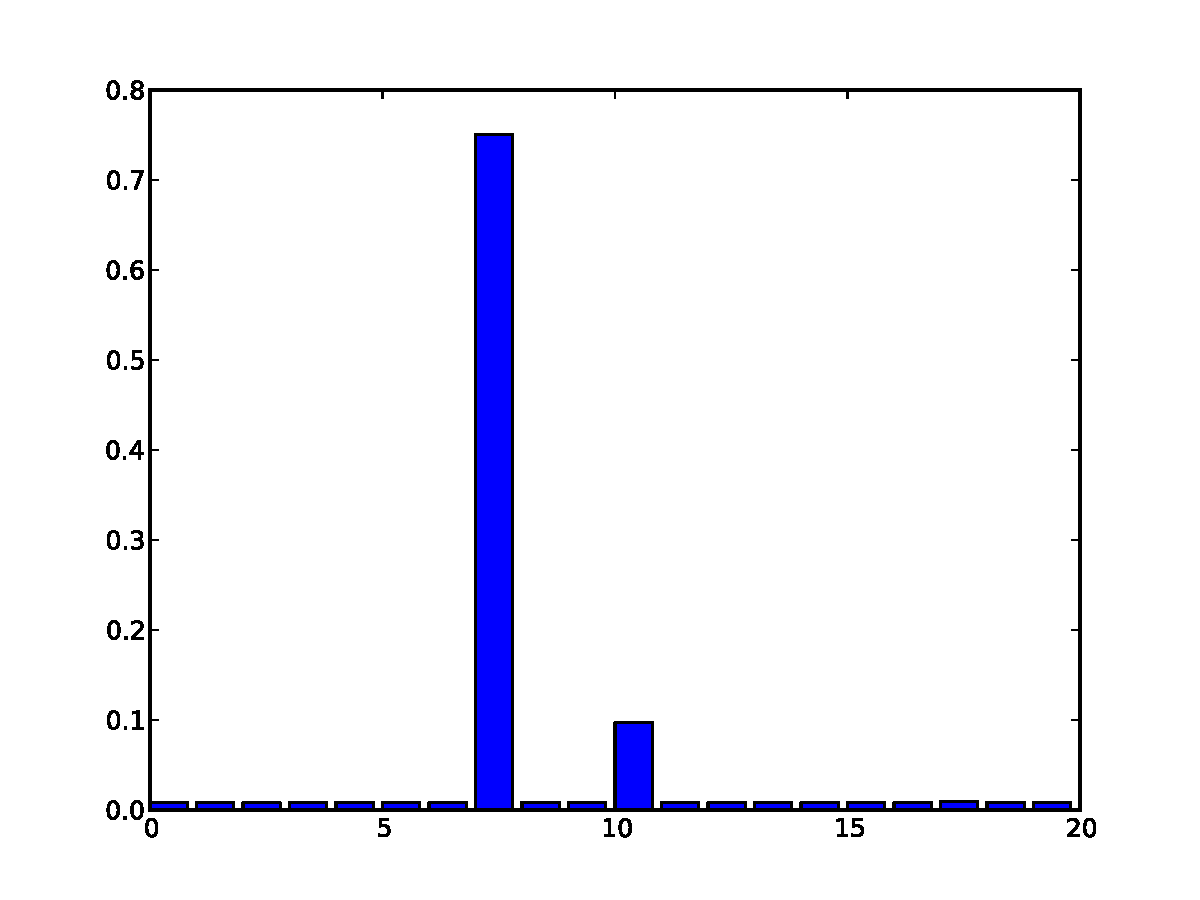
\includegraphics[width=\barw\textwidth]{visualize_dist_paMedLDAave_0/0_512} &
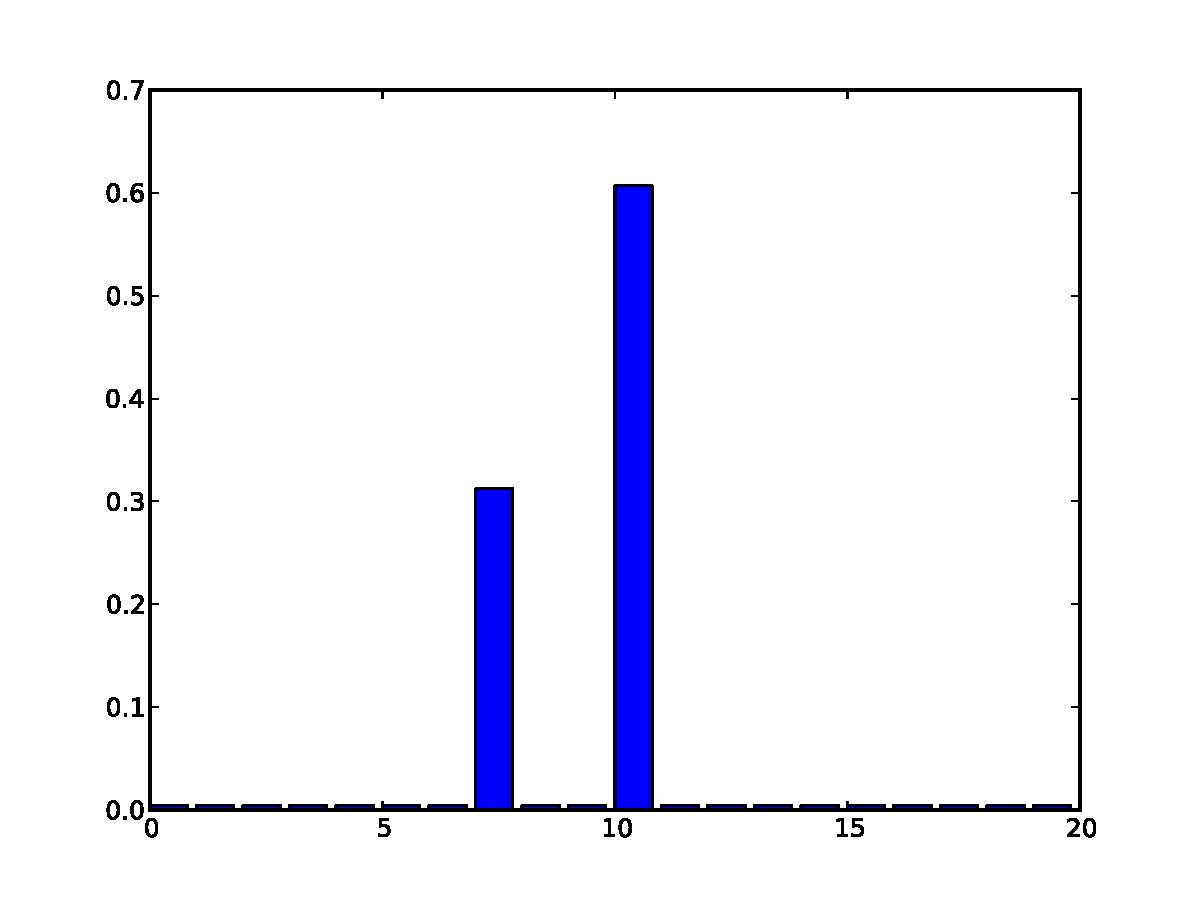
\includegraphics[width=\barw\textwidth]{visualize_dist_paMedLDAave_0/0_4096} &
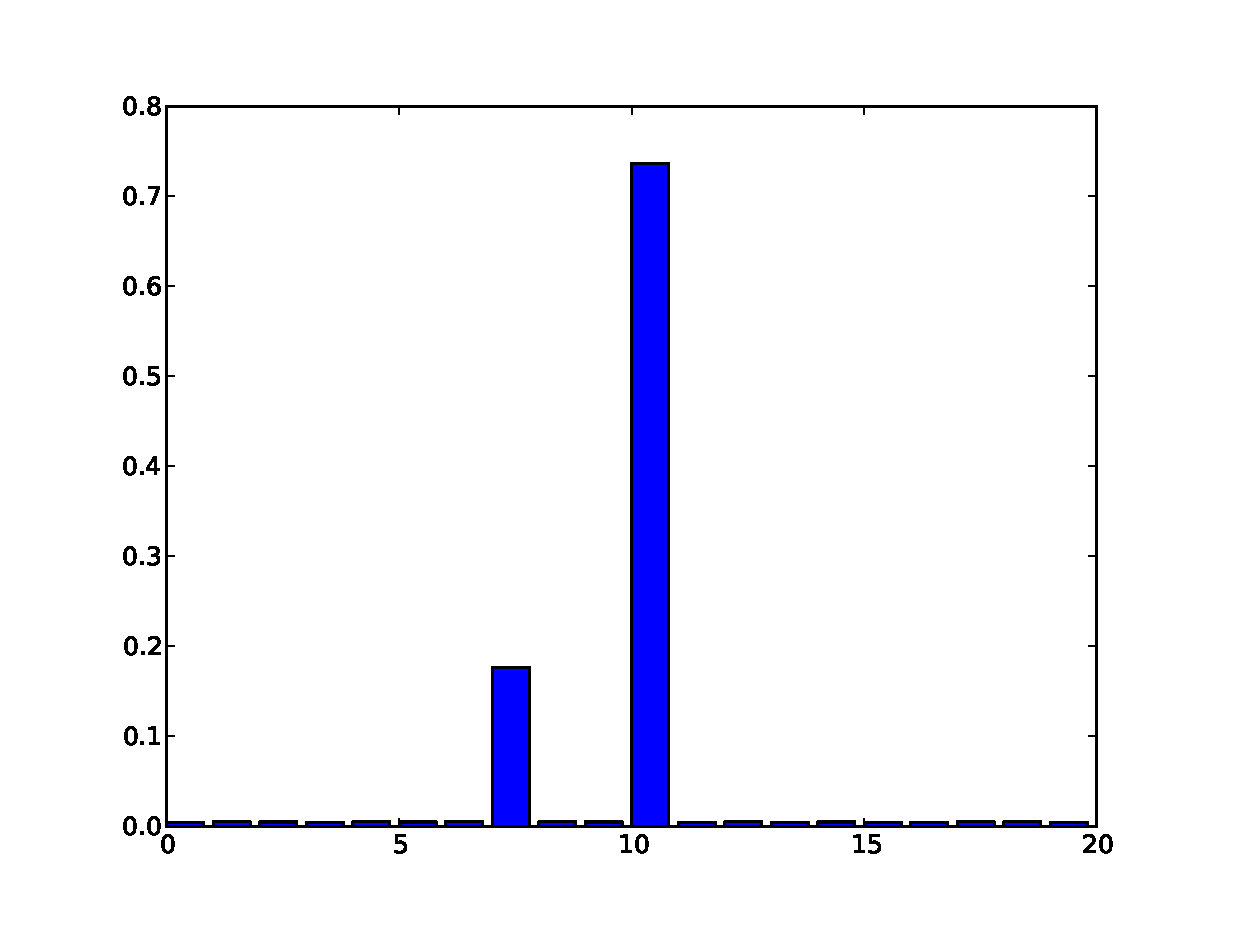
\includegraphics[width=\barw\textwidth]{visualize_dist_paMedLDAave_0/0_11269} \\
\hline
\end{tabular} \\

& Top words &
\begin{tabular}{r|cccccc}
 T8 & writes & article & don & people & time & good \\
 T11 & god & people & writes & don & article & atheism
\end{tabular}
\\


\hline

\multirow{6}{*}{comp.graphics} &
\#Observation &
\begin{tabularx}{0.6\textwidth}{XXXXX}
 1 & 64 & 512 & 4096 & 11269 \\
\end{tabularx} \\

& Topic distribution &
\begin{tabular}{ccccc}
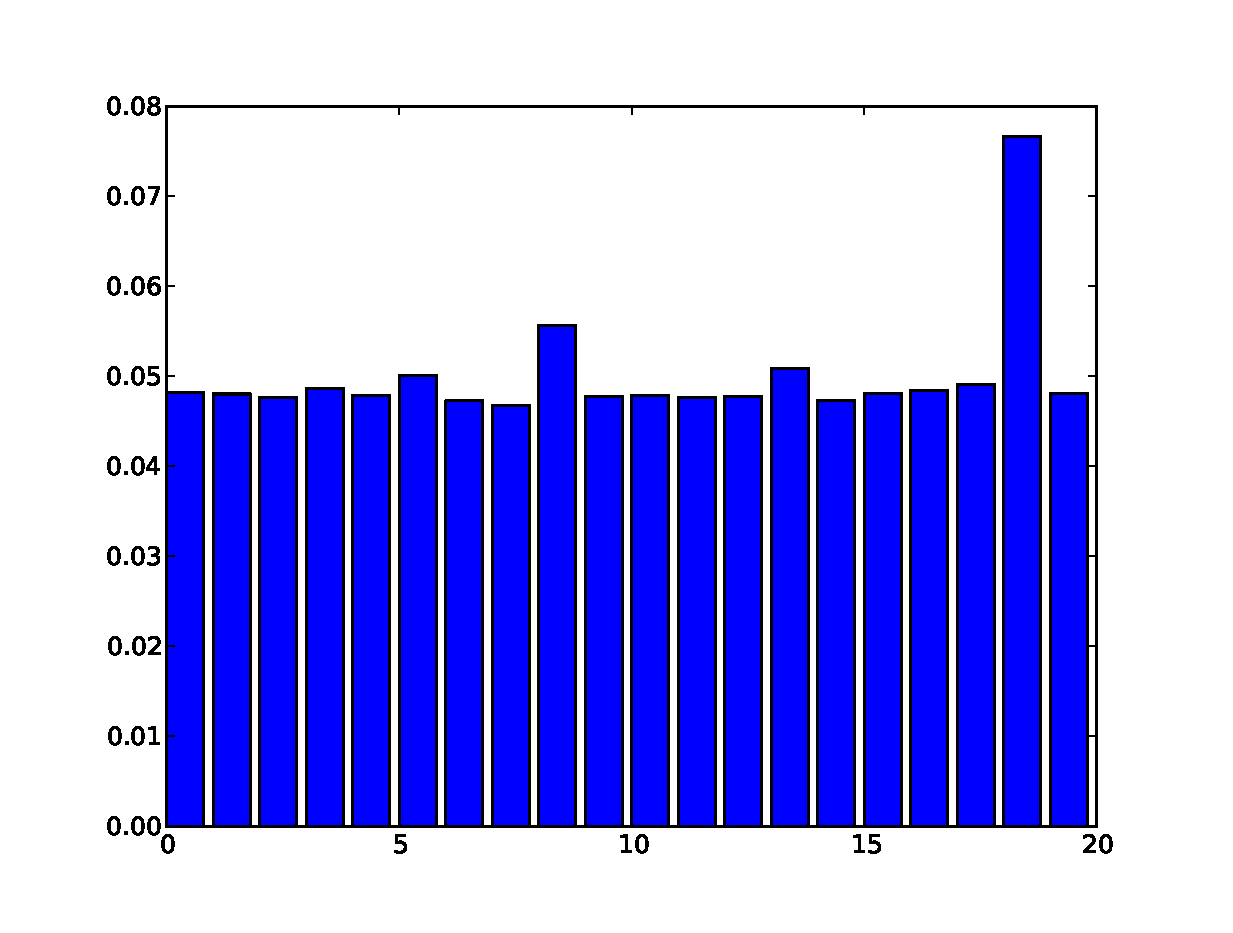
\includegraphics[width=\barw\textwidth]{visualize_dist_paMedLDAave_1/1_1} &
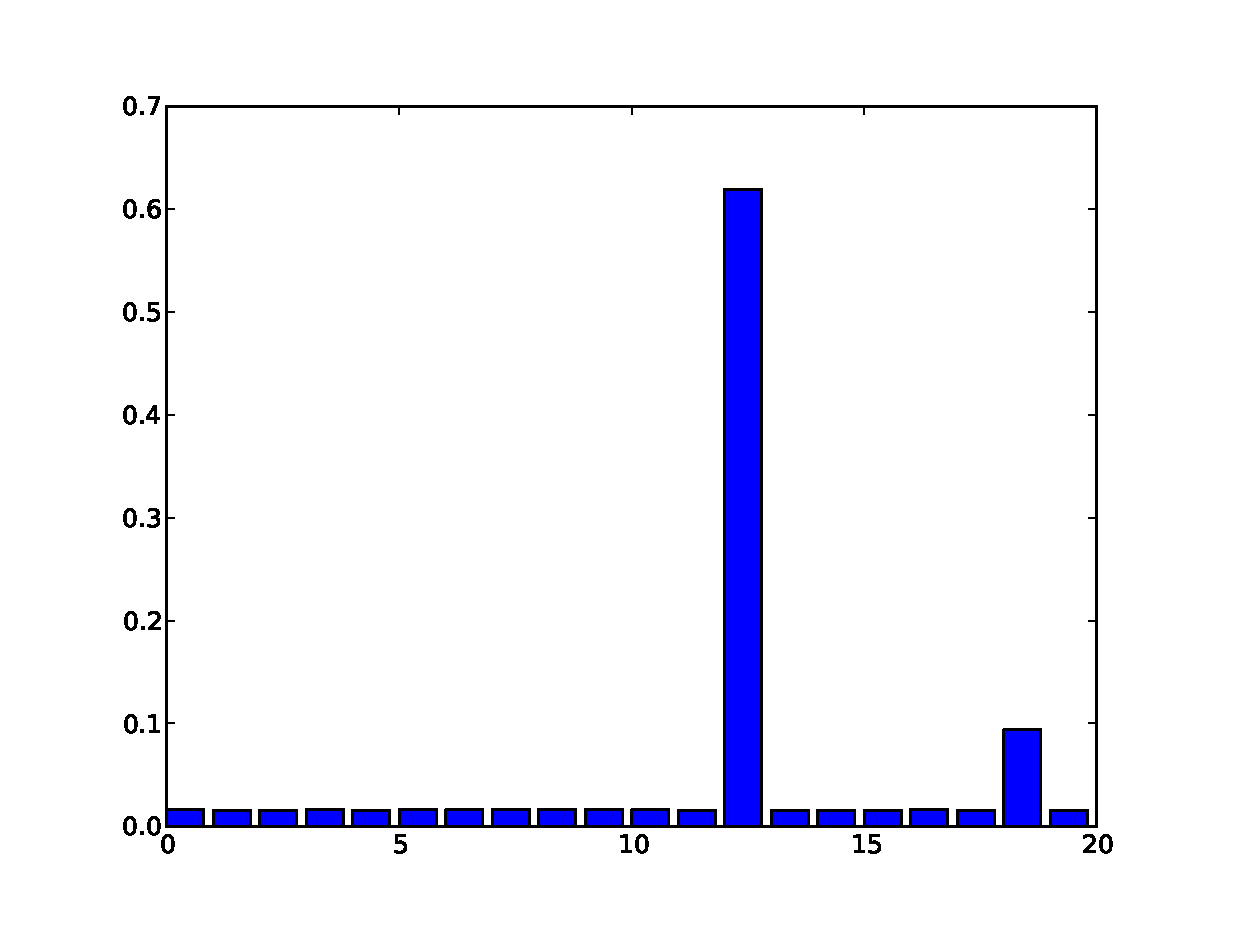
\includegraphics[width=\barw\textwidth]{visualize_dist_paMedLDAave_1/1_64}
&
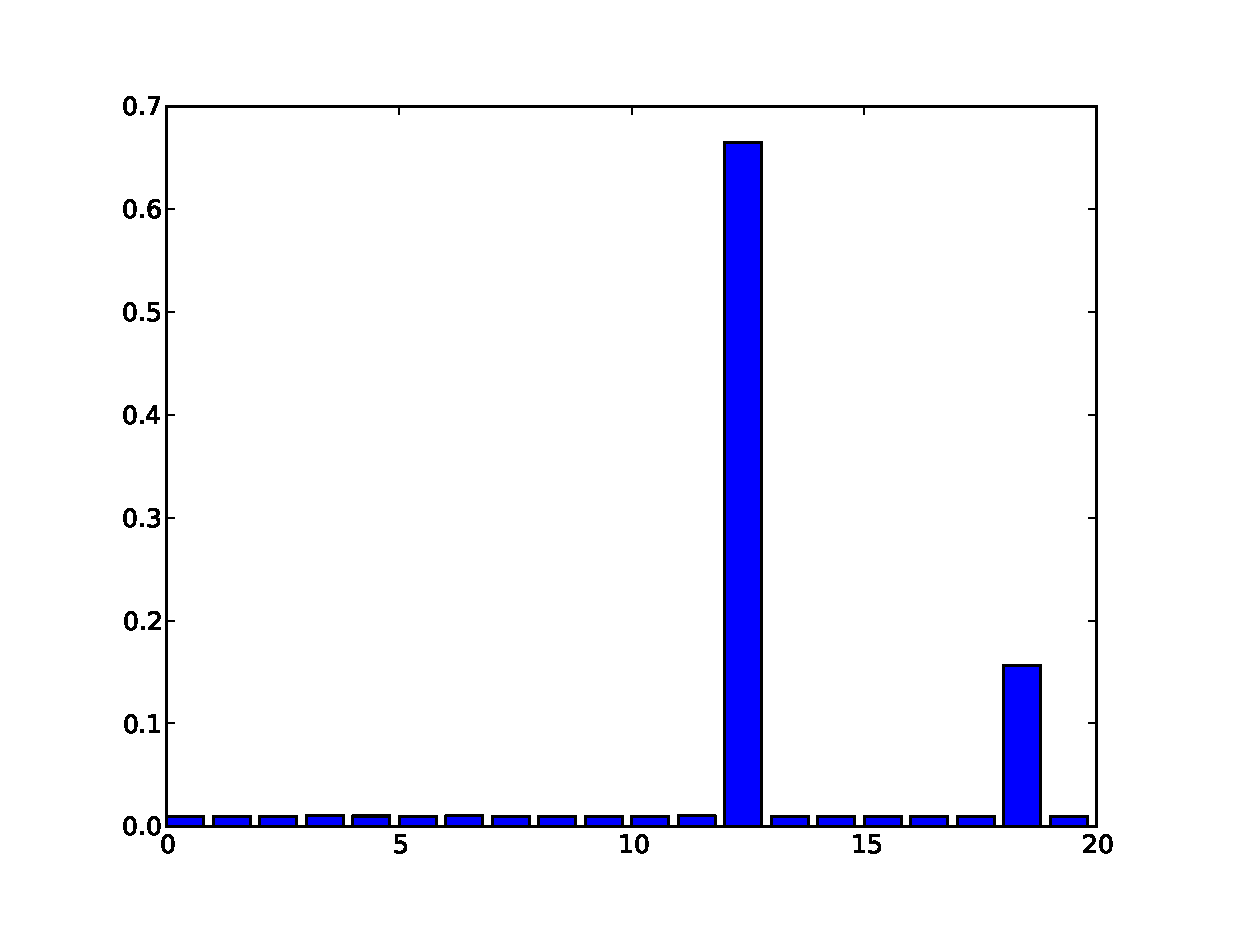
\includegraphics[width=\barw\textwidth]{visualize_dist_paMedLDAave_1/1_512} &
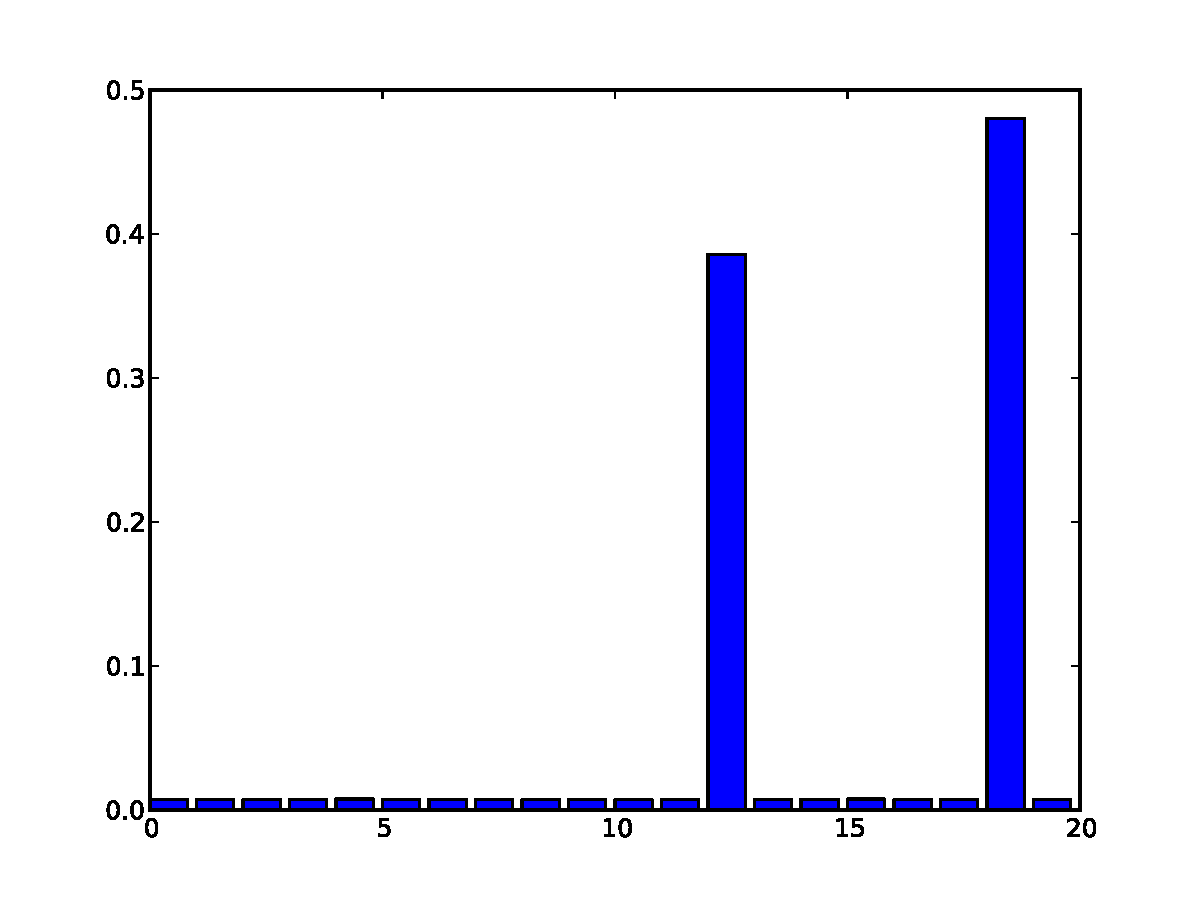
\includegraphics[width=\barw\textwidth]{visualize_dist_paMedLDAave_1/1_4096} &
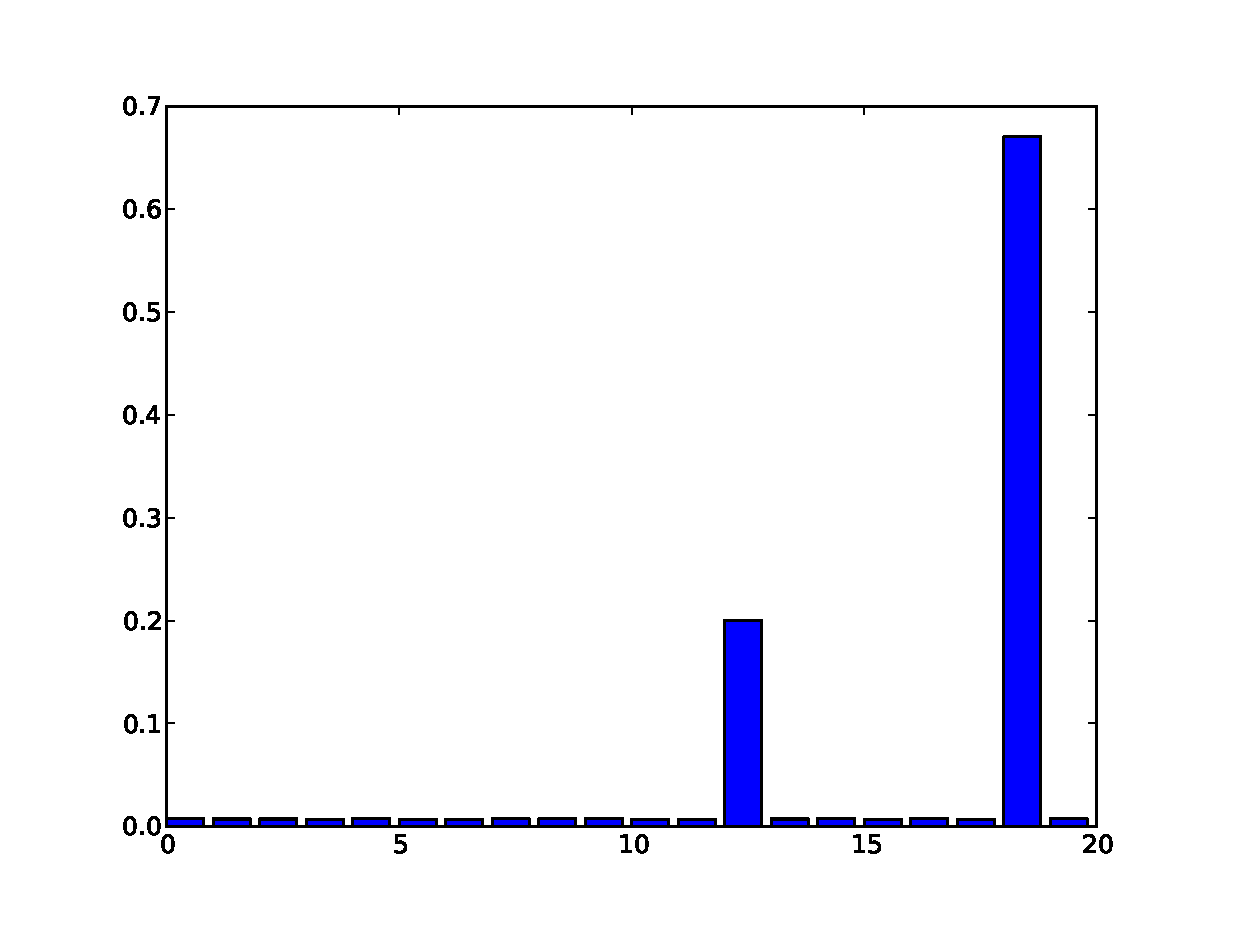
\includegraphics[width=\barw\textwidth]{visualize_dist_paMedLDAave_1/1_11269} \\
\hline
\end{tabular} \\

& Top words &
\begin{tabular}{r|cccccc}
 T19 & image & graphics & file & jpeg & files & software \\
 T13 & writes & article & people & don & time & good
\end{tabular}
\\

\hline

\multirow{6}{*}{misc.forsale} &
\#Observation &
\begin{tabularx}{0.6\textwidth}{XXXXX}
 1 & 64 & 512 & 4096 & 11269 \\
\end{tabularx} \\

& Topic distribution &
\begin{tabular}{ccccc}
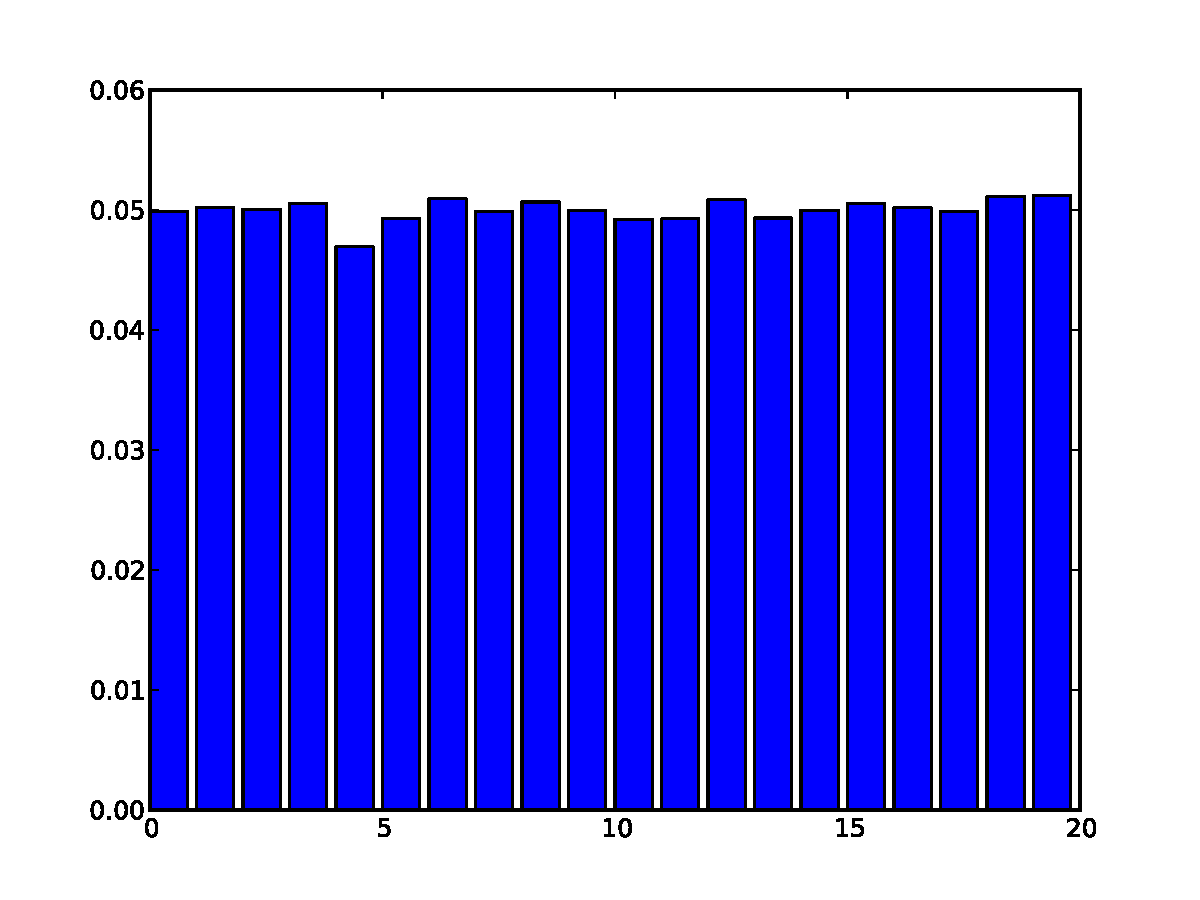
\includegraphics[width=\barw\textwidth]{visualize_dist_paMedLDAave_6/6_1} &
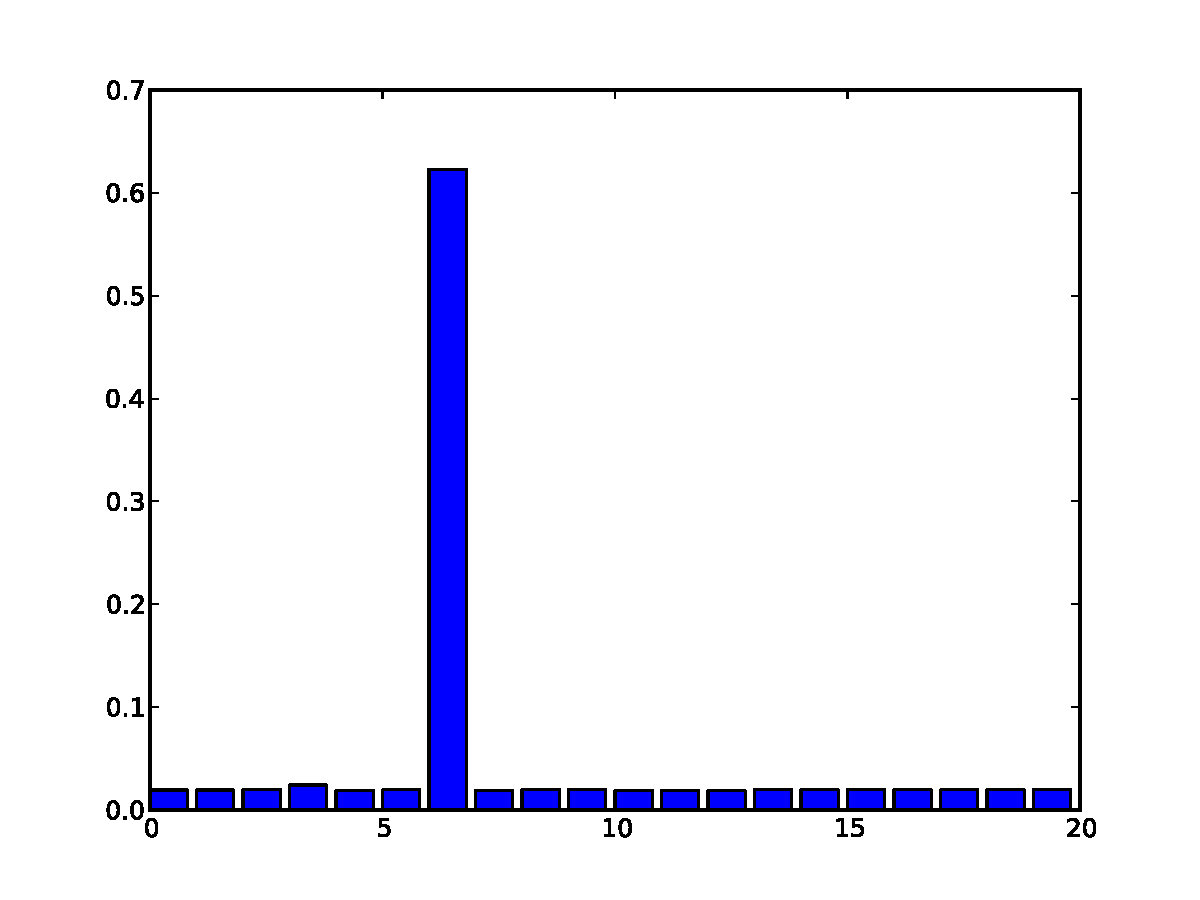
\includegraphics[width=\barw\textwidth]{visualize_dist_paMedLDAave_6/6_64}
&
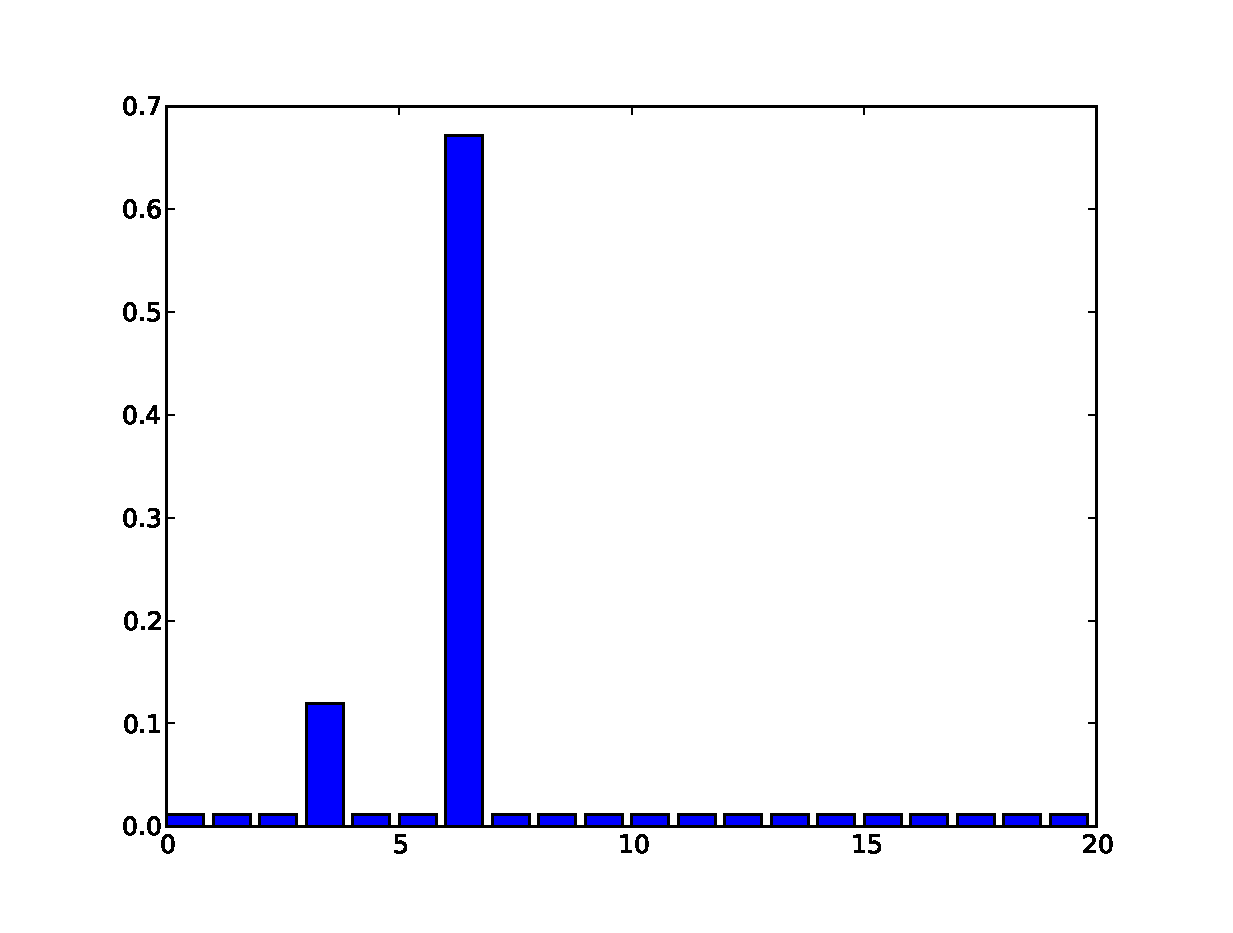
\includegraphics[width=\barw\textwidth]{visualize_dist_paMedLDAave_6/6_512} &
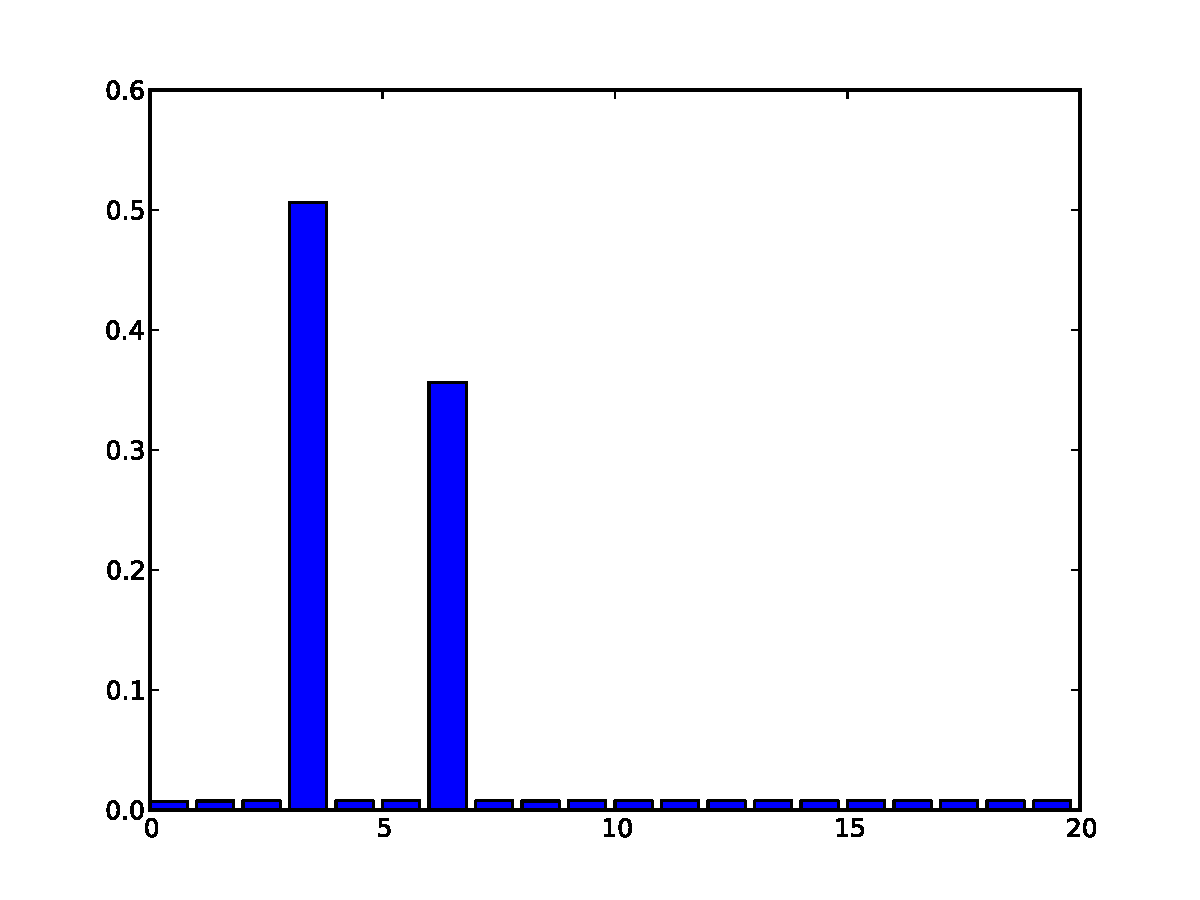
\includegraphics[width=\barw\textwidth]{visualize_dist_paMedLDAave_6/6_4096} &
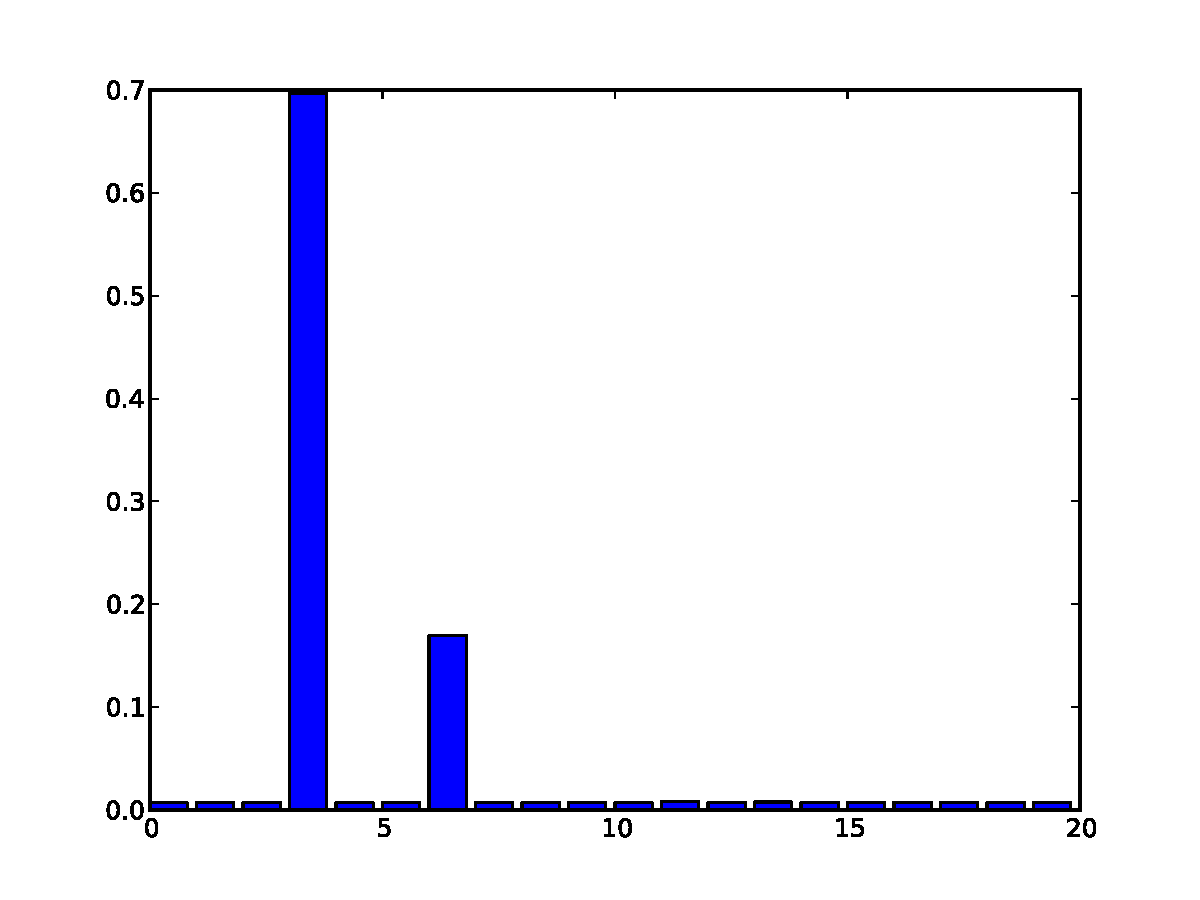
\includegraphics[width=\barw\textwidth]{visualize_dist_paMedLDAave_6/6_11269} \\
\hline
\end{tabular} \\

& Top words &
\begin{tabular}{r|cccccc}
 T4 & sale & offer & shipping & mail & dos & price \\
 T8 & writes & article & people & don & time & good
\end{tabular}
\\


\hline\hline
%\end{tabular}
%\end{center}
%\caption{Visualization of Learnt Topics by \paMedLDAave}
%\label{tb:visualization_ave}
%\end{table}
%
%
%\begin{table}[t]
%\newcommand\barw{0.1}
%\begin{center}
%\begin{tabular}{|c|r|c|}
\multicolumn{3}{|c|}{{\bf Results by \paMedLDAgibbs}}  \\
\hline
Category & \multicolumn{2}{|c|}{Visualization}  \\
\hline


\multirow{6}{*}{alt.altheism} &
\#Observation &
\begin{tabularx}{0.6\textwidth}{XXXXX}
 1 & 64 & 512 & 4096 & 11269 \\
\end{tabularx} \\

& Topic distribution &
\begin{tabular}{ccccc}
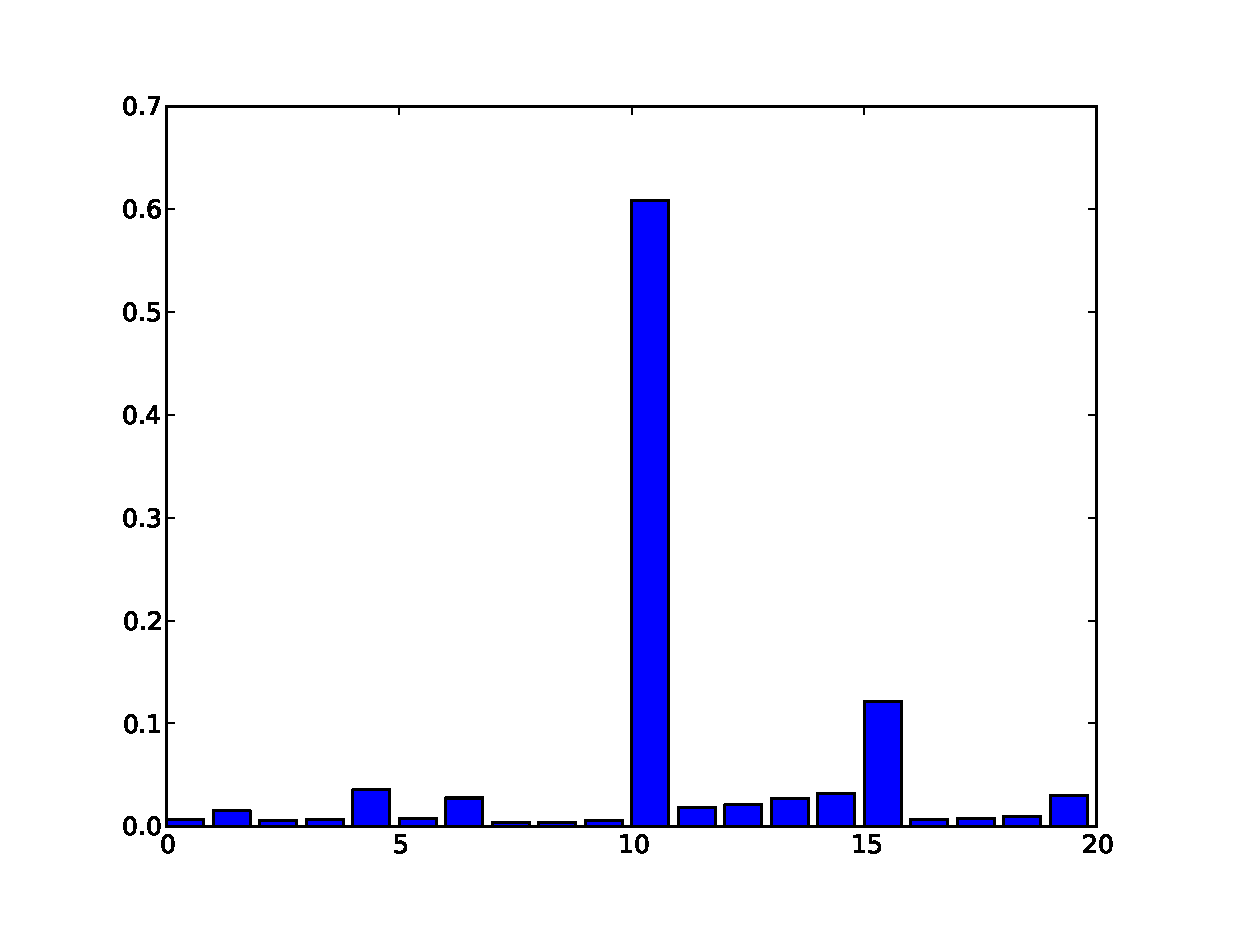
\includegraphics[width=\barw\textwidth]{visualize_dist_paMedLDAgibbs_0/0_0} &
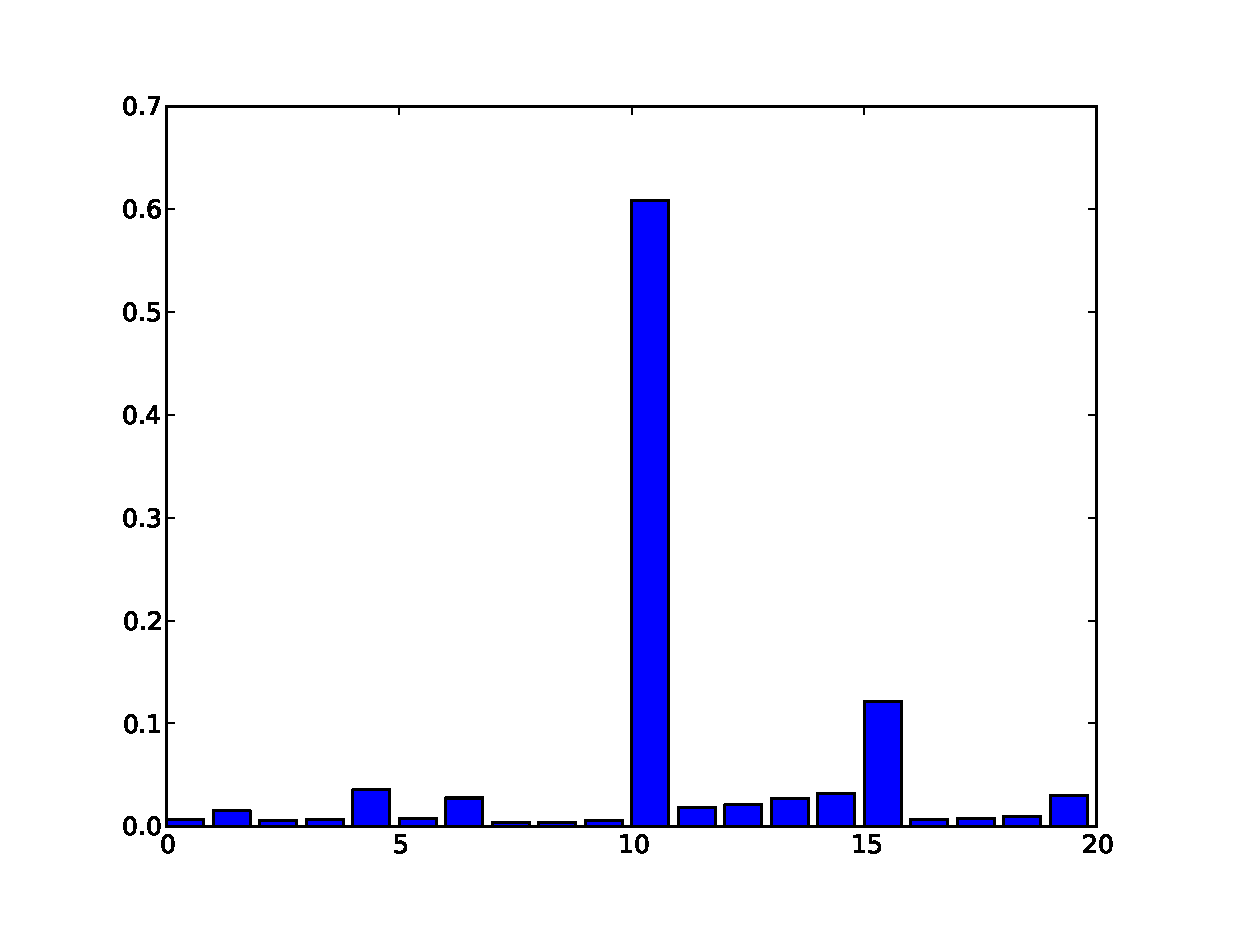
\includegraphics[width=\barw\textwidth]{visualize_dist_paMedLDAgibbs_0/0_0}
&
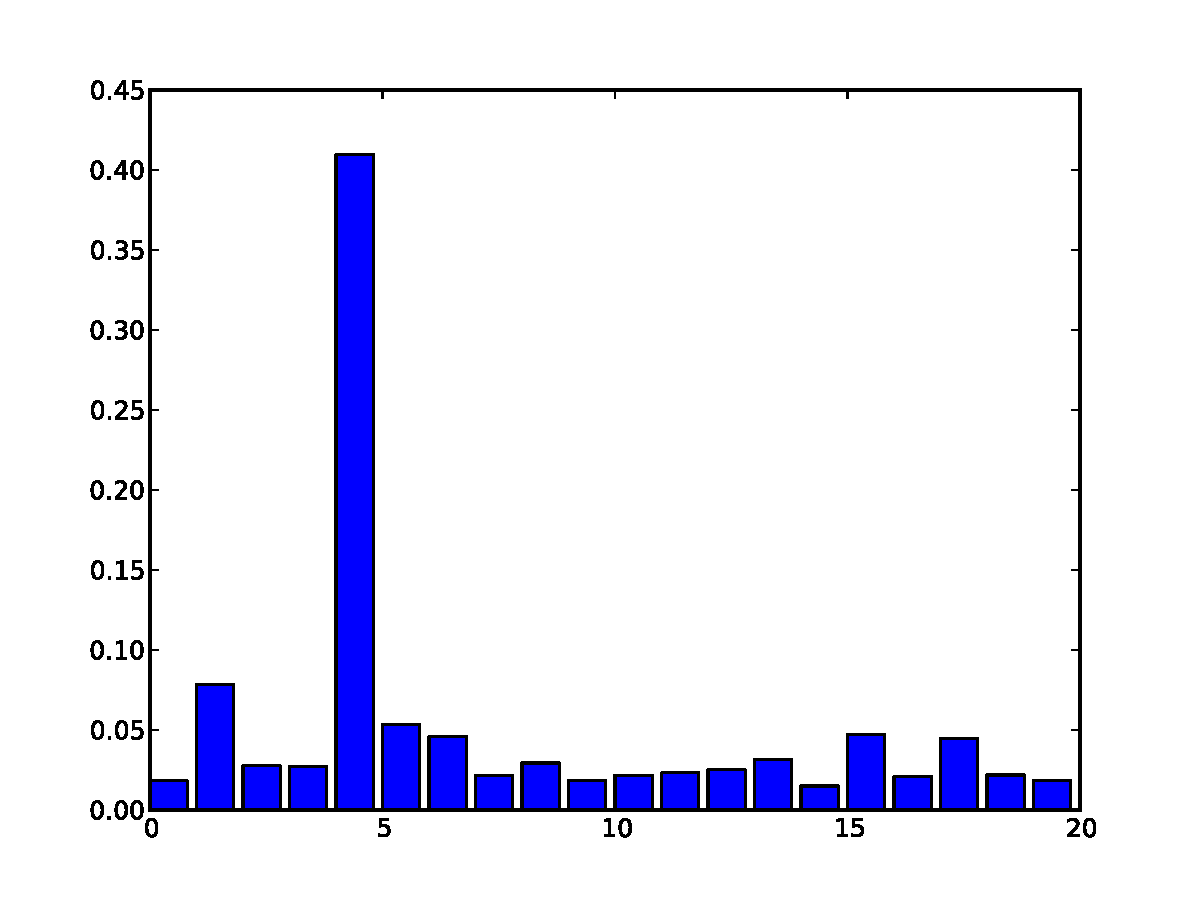
\includegraphics[width=\barw\textwidth]{visualize_dist_paMedLDAgibbs_0/0_1} &
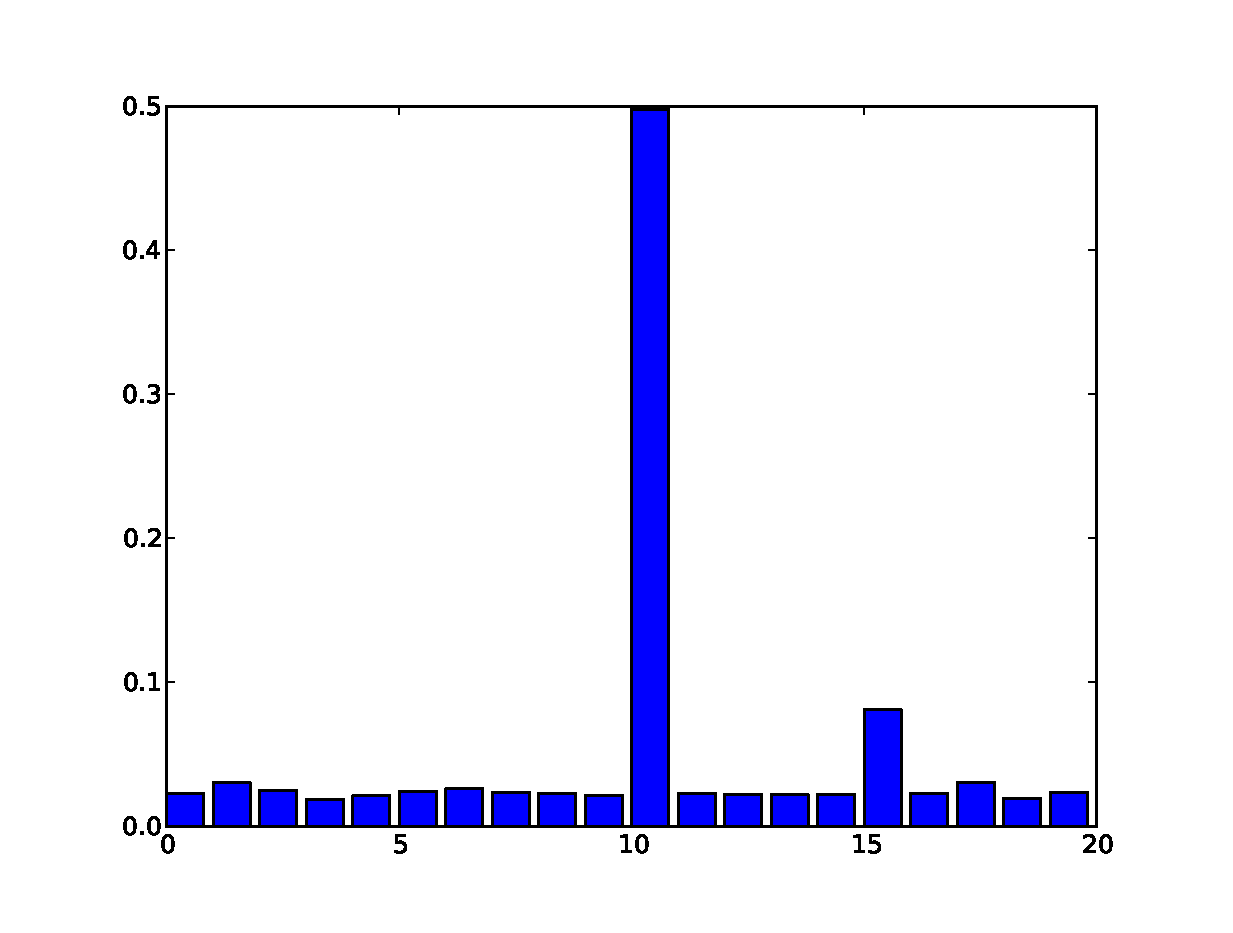
\includegraphics[width=\barw\textwidth]{visualize_dist_paMedLDAgibbs_0/0_8} &
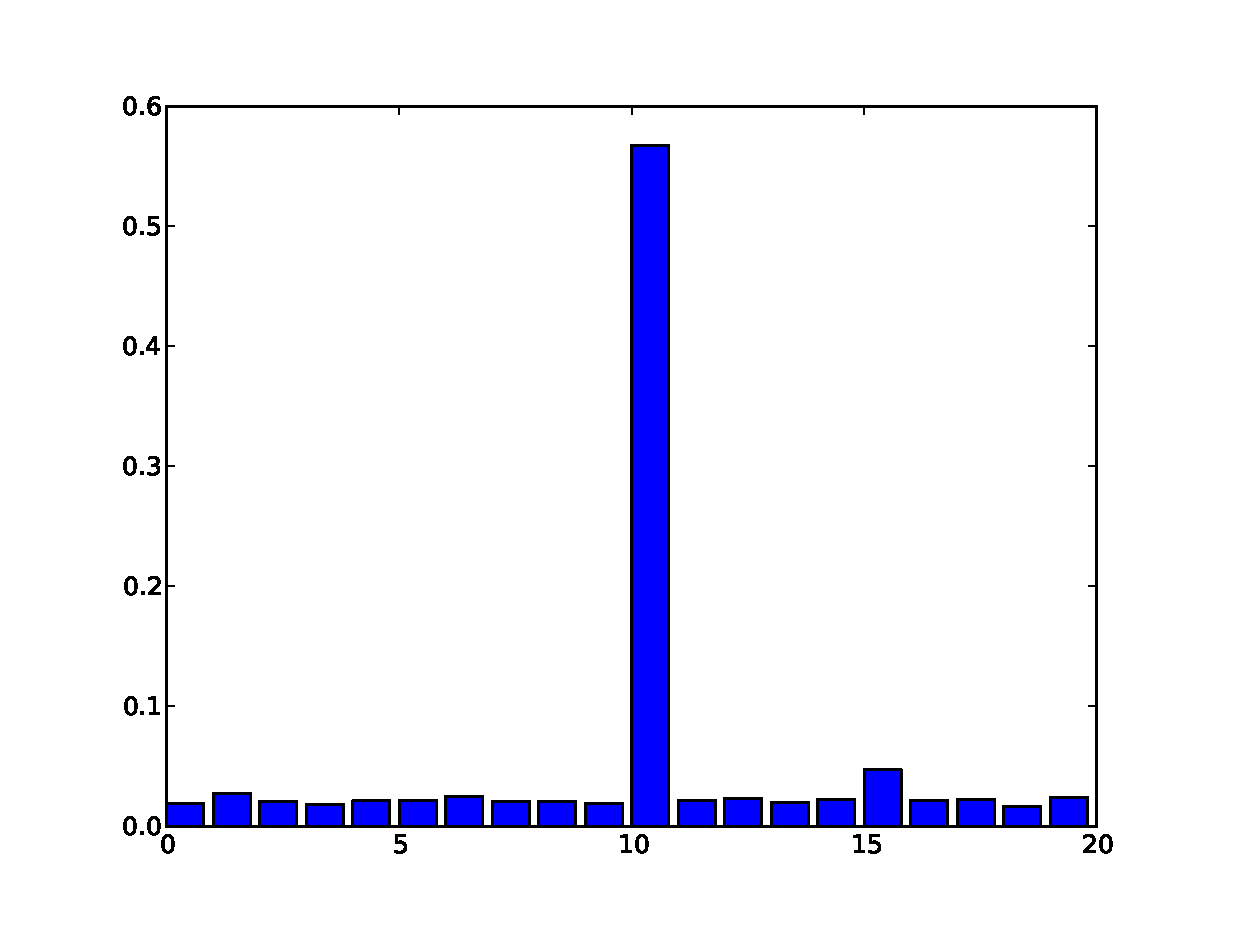
\includegraphics[width=\barw\textwidth]{visualize_dist_paMedLDAgibbs_0/0_22} \\
\hline
\end{tabular} \\

& Top words &
\begin{tabular}{r|cccccc}
 T11 & god & people & writes & article & don & time \\
 T16 & god & people & don & writes & jesus & time
\end{tabular}
\\


\hline

\multirow{6}{*}{comp.graphics} &
\#Observation &
\begin{tabularx}{0.6\textwidth}{XXXXX}
 1 & 64 & 512 & 4096 & 11269 \\
\end{tabularx} \\

& Topic distribution &
\begin{tabular}{ccccc}
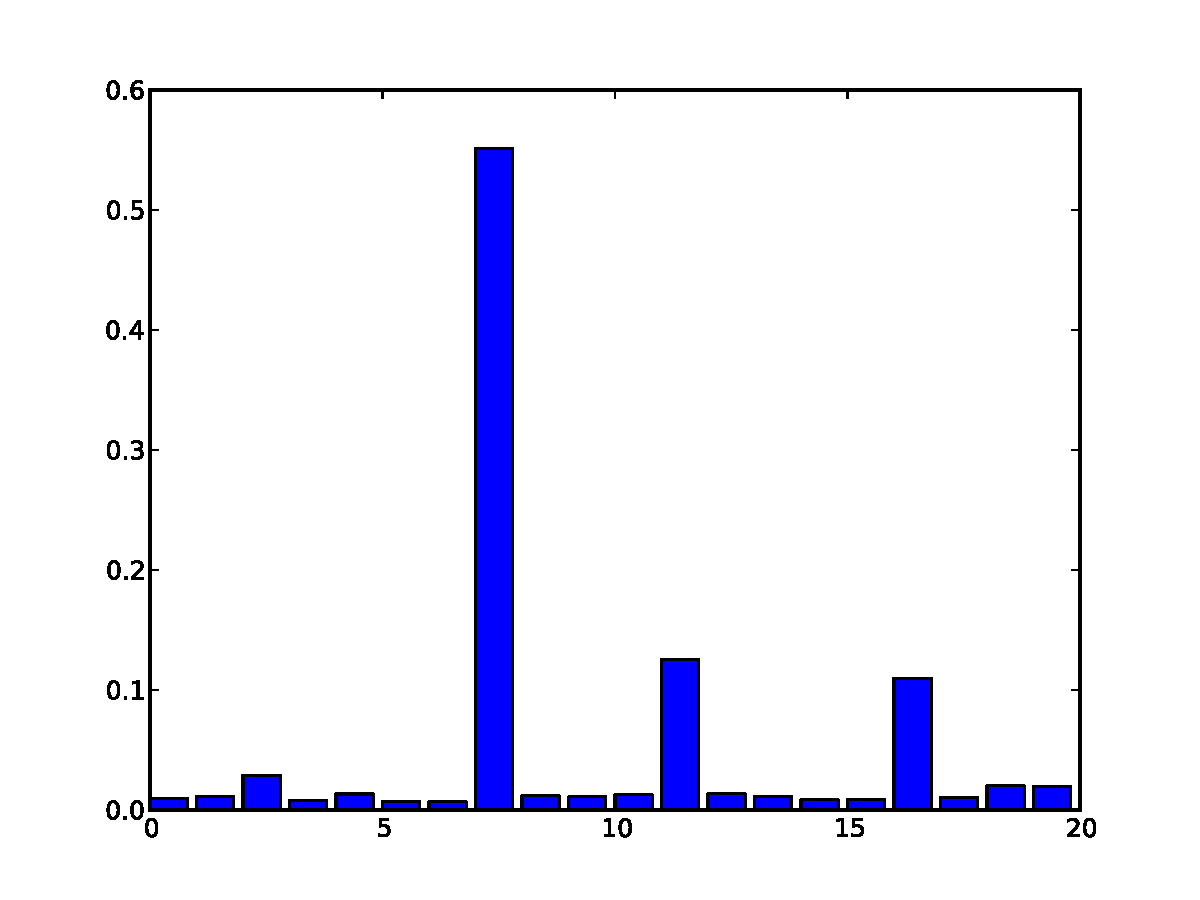
\includegraphics[width=\barw\textwidth]{visualize_dist_paMedLDAgibbs_1/1_0} &
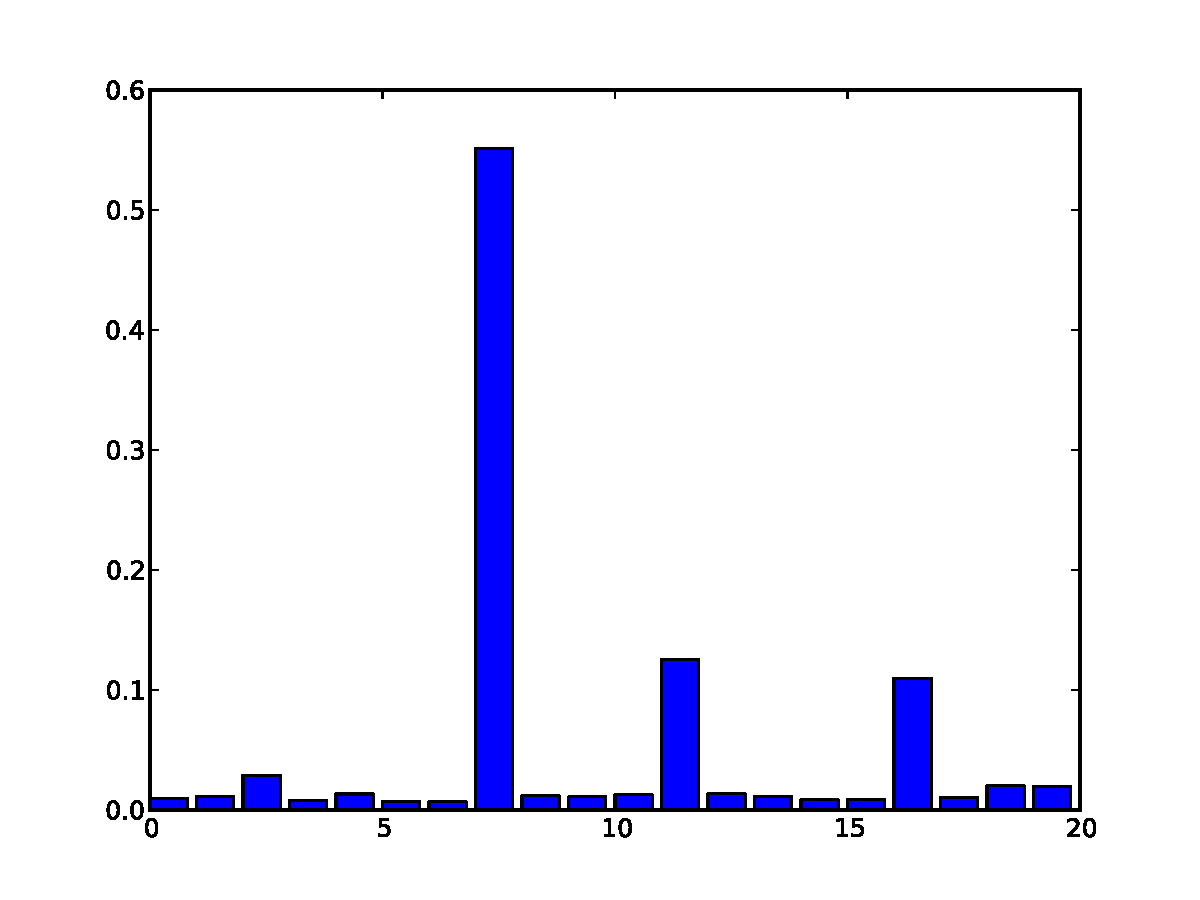
\includegraphics[width=\barw\textwidth]{visualize_dist_paMedLDAgibbs_1/1_0}
&
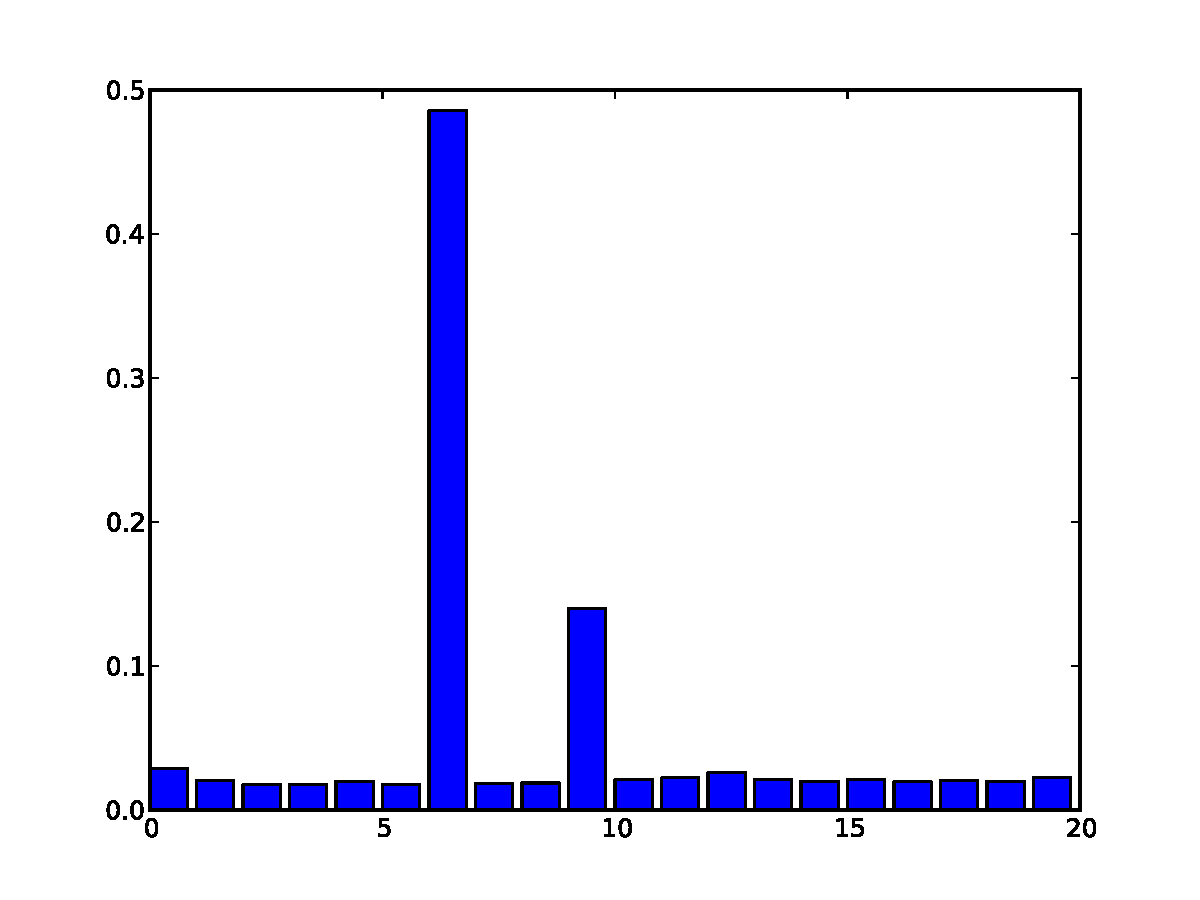
\includegraphics[width=\barw\textwidth]{visualize_dist_paMedLDAgibbs_1/1_1} &
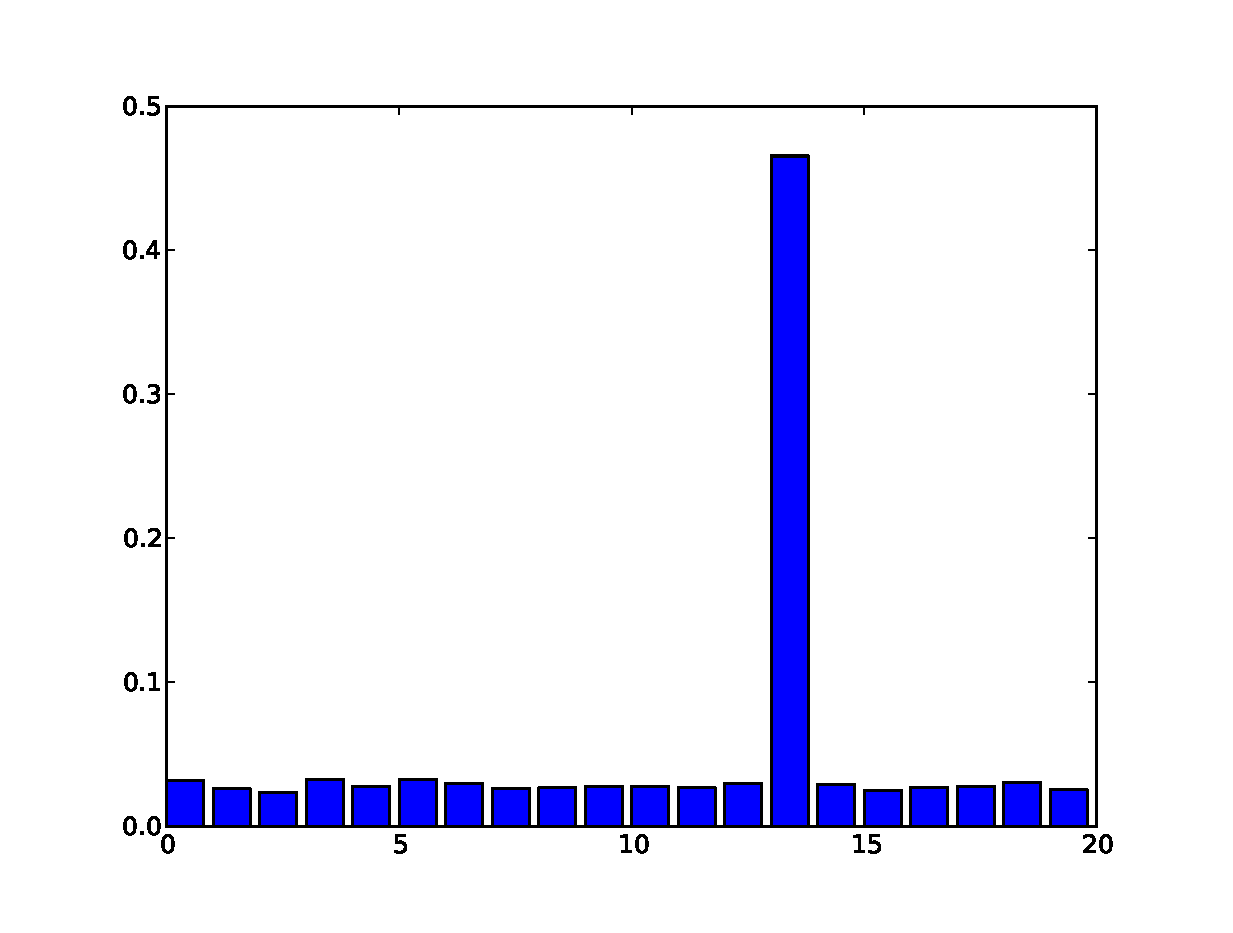
\includegraphics[width=\barw\textwidth]{visualize_dist_paMedLDAgibbs_1/1_8} &
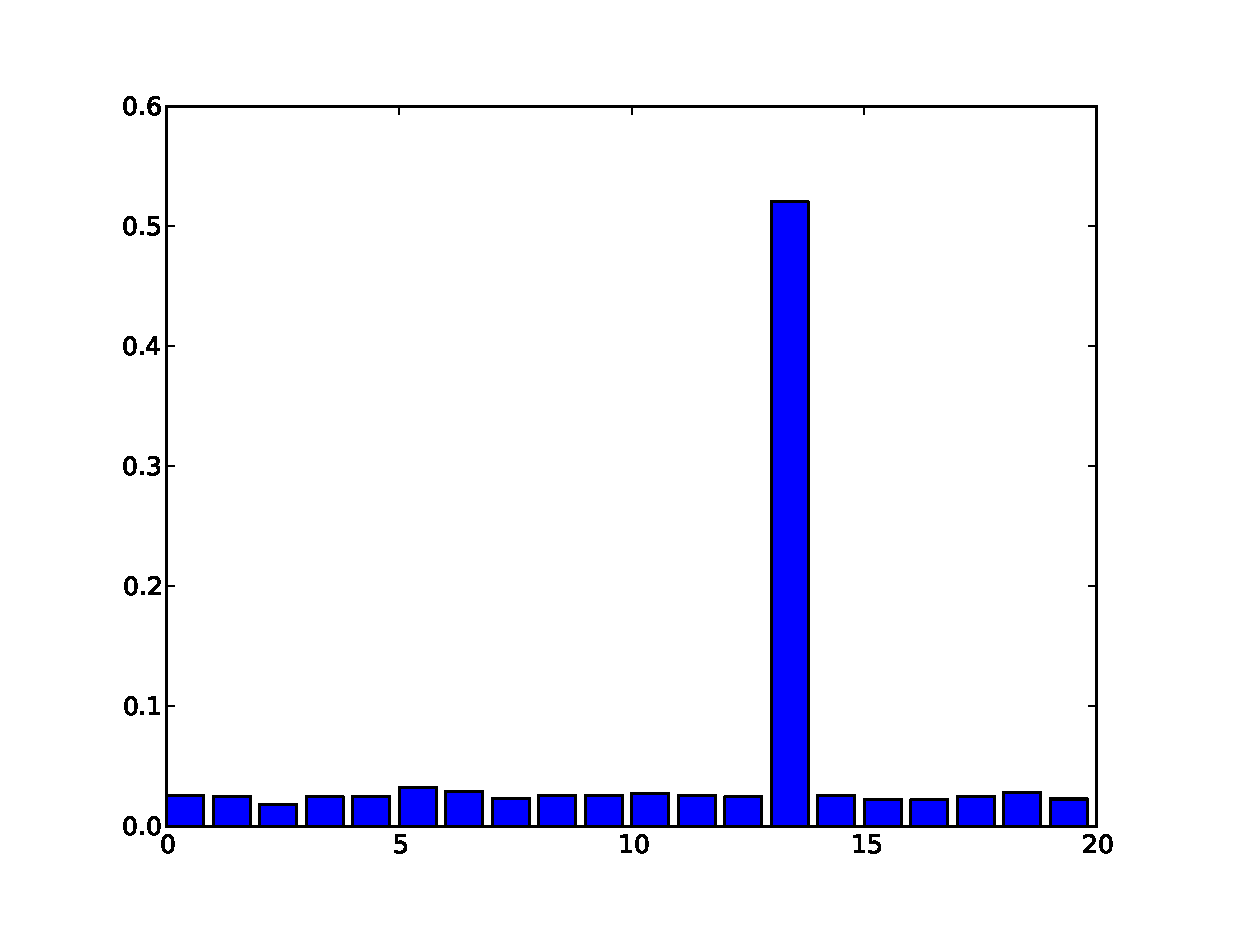
\includegraphics[width=\barw\textwidth]{visualize_dist_paMedLDAgibbs_1/1_22} \\
\hline
\end{tabular} \\

& Top words &
\begin{tabular}{r|cccccc}
 T14 & graphics & image & file & program & images & writes \\
 T13 & entry & space & don & people & system & writes
\end{tabular}
\\

\hline

\multirow{6}{*}{misc.forsale} &
\#Observation &
\begin{tabularx}{0.6\textwidth}{XXXXX}
 1 & 64 & 512 & 4096 & 11269 \\
\end{tabularx} \\

& Topic distribution &
\begin{tabular}{ccccc}
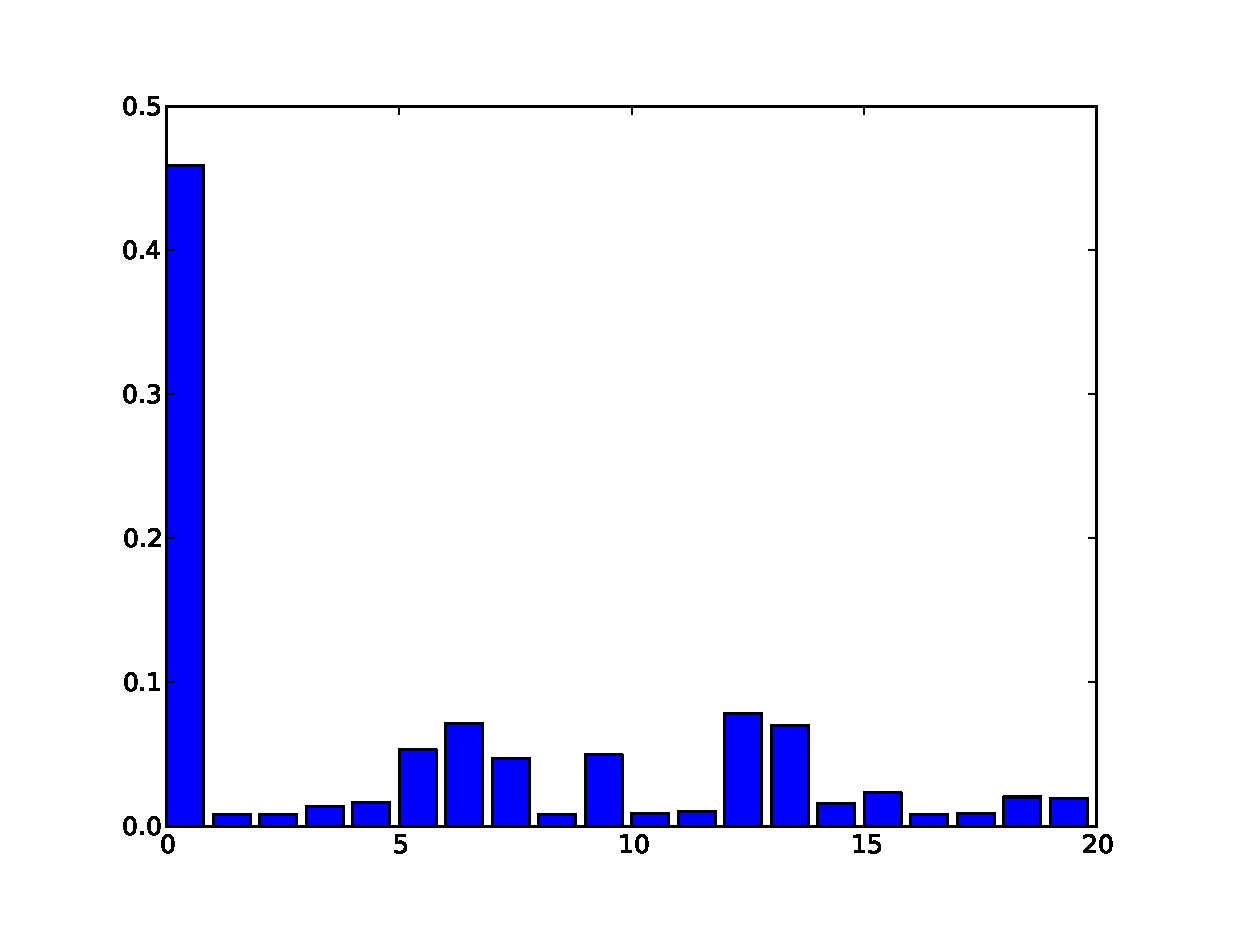
\includegraphics[width=\barw\textwidth]{visualize_dist_paMedLDAgibbs_6/6_0} &
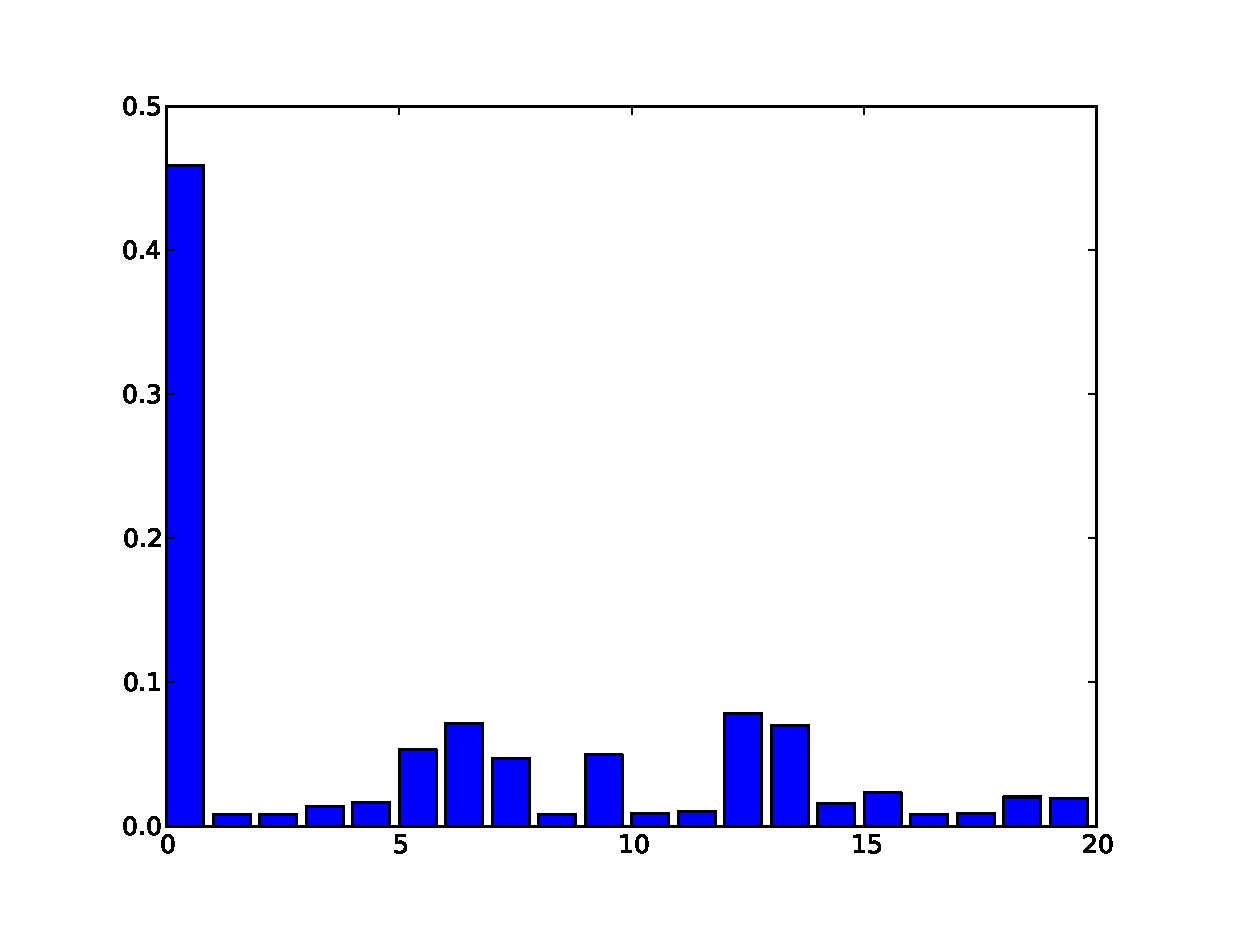
\includegraphics[width=\barw\textwidth]{visualize_dist_paMedLDAgibbs_6/6_0}
&
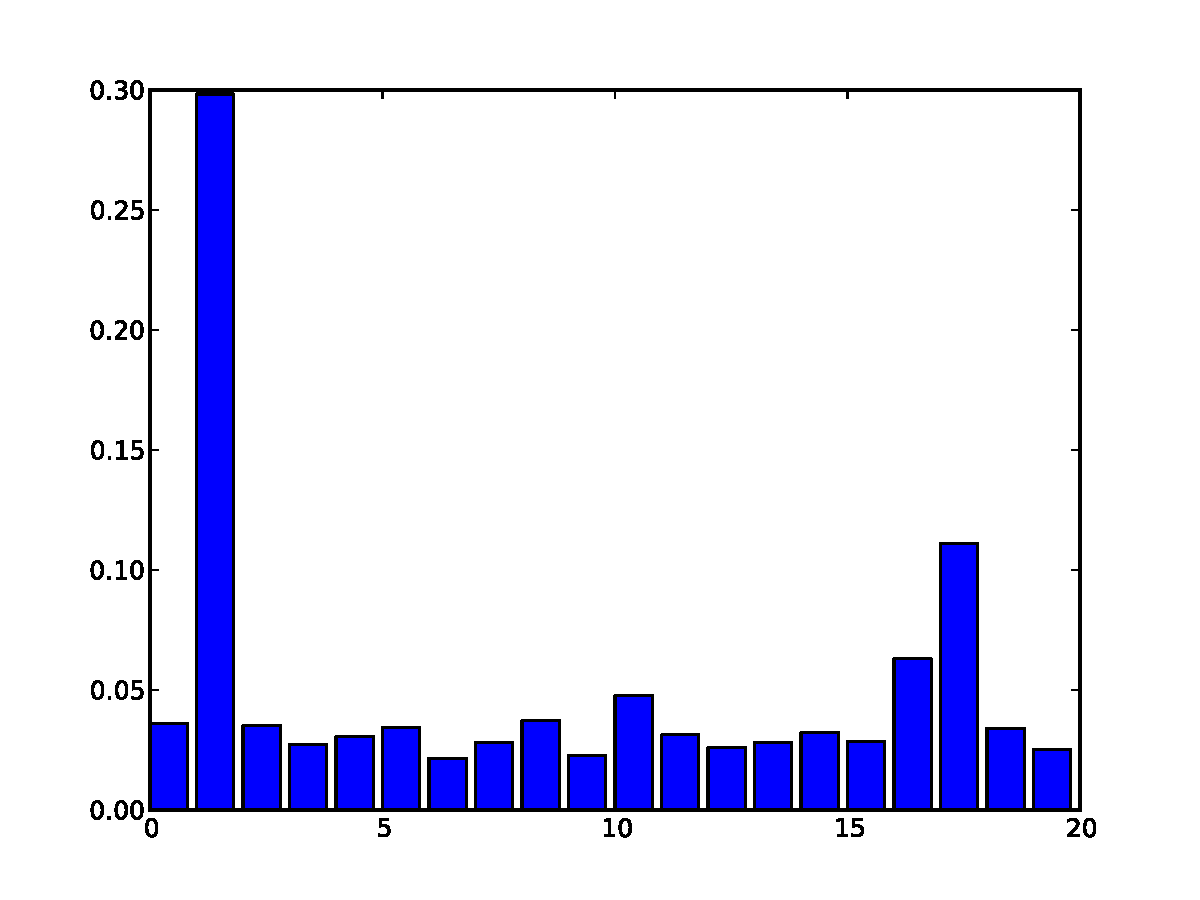
\includegraphics[width=\barw\textwidth]{visualize_dist_paMedLDAgibbs_6/6_1} &
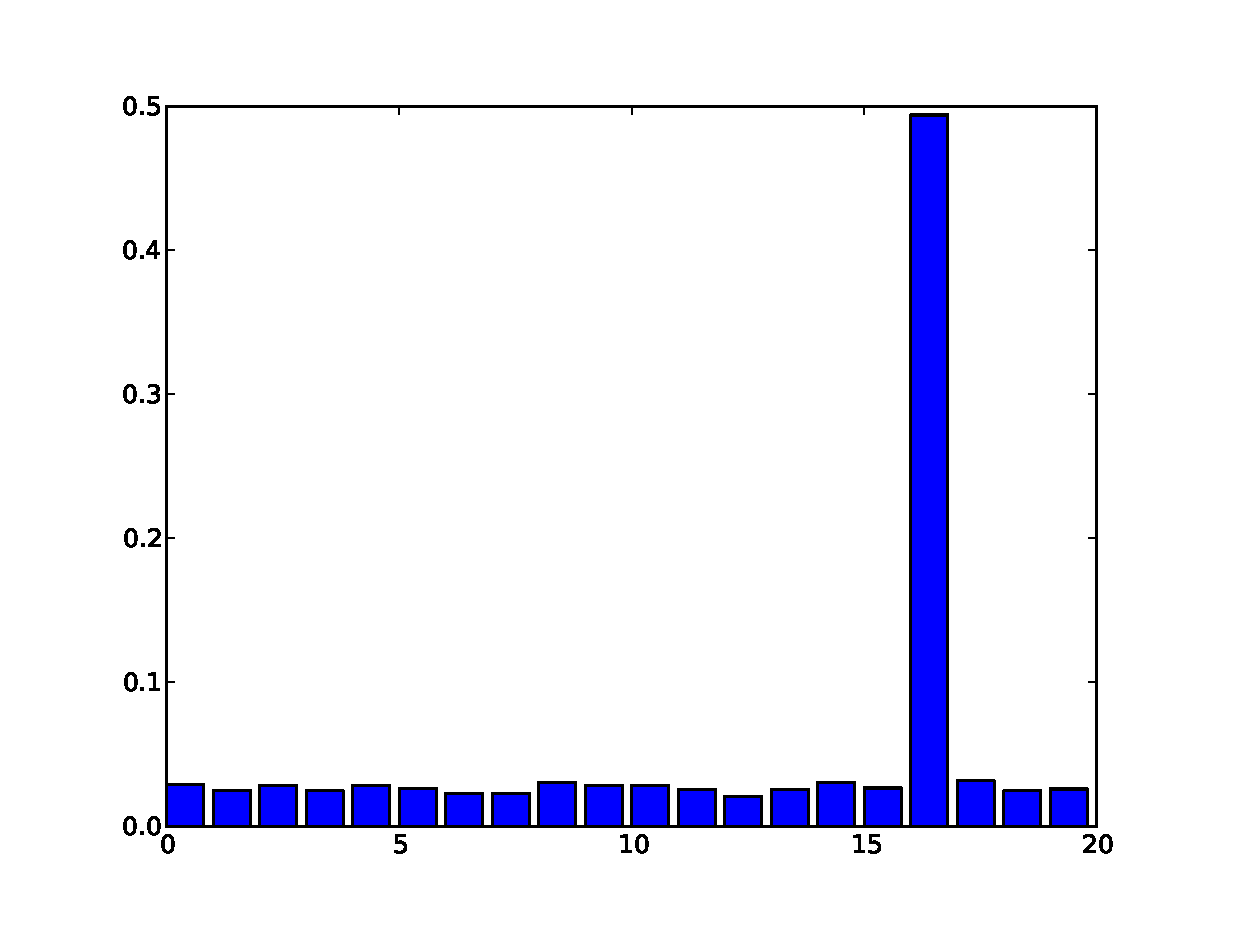
\includegraphics[width=\barw\textwidth]{visualize_dist_paMedLDAgibbs_6/6_8} &
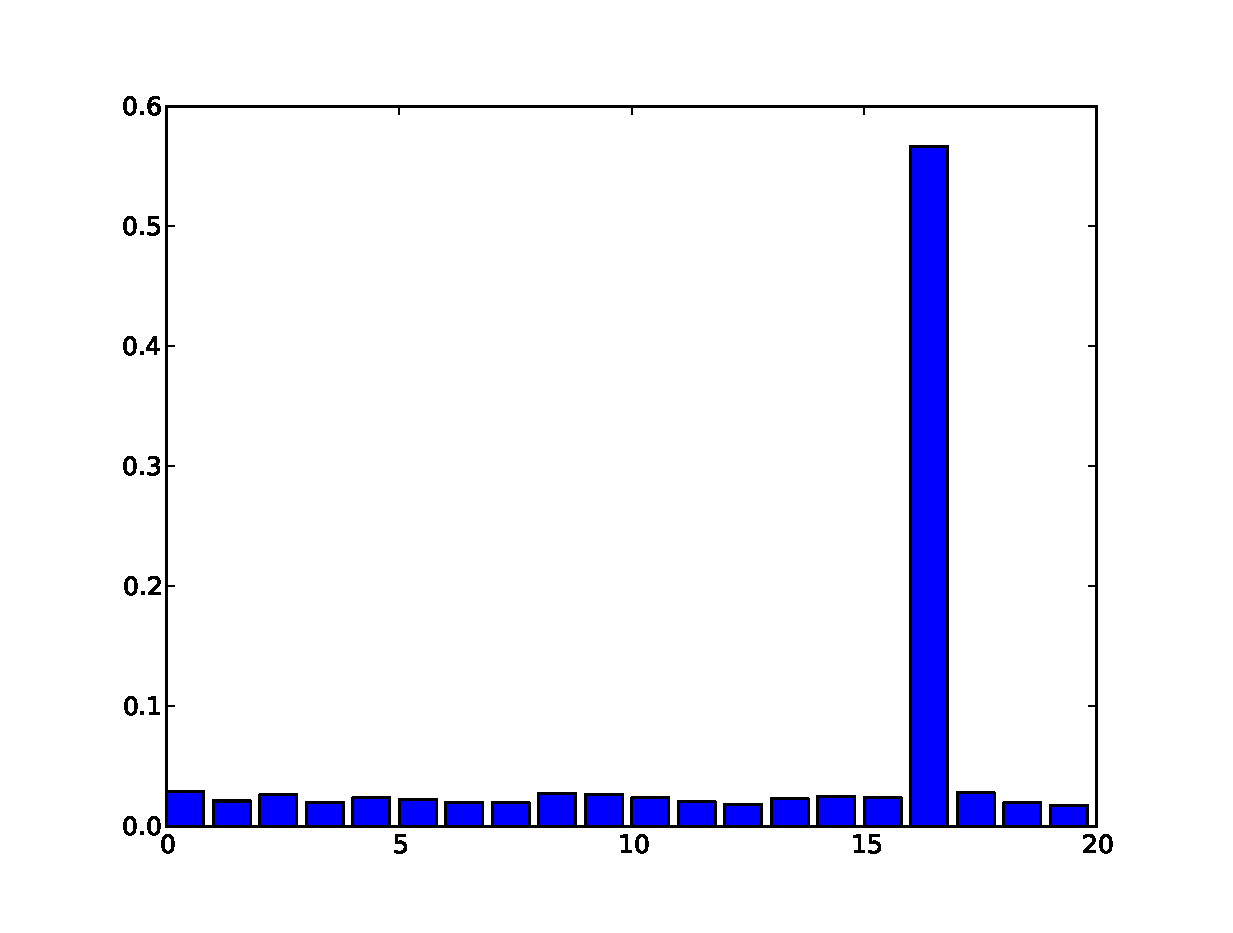
\includegraphics[width=\barw\textwidth]{visualize_dist_paMedLDAgibbs_6/6_22} \\
\hline
\end{tabular} \\

& Top words &
\begin{tabular}{r|cccccc}
 T17 & sale & mail & dos & good & offer & shipping \\
 T18 & don & writes & article & time & good & work
\end{tabular}
\\


\hline\hline
\end{tabular} }
\end{center}\vspace*{-0.2cm}
\caption{Visualization of the learnt topics by \paMedLDAave and \paMedLDAgibbs. See text for details.}\vspace{-.3cm}
\label{tb:visualization_gibbs}
\end{table}


Table \ref{tb:visualization_gibbs} visualizes the learnt topic representation by \paMedLDAave and \paMedLDAgibbs. For the displayed categories, we plot the corresponding classifier's topic distribution averaged over the positive examples and top words from the topic matrix. As we can see, the average topic distributions become increasingly sparse as more and more data are observed. Eventually, the averaged topic distribution for each category contains only 1$\sim$2 non-zero entries and meanwhile different categories have quite diverse average topic distributions, therefore showing strong discriminative ability of the topic representations in distinguishing different categories. Such sparse and discriminatrive patterns are similar to what have been shown in batch settings~\citep{zhu2012medlda, zhugibbs2013}.

% The result is produced using burn-in steps $\mathcal{M} = 10$ for bMedHDP, number of passes $\mathcal{E} = 10$ for tfHDP and a single pass for paMedHDP.

%Comparing Figure \ref{fg:multic_topic_lda} and Figure \ref{fg:multic_topic_hdp}, we could see the test accuracies of paMedLDA and paMedHDP are close, while paMedHDP requires less time to train given the same number of topics. A possible explanation is that paMedHDP handles fewer topics at the first several iterations, and hence becomes faster.

%One more thing to notice is the preferable number of topics. As shown in Figure \ref{fg:multic_topic_lda}, the performance of MedLDA varies little for a large interval of \#topics (for example $K \in [20, 110]$). Therefore, any topic number $K$ in that interval is preferable by an MedHDP model. From Figure \ref{fg:multic_topic_hdp}, we see that paMedHDP infers around 23 topics, while the batch counterparts



\subsection{Extensions}

We now present the experimental results on the extensions of BayesPA topic models. We first present the results of nonparametric topic modeling on the same 20NG data set. Then we demonstrate multi-task learning on a large Wikipedia data set with more than 1 million documents and about 1 million unique terms.





\subsubsection{Nonparametric Topic Modeling}

Recall the nonparametric extensions of BayesPA topic models \paMedHDPave and \paMedHDPgibbs. To validate the advantage of online learning, we test them against their batch counterparts (i.e., the models \MedHDPave and \MedHDPgibbs) on the 20NG corpus. We also include an unsupervised baseline as comparison model, the truncation-free HDP topic model (tfHDP)~\citep{wang2012truncation}, which is first used to discover the latent topic representations, and then combined with a linear SVM classifier for document categorization. For all HDP-based models, the following parameter setting is used: $\alphav = 5 \cdot \bm{1}, \gammav = 0.5 \cdot \bm{1}$ and $\eta = 1$. As an initial number of topic numbers for HDP to start with, we choose $K = 20$. We observed that the training time and the prediction accuracy do not depend heavily on the initial number of topics. The other parameters of BayesPA are the same.

%\jun{how about other K values? Does the time depend on K heavily?} \strin{no}

Figure~\ref{fg:multic_commit} shows the convergence of \paMedHDPave and \paMedHDPgibbs, and Figure~\ref{fg:multic_topic_lda} plots the accuracy and time together with the inferred topic numbers, where the length of the horizontal bars represents the variance of the inferred topic numbers. The results are summarized from five different runs. As we can see, the nonparametric extensions of BayesPA topic models also dramatically improve time efficiency and converge to their batch counterparts in prediction performance. Furthermore, the averaging models are again faster to train because they do not need to update the covariance matrix of classifier weights.





\subsubsection{Multi-Task Classification}



We test \paMedLDAmtave, \paMedLDAmtgibbs and their nonparametric exentions on a large Wiki data set. The Wiki data set is built from the Wikipedia set used in PASCAL LSHC challenge 2012 \footnote{See http://lshtc.iit.demokritos.gr/.}. The Wiki data set is a collection of documents with labels up to 20 different kinds, while the data distribution among the labels is balanced. The training set consists of 1.1 millions of wikipedia documents and the testing test consists of 5,000 documents. The vocabulary contains 917,683 unique terms.
To measure performance, we use F1 score, the harmonic mean of precision and recall.

As baseline batch algorithms, we include MedLDAmt, a recent multi-task extention of Gibbs MedLDA~\citep{zhu2013scalable}. Since MedHDP is a new model, there is no exising implementation of multi-task batch versions. So we instead extended MedHDP to support multi-task inference. We call this model MedHDPmt.

We use the same validation scheme as previous to select batchsize $|B| = 1, c = 5000, \sigma^2 = 10^{-6}$ for \paMedLDAmtave; We choose $|B| = 512, c = 1, \sigma^2 = 1$ for \paMedLDAmtgibbs. For both models, the Dirichlet parameters are $\alphav = 0.8 \cdot \bm{1}, \gammav = 0.5 \cdot \bm{1}$,  and $\epsilon = 1$. We use $K = 40$ topics for MedLDA models. The nonparametric extensions use exactly the same parameter settings except that $\alphav = 5 \cdot \bm{1}, \eta = 1$ and we do not need to specify the topic number $K$.

\begin{figure}[t]
\centering
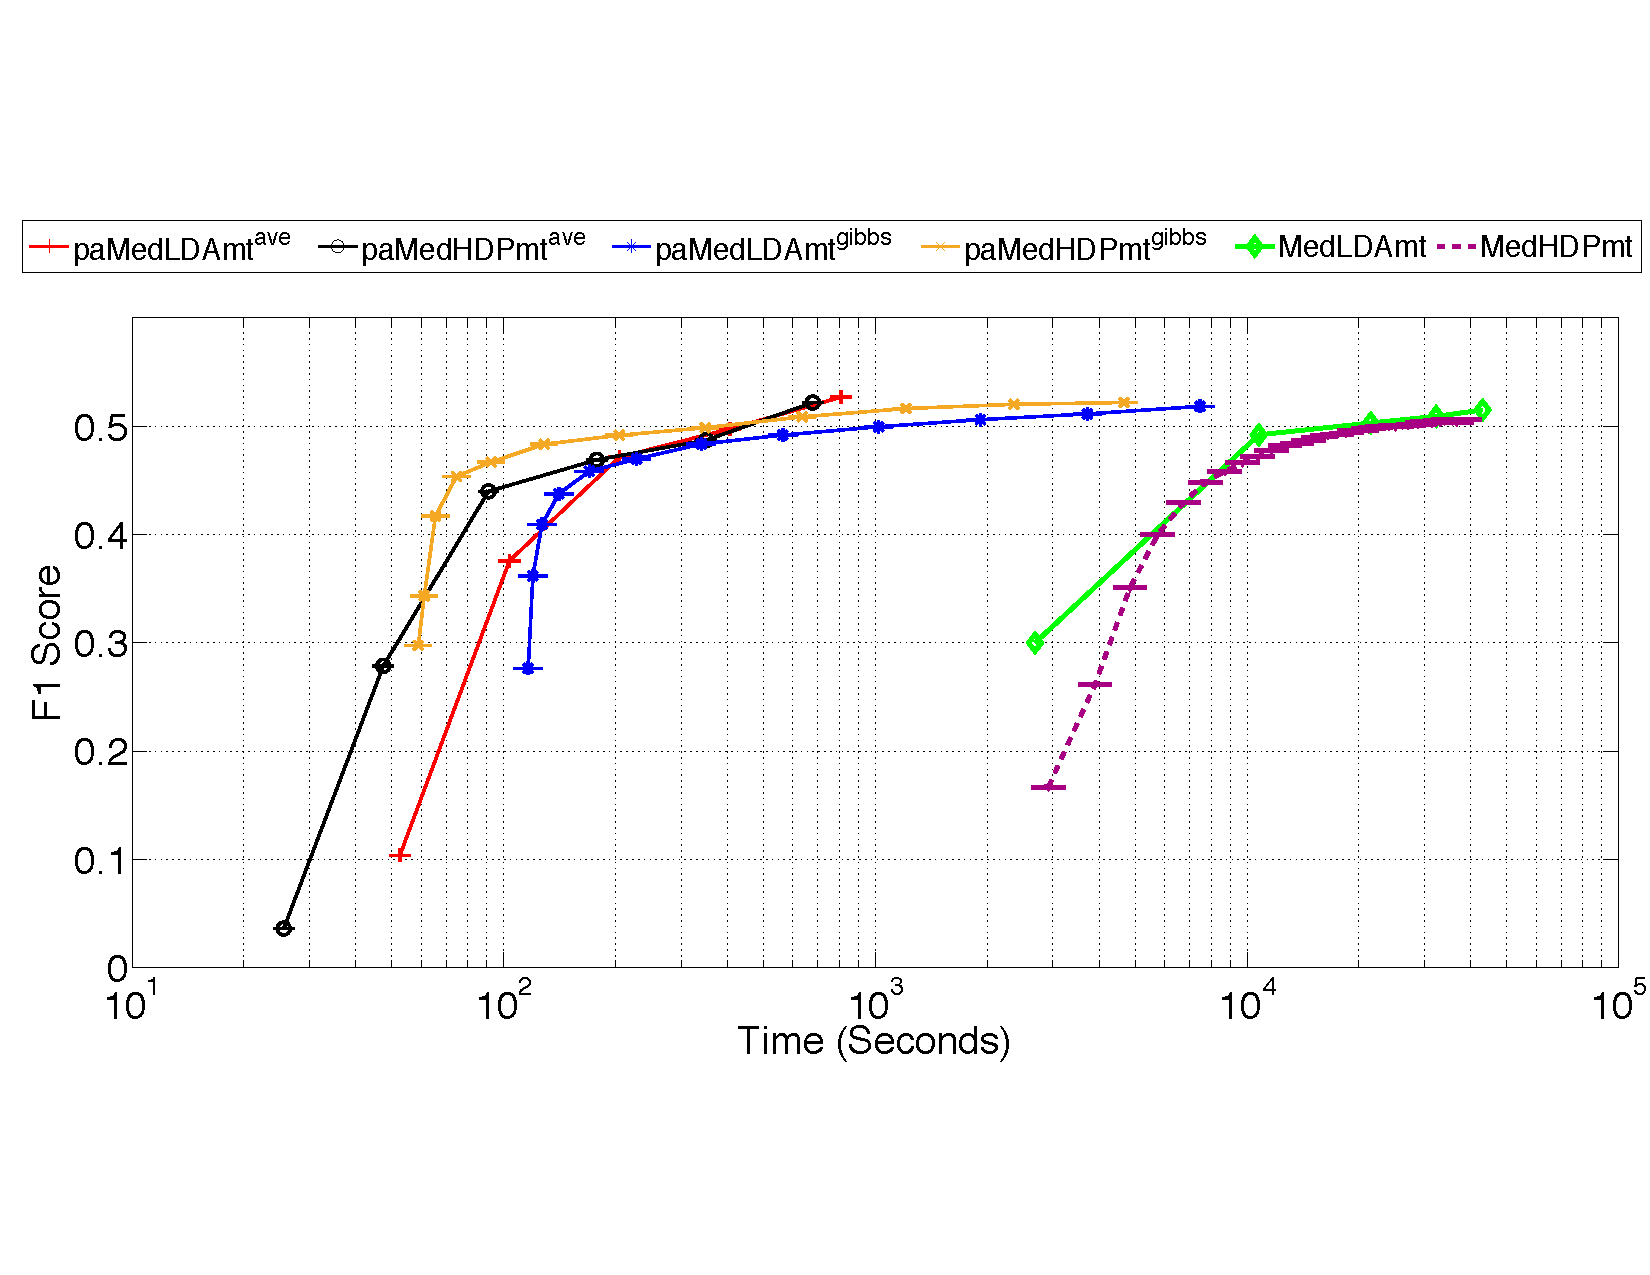
\includegraphics[width = 0.9\textwidth]{plot_mtask_commit_jmlr.pdf}
\vspace*{-0.2cm}
\caption{F1 scores of various multi-task topic models with respect to the running time on the 1.1M wikipedia data set.}
\vspace*{-0.4cm}
\label{fg:multic_mtask_commit}
\end{figure}

Figure \ref{fg:multic_mtask_commit} shows the F1 scores of various models as a function of training time. We find that BayesPA topic models produce comparable results with their batch counterparts, but the training time is significantly less. With either Gibbs or averaging classifiers, BayesPA is about two orders of magnitude faster than their batch counterparts. Therefore, BayesPA topic models could potentially be applied to large-scale multi-class settings.


%In fact, the similarity of multi-task Bayesian PA topic models and multi-task Gibbs MedLDA suggests that a highly paralleled and scalable implementation is possible \citep{zhu2013scalable}.




\subsection{Sensitivity Analysis}\label{sec:sensitivity}
%\junx{This section should be moved to the end of the experiments since you're using the nonparametric models.}

We provide further discussions on BayesPA learning for topic models. We analyze the models' sensitivity to some  key parameters.

%Second, we illustrate an application with a large Wikipedia dataset containing 1.1 million documents, where class labels are not exclusive.
%\label{sec:discuss}

%\subsubsection{Sensitivity Analysis}
%\label{sec:sensitivity}




\textbf{Batch Size $|B|$: } Figure \ref{fg:multic_batchsize} presents the test errors of BayesPA topic models (\paMedLDAave, \paMedLDAgibbs) as a function of training time on the entire 20NG data set with various batch sizes. The number of topics is fixed at $K = 40$. We can see that the convergence speeds of different algorithms vary. First of all, the batch algorithms suffer from multiple passes through the data set and therefore are much slower than the online alternatives. Second, we could observe that algorithms with medium batch sizes ($|B| = 64$ or $256$) converge faster. If we choose a batch size too small, for example, $|B| = 1$, each iteration would not provide sufficient evidence for the update of global variables; if the batch size is too large, each mini-batch becomes redundant and the convergence rate also decreases. By comparing the two figures, we find that \paMedLDAave runs faster than \paMedLDAgibbs. This is because for averaging classifers, we do not update the covaraince of the classifier weights, which requires frequent matrix inverse operations. Furthermore, \paMedLDAave appears to be more robust against change in batchsize. Similarly, Figure \ref{fg:multic_batchsize_hdp} shows the sensitivity experiment of the batchsize parameter in paMedHDP models. The results are similar to paMedLDA models, that is, a moderate batchsize leads to faster convergence.

\begin{figure}[t]
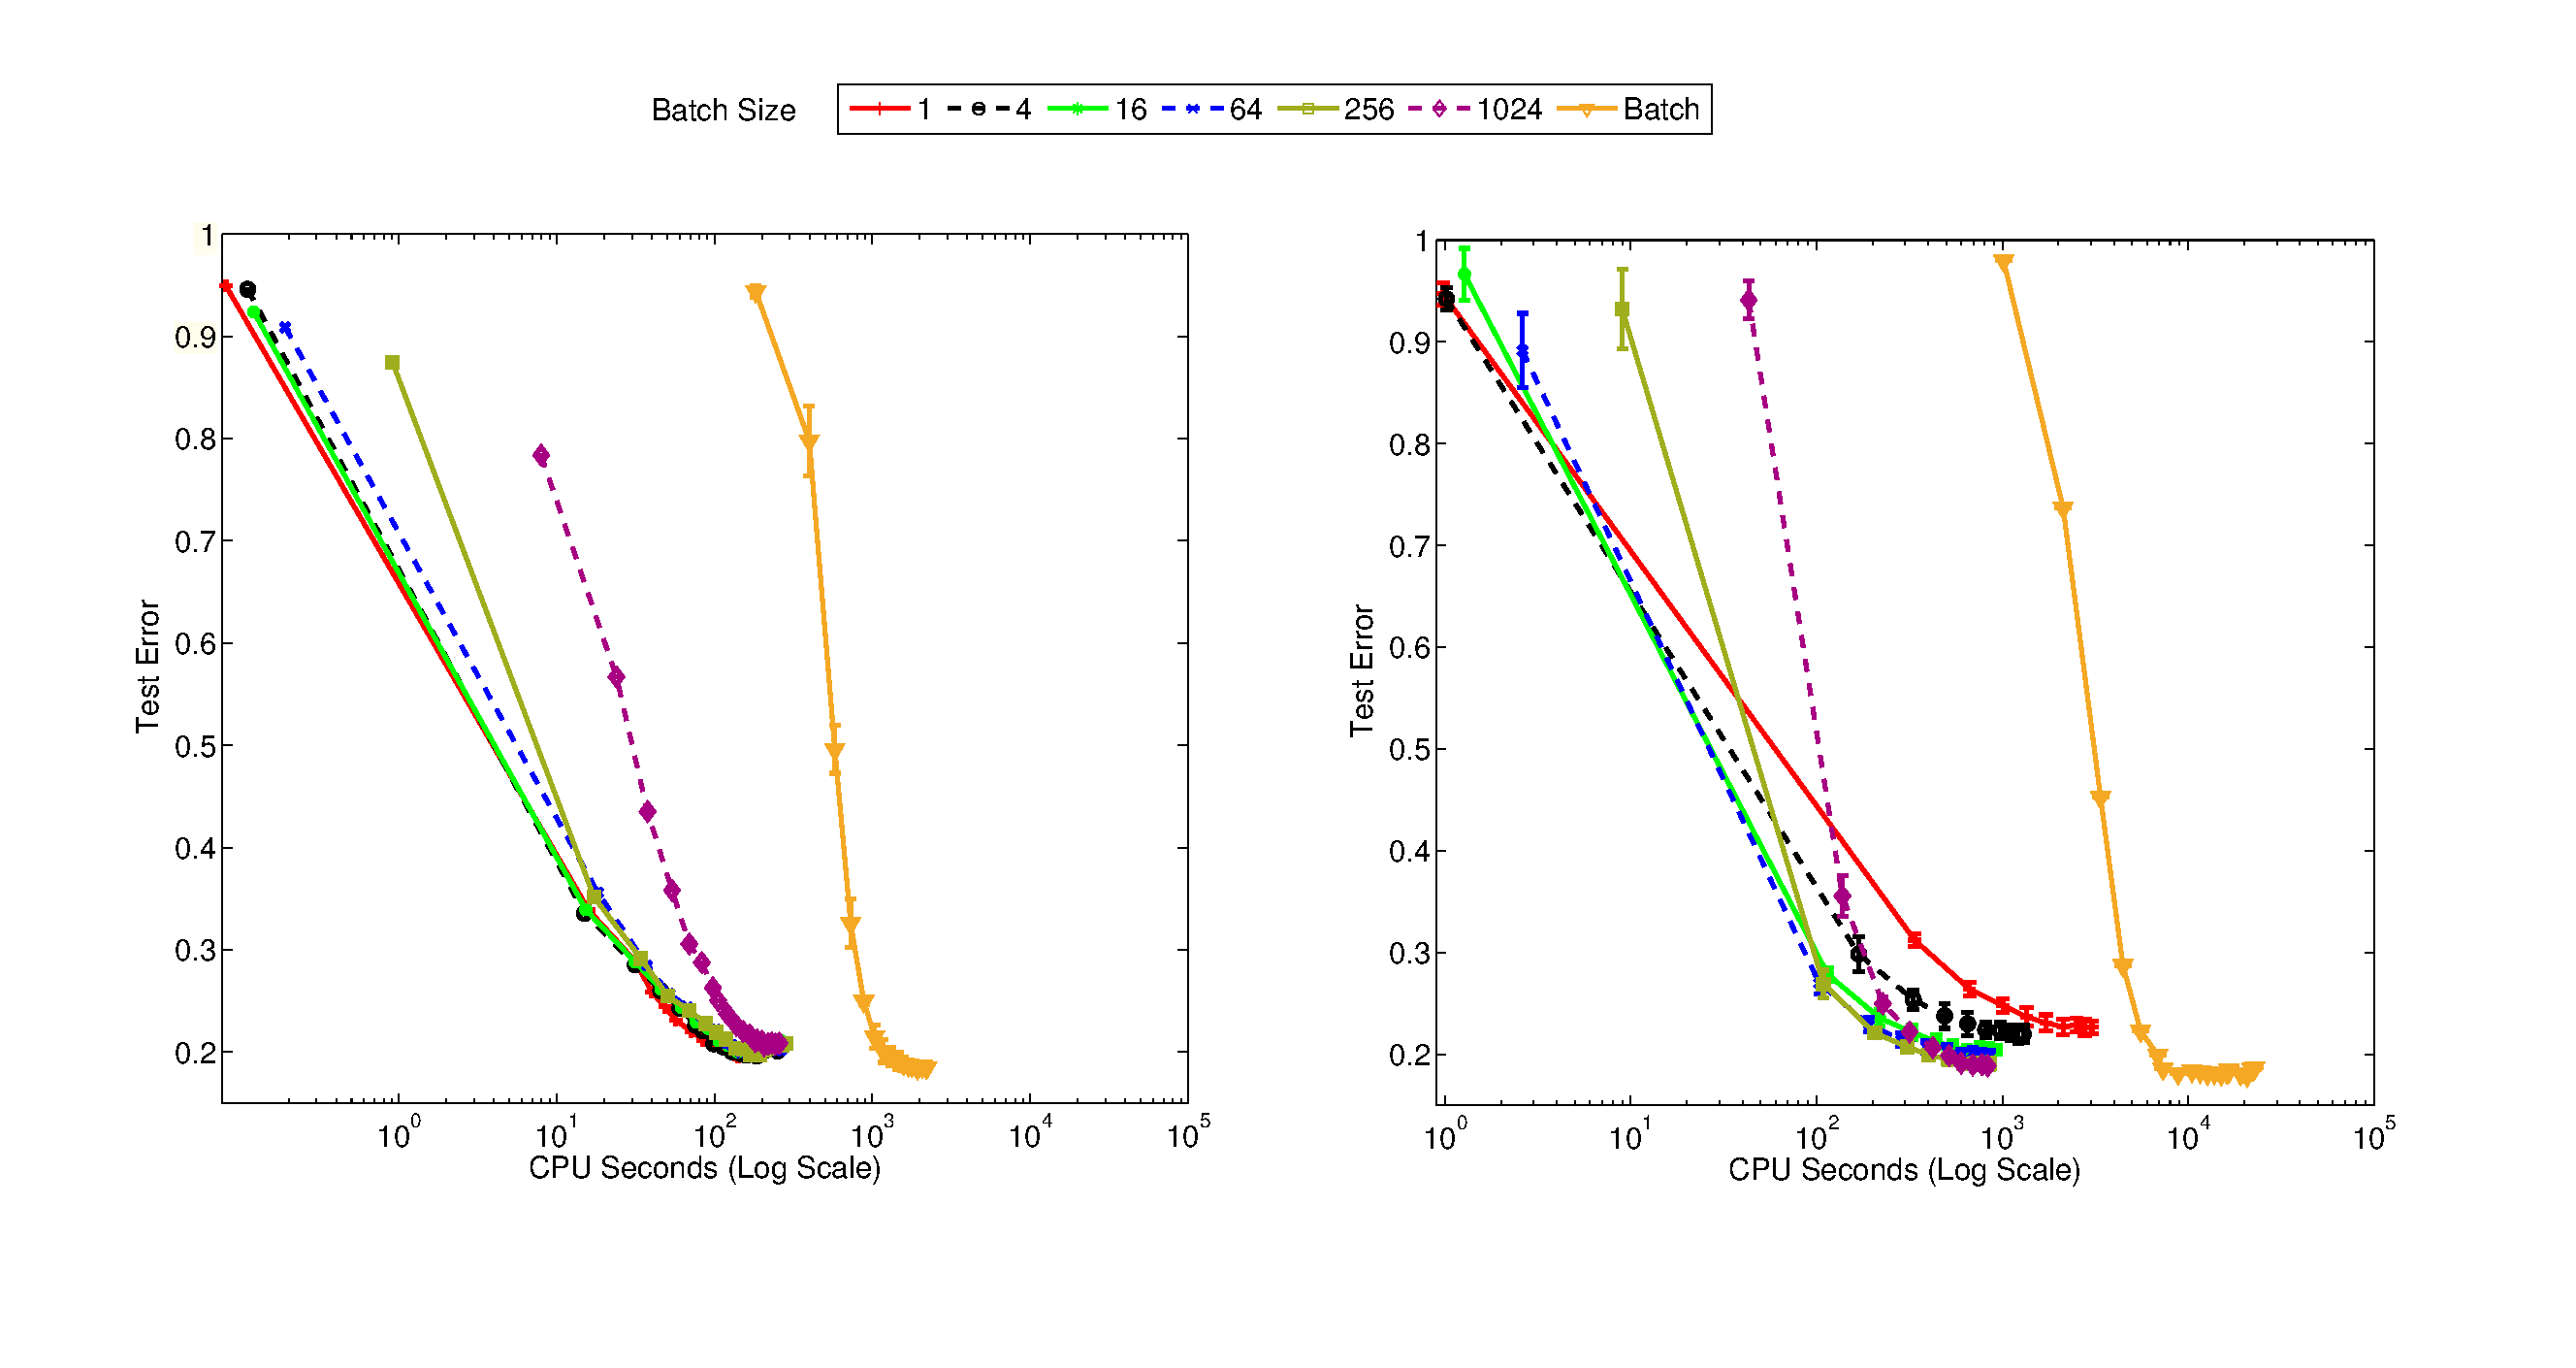
\includegraphics[width = .95\textwidth]{plot_multic_batchsize_jmlr-eps.pdf}\vspace*{-0.2cm}
\caption{Test errors of \paMedLDAave (left) and \paMedLDAgibbs (right) with different batch sizes on the 20NG data set. }
\label{fg:multic_batchsize}\vspace*{-0.4cm}
\end{figure}
\begin{figure}[t]
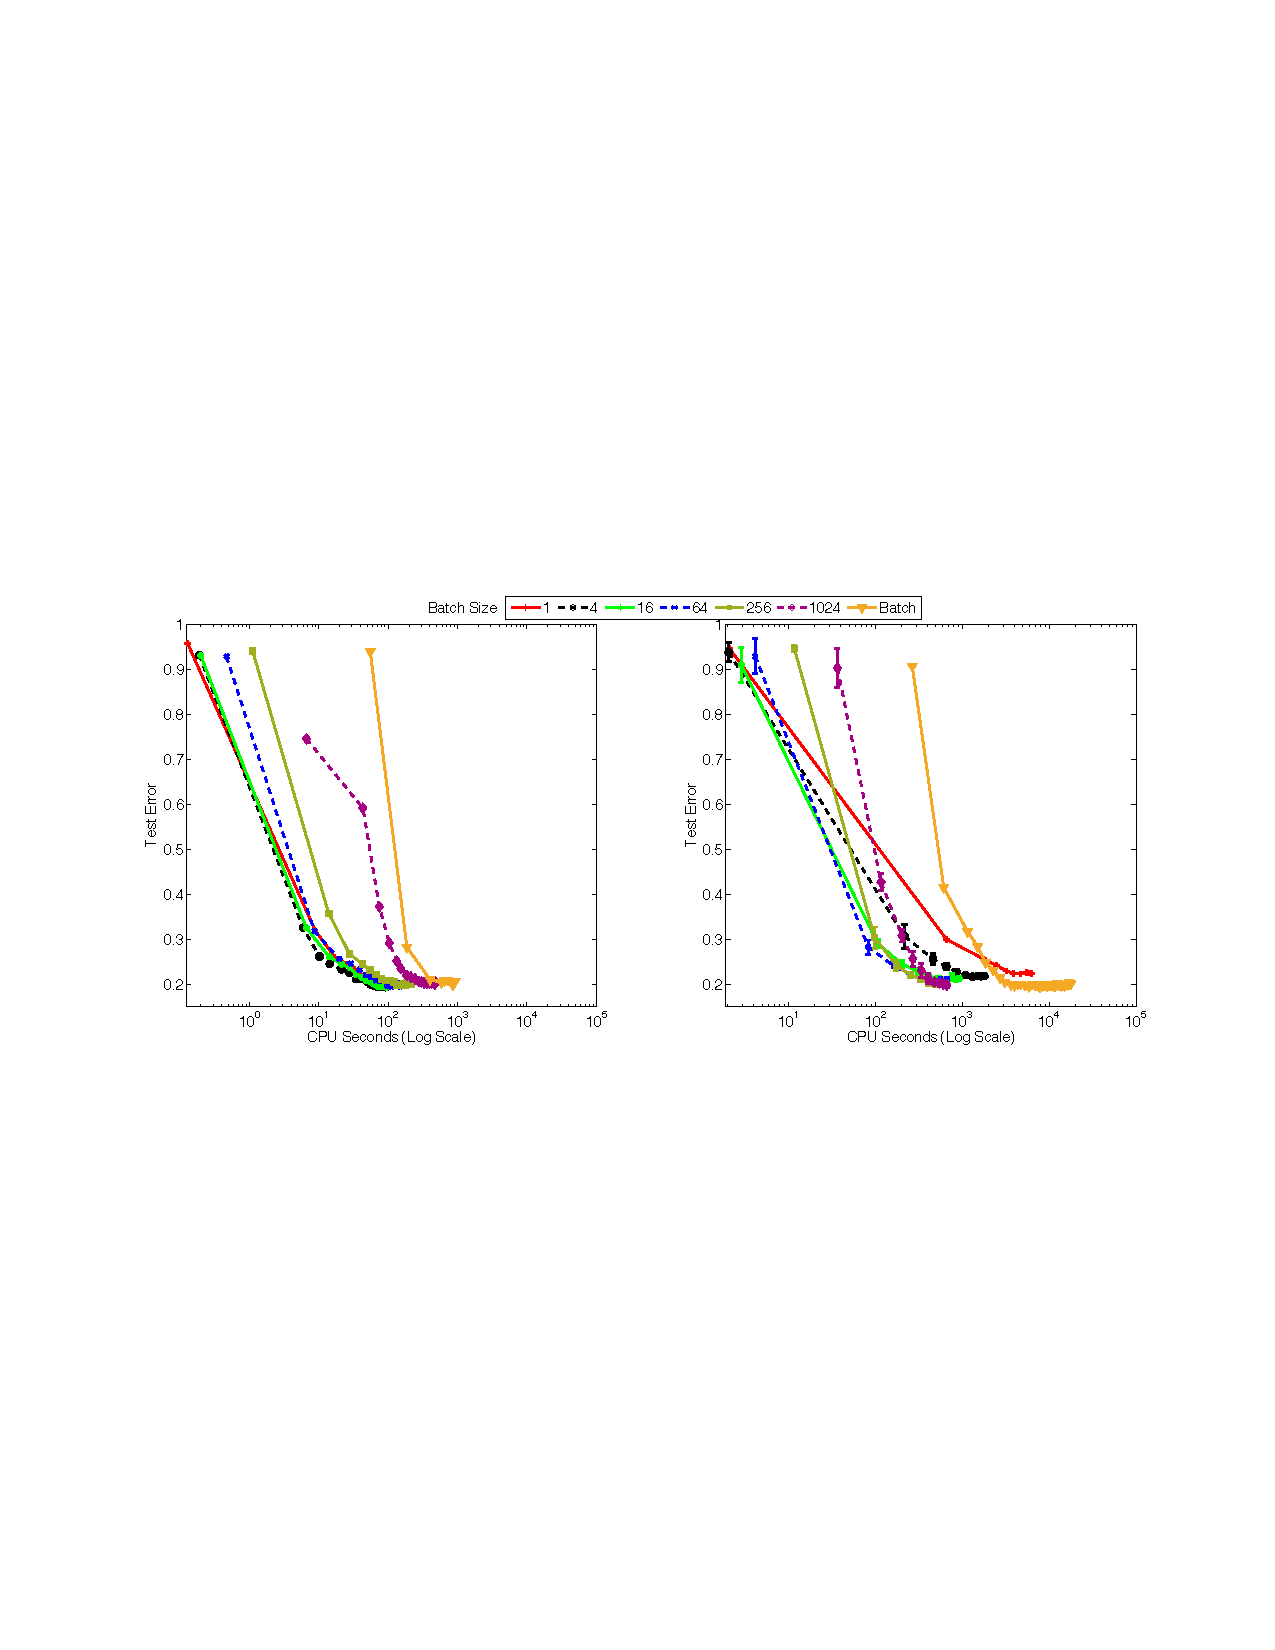
\includegraphics[width = .95\textwidth]{plot_multic_batchsize_hdp_jmlr.pdf}\vspace*{-0.2cm}
\caption{Test errors of \paMedHDPave (left) and \paMedHDPgibbs (right) with different batch sizes on the 20NG data set. }
\label{fg:multic_batchsize_hdp}\vspace*{-0.2cm}
\end{figure}

\begin{figure}[t]
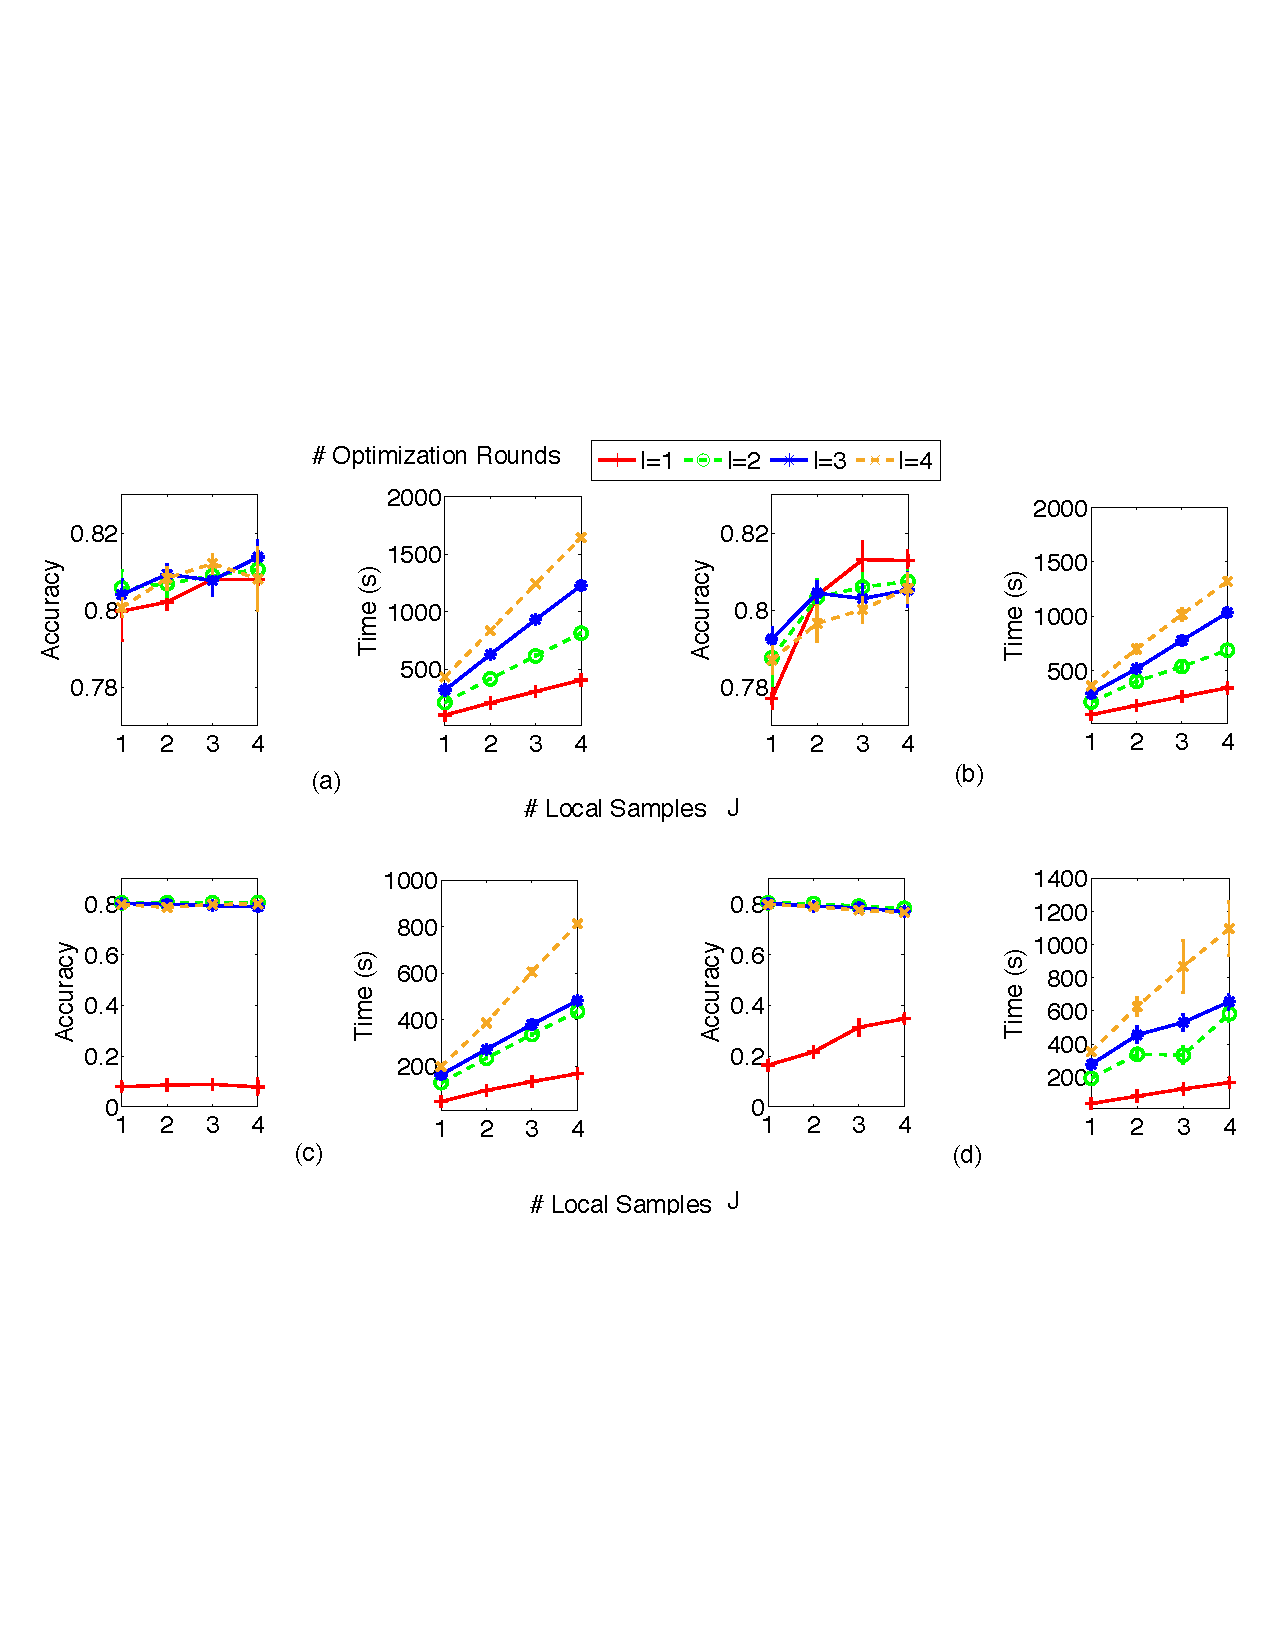
\includegraphics[width = \textwidth]{plot_ij.pdf}
%\vspace*{-0.5cm}
\caption{Classification accuracies and training time of \textbf{(a)}: \paMedLDAgibbs, \textbf{(b):} \paMedHDPgibbs, \textbf{(c)}: \paMedLDAave, and \textbf{(d):} \paMedHDPave, with different combinations of $(\mathcal{I}, \mathcal{J})$ on the 20NG data set. The x-axis includes different values of $\mathcal{J}$, while different values of $\mathcal{I}$ are shown as separate lines. }
\label{fg:multic_IJ}
\end{figure}


\textbf{Number of iterations $\mathcal{I}$ and samples $\mathcal{J}$: } Since the time complexity of Algorithm \ref{algo:pamedlda} is linear in both $\mathcal{I}$ and $\mathcal{J}$, we would like to know how these parameters influence the quality of the trained models.  First, we analyze which setting of $(\mathcal{I}, \mathcal{J})$ guarantees good performance. Fix $\beta = 0, K = 40$.
% for paMedLDAgibbs, we choose batchsize = 512; for paMedLDAave, we choose batchsize = 1.
Figure \ref{fg:multic_IJ} presents the results. % As we can see, for $\mathcal{J} = 1$, the algorithms suffer from the noisy approximation and therefore sacrifices prediction accuracy. But for larger $\mathcal{J}$, simply $\mathcal{I} = 1$ is promising, possibly due to the redundancy among mini-batches.
First, the number of samples $\mathcal{J}$ does not have a large effect on the accuracy. Second, the peformance of \paMedLDAgibbs and \paMedHDPgibbs is not sensitive the number of optimization round, but \paMedLDAave and \paMedHDPave suffers largely if $\mathcal{I} = 1$. This is because with averaging classifiers, the sampling of latent variable $\Zv$ relies not only on global parameters, but also on a local variable $\tau$, so more optimization rounds are needed. The training time of all models scale linearly in terms of $\mathcal{I}$ and $\mathcal{J}$.


% note: The background color of cell is obtained by renormalizing the accuracy into [0.4, 0.8]
\begin{table}[h]
\begin{center}
\begin{tabular}{cc}
\begin{tabular}{c  c  c  c c c }
\backslashbox[5mm]{$\mathcal{J}$}{$\beta$} & 0 & 2 & 4  \\
\hline
1 & \cellcolor[gray]{0.656} 0.802 &\\
3 & \cellcolor[gray]{0.72} 0.803 & \cellcolor[gray]{0.72} 0.803 \\
5  &\cellcolor[gray]{0.75} 0.805 &\cellcolor[gray]{0.75} 0.805 & \cellcolor[gray]{0.72} 0.803 \\
% 9 & \cellcolor[gray]{0.761} 0.806 & \cellcolor[gray]{0.761} 0.806 & \cellcolor[gray]{0.761} 0.806 & \cellcolor[gray]{0.730} 0.804 & \cellcolor[gray]{0.608} 0.796\\
\hline
\end{tabular}
&
\begin{tabular}{c  c  c  c c }
\backslashbox[5mm]{$\mathcal{J}$}{$\beta$} & 0 & 2 & 4 \\
\hline
1 &
\cellcolor[gray]{0.4} 0.783 &\\
3 & \cellcolor[gray]{0.72} 0.803 & \cellcolor[gray]{0.6560} 0.799 \\
5  &\cellcolor[gray]{0.8} 0.808 &\cellcolor[gray]{0.72} 0.803 & \cellcolor[gray]{0.5440} 0.792 \\
% 9 & \cellcolor[gray]{0.761} 0.806 & \cellcolor[gray]{0.761} 0.806 & \cellcolor[gray]{0.761} 0.806 & \cellcolor[gray]{0.730} 0.804 & \cellcolor[gray]{0.608} 0.796\\
\hline
\end{tabular}
 \\
(a) & (b)
\end{tabular}
\end{center}\vspace*{-0.2cm}
\caption{Effect of the number of local samples and burn-in steps for \textbf{(a).} \paMedLDAave; and  \textbf{(b).} \paMedLDAgibbs.}
\label{tb:samplen}\vspace*{-0.2cm}
\end{table}



Notice that the first $\beta$ samples are discarded as burn-in steps. To understand how large $\beta$ is sufficient, we consider the settings of the pairs $(\mathcal{J}, \beta)$ and check the prediction accuracy of Algorithm \ref{algo:pamedlda} for $K = 40$. Based on the sensitivity analysis of $\mathcal{I}$ and $\mathcal{J}$, we fix $\mathcal{I} = 1$ for \paMedLDAgibbs, \paMedHDPgibbs and $\mathcal{I} = 2$ for \paMedLDAave, \paMedHDPave. The results are shown in Table \ref{tb:samplen}. We can see that accuracy scores closer to the diagonal of the table are relatively lower, while settings with the same number of kept samples, e.g. $(\mathcal{J}, \beta) = (3,0), (5,2), (9,6)$, yield similar results. Therefore, the number of kept samples exhibits a more significant role in the performance of BayesPA topic models than the number of burn-in steps.


\paragraph{Number of Topics.} Finally, we observed an accuracy degradation phenomenon when running one-pass BayesPA with a large number of topics on small datasets. To see this effect, we test on a small binary classification dataset, which consists of the documents from the two groups $alt.atheism$ and $talk.religion.misc$ in the 20 newsgroup dataset. The training set contains 1,597 documents with a split of 795/802 over the two categories and the test set contains 401 documents with a split of 204/197. For clarity, we report the results of the online BayesPA with a Gibbs MedLDA classifier, whose hyper-parameters are set as in the multi-class setting.

As shown in Figure~\ref{fg:solve_degradation} (the red curve), when the number of topics increases to relatively large, the classification accuracy drops significantly for Gibbs MedLDA with a single pass of the dataset.
We believe this phenomenon is due to the fact that with a limited number of data points and a large number of parameters, the online BayesPA fails to converge in just one pass. Two possible strategies can be used to make this algorithm practically useful:

\iffalse
\begin{figure*}[t]
\centering
	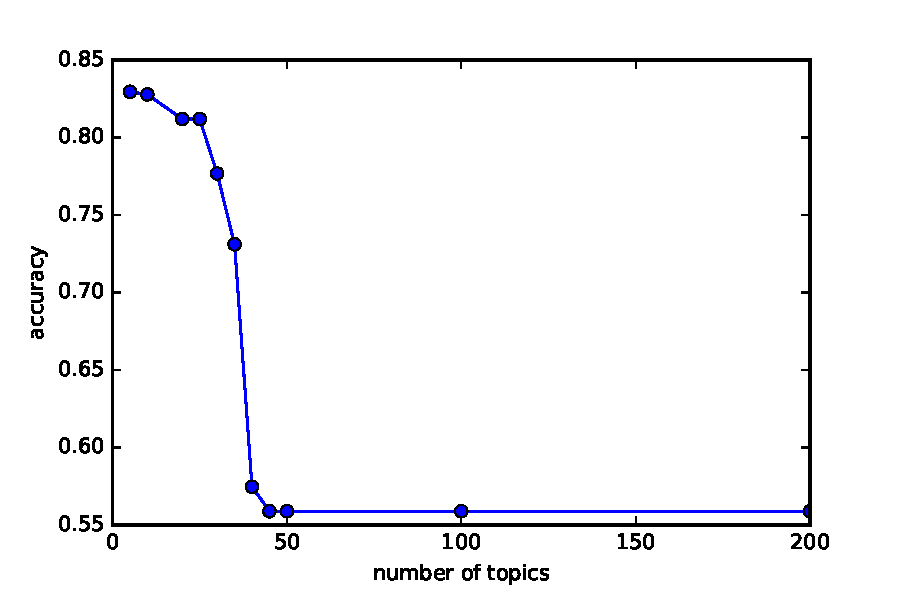
\includegraphics[width=0.7\textwidth]{plot_degradation_topic}
	\caption{A performance degradation issue observed when running BayesPA on small data with large number of topics}
\end{figure*}
\fi

\begin{itemize}
	\item {\bf Multiple Scans}: In this strategy, we simply scan the dataset for multiple passes. As shown in Figure~\ref{fg:solve_degradation}, this method works well --- with five passes, BayesPA can learn the topic model with more than 100 topics well and lead to improved accuracy when $K$ is in the range of $[50, 100 ]$. However, one disadvantage of this strategy is that it takes more computational resources, linear to the number of scans.
	\item {\bf Ghost Samples}: In this strategy, we create ghost copies of the data, that is, for every data point $(\xv_d, y_d)$, we make $L-1$ exact clones. Then in our global update equation, each aggregation of sufficient statistics will be multiplied by an extra factor of $L$. This strategy works well too, as shown in Figure~\ref{fg:solve_degradation}, although slightly worse than the strategy of multiple scans. One advantage of this strategy is that it does not increase the computation burden.
\end{itemize}
%Both approaches turned out to be effective, as shown in Figure ~\ref{fg:solve_degradation}.

\begin{figure*}[t]
\centering
	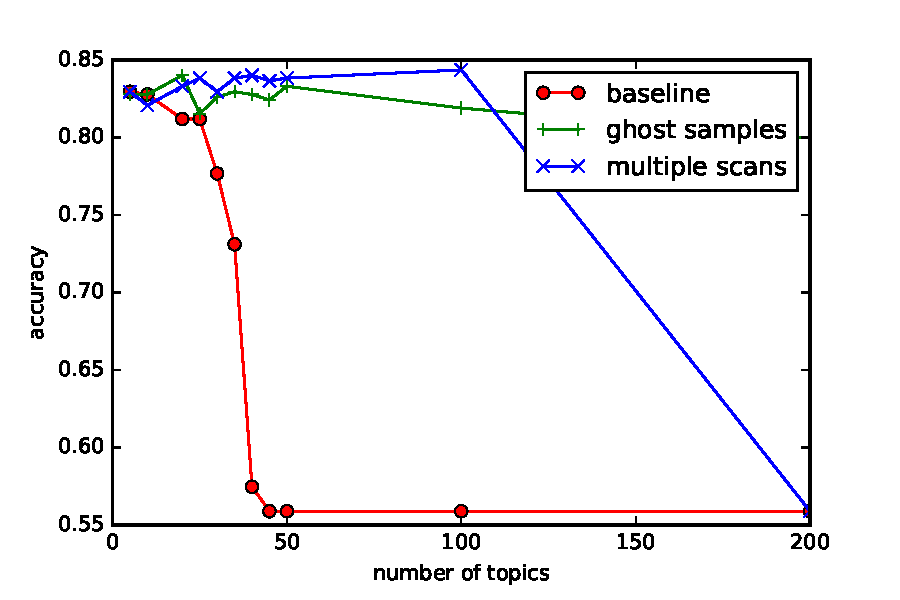
\includegraphics[width=0.7\textwidth]{plot_solve_degradation}
	\caption{Solving the performance degradation issue with a couple of practical approaches: \textbf{baseline}: the model without any modifications, where degradation issues emerge. \textbf{ghost copies}: create $L = 10$ copies for every mini-batch. \textbf{multiple scan}: run the model with total of five passes over the dataset.}
	\label{fg:solve_degradation}
\end{figure*}








\section{Conclusions and Future Work}
\label{sec:con}

We present online Bayesian Passive-Aggressive (BayesPA) learning as a new framework for max-margin Bayesian inference on streaming data. For fixed but large-scale data sets, online BayesPA effectively explores the statistical redundancy by repeatedly drawing samples and leads to faster convergence. We show that BayesPA subsumes the online PA, and more significantly generalizes naturally to incorporate latent variables and to perform nonparametric Bayesian inference, therefore providing great flexibility for explorative analysis. We provide provable regret bounds for the BayesPA models using either an averaging classifier or a Gibbs classifier. Based on the ideas of BayesPA, we develop efficient online learning algorithms for max-margin topic models as well as their nonparametric extensions which can automatically infer the unknown topic numbers. Empirical experiments on 20newsgroups and a large-scale Wikipedia multi-label data set demonstrate significant improvements on time efficiency, while maintaining comparable results.

\iffalse
Conceptually, we generalize the online Passive-Aggressive algorithms by \citep{crammer2006pa}, with new techniques developed to deal with latent variables. Empirically, we apply Bayesian PA learning to maximum entropy discriminant topic models and propose effective variational inference methods. Experiments on several real data sets demonstrate our approach yield results comparable to batch counterparts, while being significantly faster.
\fi


As for future work, we are interested in developing highly scalable, distributed \citep{broderick2013streaming} BayesPA learning paradigms, which will better meet the demand of processing massive real data available today. We are also interested in applying BayesPA to develop efficient algorithms for more sophisticated max-margin Bayesian models, such as the latent feature relational models~\citep{zhu2012maxlink}.


\section*{Acknowledgements}

This work is supported by National Key Foundation R\&D Projects (No. 2013CB329403), National Natural Science Foundation of China (Nos. 61322308, 61332007, 61305066), Tsinghua University Initiative Scientific Research Program (No. 20121088071), and a Microsoft Research Asia Research Fund (No. 20123000007).


\appendix

\section{}\label{app:regret-bound}
We provide the proof details to Theorem~\ref{tm:avg}.
\begin{proof}%\jun{can we defer this proof to appendix to make the main text clear?}
%\strin{I think the proof is important.}
%The proof is similar to that of Gibbs classifiers.
According to Lemma~\ref{lemma:avgBayesPA-Rep}, for BayesPA with averaging classifiers, we have the streaming update rule
\begin{equation*} %\label{eq:sol_bayespa}
q_{t+1}(\wv) = \frac{1}{\Gamma(\tau_t; \xv_t, y_t)} q_t(\wv) p(\xv_t | \wv)e^{\tau_t y_t \wv^\top \xv_t},
\end{equation*}
where $\Gamma(\tau_t; \xv_t, y_t)$ is the partition function and $\tau_t$ is the solution of the dual problem:
\begin{equation} \label{eq:bayespa_dual}
\max\limits_{0 \leq \tau \leq 2c}{\epsilon \tau - \log \Gamma(\tau; \xv_t, y_t)}.
\end{equation}
By definition, the partition function is
$\Gamma(\tau_t; \xv_t, y_t) = \int_{\wv}{q_t(\wv) p(\xv_t|\wv) e^{\tau_t y_t \wv_t \xv_t} d\wv}$. Construct the two parameter exponential family
\begin{equation*}
q_{t,\tau, u}(\wv) = q_t(\wv) \exp\Big(u \log p(\xv_t | \wv)+\tau y_t \wv^\top \xv_t-\log f(\tau, u)\Big),
\end{equation*}
where the log partition function $f(\tau, u)$ is
\begin{equation}
\log f(\tau, u) = \log \int_{\wv}{q_t(\wv) p(\xv_t | \wv)^u e^{\tau y_t \wv \xv_t} d\wv}. \nonumber
\end{equation}
\eat{which has the following properties
\begin{equation*}
\log f(0,0) = 0.
\end{equation*}
\begin{equation*}
\frac{\partial}{\partial u} f(\tau, u) = \ep_{q_{t,\tau, u}(\wv)}[\log p(\xv_t | \wv)].
\end{equation*}
\begin{equation*}
\frac{\partial}{\partial \tau} f(\tau, u) = \ep_{q_{t, \tau, u}(\wv)}[y_t \wv \xv_t].
\end{equation*}
\begin{equation*}
\frac{\partial^2}{\partial \tau \partial u} f(\tau, u) = \frac{\partial^2}{\partial u \partial \tau} f(\tau, u) = 0.
\end{equation*}}
Using Taylor's theorem again at the origin $(0,0)$, we have
\setlength\arraycolsep{1pt}\begin{eqnarray}
\log f(\tau, u) = && \ep_{q_t(\wv)} \left[\log p(\xv_t | \wv) \right] u +\E_{q_{t}(\wv)}\left[ y_t \wv^\top \xv_t \right] \tau  \nonumber \\
&& +\frac{1}{2} \Big(\var_{q_{\hat{\tau}, \hat{u}}}\left[y_t \wv \xv_t\right] \tau^2+\var_{q_{\hat{\tau}, \hat{u}}}\left[\log p(\xv_t | \wv)\right] u^2\Big), \nonumber
\end{eqnarray}
for some $0 < \hat{\tau} < \tau$ and $0 < \hat{u} < u$. Using our assumption on the fisher information and the fact that $\Gamma(\tau; \xv_t, y_t) = f(\tau, 1)$, we have the bound
\begin{equation} \label{eq:avg_key_bound}
\epsilon \tau - \log \Gamma(\tau; \xv_t, y_t) \geq -\ep_{q_t(\wv)} \left[\log p(\xv_t | \wv) \right]+\left( \epsilon-\E_{q_{t}(\wv)}\left[ y_t \wv^\top \xv_t \right] \right) \tau - \frac{1}{2} R \tau^2-\frac{1}{2} S.
\end{equation}
The optimal solution for the lower bound is $\tau^* = \min\{2c, (\epsilon-\E_{q_{t}(\wv)}[y_t \wv^\top \xv_t])/R\}$. Now, assume that the current round $q_t(\wv)$ suffers non-zero loss and consider the difference
\begin{equation}
\begin{array}{l}
\KL\left[p(\wv) || q_t(\wv)\right]-\KL\left[p(\wv) || q_{t+1}(\wv)\right]  \\
~~~~~~~ = \int_{\wv}{p(\wv) \tau_t\left( y_t \wv_t^\top \xv_t-\epsilon \right) d\wv}+\ep_{p(\wv)}[\log p(\xv_t | \wv)]+\Big(\epsilon \tau_t-\log \Gamma(\tau_t; \xv_t, y_t) \Big) \\
~~~~~~~ \geq -\regret_{c}^\text{ave}(p(\wv); \xv_t, y_t)+\Big(\epsilon \tau_t-\log \Gamma(\tau_t; \xv_t, y_t) \Big). \label{eq:kl_diff}
 \end{array}
\end{equation}
Notice that the second term in Eq.~(\ref{eq:kl_diff}) is exactly the optimization objective in the dual problem (\ref{eq:bayespa_dual}). Therefore, if $(\epsilon-\E_{q_{t}(\wv)}[y_t \wv^\top \xv_t]) \geq 2cR$, we have $\tau^* = 2c$ and use (\ref{eq:avg_key_bound}) to show
\begin{equation*}
\regret_c^\text{ave}(q_t(\wv); \xv_t, y_t) \leq \regret_{c}^\text{ave}(p(\wv); \xv_t, y_t)+ \KL[p || q_t]-\KL[p || q_{t+1}] +2 c^2 R + \frac{S}{2}.
\end{equation*}
If $(\epsilon-\E_{q_{t}(\wv)}[y_t \wv^\top \xv_t]) < 2cR$, we obtain

\eat{
bound on the squared loss
\begin{equation*}
\Big(\ell^\text{ave}_\epsilon(\xv_t)\Big)^2 \leq 2 \Big( \ell^*_\epsilon(\xv_t)+\frac{1}{c}(\KL[p || q_t]-\KL[p || q_{t+1}]) \Big) c R;
\end{equation*}
To unify the above two bounds, we can further simplify using the geometric inequality,
}

\begin{equation*}
\begin{array}{rl}
\ell^\text{ave}_\epsilon(q_t(\wv);\xv_t, y_t) \leq ~& 2 \sqrt{ c R \cdot \frac{1}{2c} \Big( \regret_c^\text{ave}(p(\wv); \xv_t, y_t)+\KL[p(\wv) || q_t(\wv)]-\KL[p(\wv) || q_{t+1}(\wv)]+S/2\Big)} \\\\
\leq ~&  c R +\frac{1}{2c} \Big( \regret_c^\text{ave}(p(\wv); \xv_t, y_t)+\KL[p(\wv) || q_t(\wv)]-\KL[p(\wv) || q_{t+1}(\wv)]+S/2\Big).
\end{array}
\end{equation*}
where we have used the geometric inequality. Summing over all $t = 0, 1, 2, ..., T-1$ gives (\ref{eq:avgnlpa_bound}) and further relax it by neglecting $\KL[p(\wv) || q_T(\wv)]$, we then derive Eq. (\ref{eq:avgnlpa_bound}).

\eat{
 Furthermore, by elementary calculus, one can show
\begin{equation*}
\log \cosh ( \tau \max_{\wv} |\wv^\top \xv_t| ) \leq (\tau \max_{\wv} |\wv^\top \xv_t|)^2.
\end{equation*}
We can use the above inequalities to bound (\ref{eq:bayespa_dual}), so the optimal $\tau_t$ also satisfy
\begin{equation} \label{eq:obj_bound}
\epsilon \tau_t - \log Z(\tau_t) \geq \max_{0 \leq \tau \leq c}{\tau (\epsilon-y_t \mathbb{E}_{q_{t}}[\wv^\top \xv_t])-(\tau |\max_{\wv} \wv^\top \xv_t|)^2}.
\end{equation}
where the maximization could be solved analytically leading to $\tau^* = \min(c, \frac{\epsilon-y_t \mathbb{E}_{q_{t}}[\wv^\top \xv_t]}{4 ( \max_{\wv} \wv^\top \xv_t)^2})$.
Combining (\ref{eq:obj_bound}) and (\ref{eq:kl_diff}), we can relate the losses at round $t$, denoted as $\ell_{\epsilon}(\xv_t)$ and $\ell^*_\epsilon(\xv_{t})$ as follows
\begin{equation}
\ell_{\epsilon}(\xv_t)^2 \leq 8 R^2 \Big( c \ell^*_{\epsilon}(\xv_{t})+(\KL[p || q_{t}]-\KL[p || q_{t+1}]) \Big).
\end{equation}
Summing over all $t \in [T]$, we have
\begin{equation}
\sum\limits_{t=1}^{T}{\ell_{\epsilon}(\xv_t)^2} \leq 8 R^2 \Big( c \sum\limits_{t=1}^{T}{\ell^*_{\epsilon}(\xv_{t})}+(\KL[p || q_{0}]) \Big).
\end{equation}
}
\end{proof}



\section{}\label{app:upperbound}
We show the objective in (\ref{eq:onlinepa_augmented}) is an upper bound of that in (\ref{eq:bayespa_latent}), that is,
%\begin{lemma}
%The following inequality holds true:
\begin{equation} \label{eq:varbound}
\mathcal{L}\Big( q( \wv, \Phiv, \Zv_t, \lambdav_t) \Big) -\mathbb{E}_q\Big[ \log(\psi(\Yv_t, \lambdav_t | \Zv_t, \wv)) \Big] \geq \mathcal{L}\Big( q( \wv, \Phiv, \Zv_t) \Big) + 2 c \sum\limits_{d \in B_t}{\mathbb{E}_q\Big[ (\xi_d)_+ \Big]},
\end{equation}
where $\mathcal{L}(q) = \KL[q || q_t(\wv, \Phiv) q_0(\Zv_t)]$.
%\end{lemma}

\begin{proof}
We first have
\begin{equation*}
\mathcal{L}\Big( q(\wv, \Phiv, \Zv_t, \lambdav_t) \Big) = \mathbb{E}_q\left[ \log \frac{q(\lambdav_t ~|~ \wv, \Phiv, \Zv_t) q(\wv, \Phiv, \Zv_t)}{q_t(\wv, \Phiv, \Zv_t)} \right],
\end{equation*}
and
\begin{equation*}
\mathcal{L}\Big( q(\wv, \Phiv, \Zv_t) \Big) = \mathbb{E}_q\left[ \log \frac{q(\wv, \Phiv, \Zv_t)}{q_t(\wv, \Phiv, \Zv_t)} \right].
\end{equation*}
Comparing these two equations and canceling out common factors, we know that in order for (\ref{eq:varbound}) to make sense, it suffices to prove
\begin{equation}\label{eq:boundlemma_entropy}
\mathbb{H}[q']-\mathbb{E}_{q'}[\log(\psi(\Yv_t, \lambdav_t | \Zv_t, \wv)] \geq 2 c \sum\limits_{d \in B_t}{\mathbb{E}_{q'}[(\xi_d)_+]}
\end{equation}
is uniformly true for any given $(\wv, \Phiv, \Zv_t)$, where $\mathbb{H}(\cdot)$ is the entropy operator and $q' = q(\lambdav_t ~|~ \wv, \Phiv, \Zv_t)$. The inequality (\ref{eq:boundlemma_entropy}) can be reformulated as
\begin{equation} \label{eq:boundlemma}
\mathbb{E}_{q'}\left[ \log \frac{q'}{\psi(\Yv_t, \lambdav_t | \Zv_t, \wv)} \right] \geq 2c \sum\limits_{d \in B_t}{\mathbb{E}_{q'}[(\xi_d)_+]}
\end{equation}
Exploiting the convexity of the function $\log(\cdot)$, i.e.
\small
\begin{equation*}
-\mathbb{E}_{q'}\left[ \log \frac{\psi(\Yv_t, \lambdav_t | \Zv_t, \wv)}{q'} \right]  \geq -\log \int_{\lambdav_t}{\psi(\Yv_t, \lambdav_t | \Zv_t, \wv) ~d\lambdav_t},
\end{equation*}
\normalsize
and utilizing the equality (\ref{eq:scalemix}), we then have (\ref{eq:boundlemma}) and therefore prove (\ref{eq:varbound}).
\end{proof}

\vskip 0.2in

\bibliography{BayesPA}

\end{document} 